\documentclass[a4paper,12pt]{article}
%\usepackage[cp1251]{inputenc}
\usepackage{graphicx,color}
\usepackage{amssymb}
\usepackage{amsmath}
\usepackage[T2A]{fontenc}
\usepackage[utf8]{inputenc}
\usepackage[english,russian]{babel}
\usepackage{geometry}
\usepackage{lastpage}
\usepackage[figure]{totalcount}
\usepackage{subfig}
\usepackage[numbib]{tocbibind}
\usepackage{cite}
\usepackage{titlesec}
\usepackage{enumitem}
\usepackage{totcount}
\usepackage{tikz}
% This is necessary to split formula inside brakets
\usepackage{breqn}
% \usepackage{pgfplots}
% \usepgfplotslibrary{external}
% \pgfplotsset{compat=1.10}
% \tikzexternalize

\DeclareUnicodeCharacter{00A0}{}

\bibliographystyle{ugost2008}

% \newcommand{\sectionbreak}{\clearpage}

\renewcommand{\floatpagefraction}{0.6}

\linespread{1.25}           %-интервал между строками

\righthyphenmin=2 \textwidth = 17cm \oddsidemargin = -.54cm \topmargin = -1.54cm \textheight = 25 cm

\begin{document}
\newtotcounter{citnum}
\def\oldbibitem{} \let\oldbibitem=\bibitem
\def\bibitem{\stepcounter{citnum}\oldbibitem}
\sloppy                             %-выравнивание по правому краю
\sloppy                             %-выравнивание по правому краю
\titlepage
\begin{center}
ГОСУДАРСТВЕННАЯ КОРПОРАЦИЯ ПО АТОМНОЙ ЭНЕРГИИ <<РОСАТОМ>>
\end{center}

\vspace{.15cm}

\hrule height 1.5pt

\vspace{.2cm}

\hspace{6cm} \scriptsize{ФЕДЕРАЛЬНОЕ ГОСУДАРСТВЕННОЕ УНИТАРНОЕ ПРЕДПРИЯТИЕ}

\hspace{-.65cm}
\includegraphics[width=2.5cm]{images/Logotip} \hspace{0.2cm}\vspace{-0.5cm}\Huge{\bfseries ВНИИА}
\vspace{-1.7cm}\small
\begin{center}
\hspace{6.5cm}{\bfseries ВСЕРОССИЙСКИЙ}

\hspace{6.5cm}{\bfseries НАУЧНО-ИССЛЕДОВАТЕЛЬСКИЙ ИНСТИТУТ}

\hspace{6.5cm}{\bfseries АВТОМАТИКИ }

\hspace{6.5cm}{\bfseries им. Н.Л. ДУХОВА}
\end{center}

\hrule height 1.5pt

\normalsize

\begin{flushright}

%\vspace{.1cm}

%\begin{list}{}{\leftmargin=10,1cm}
%\vspace{-0.15cm}{\bfseries Для служебного пользования}
%\vspace{-0.15cm}{\bfseries Экз. № }\underline{~~~~~~~~~~~~~~~~~~~~~~~}
%\end{list}eq
\vspace{.2cm}


\end{flushright}

%\vspace{-0.1cm}
\begin{flushleft}
{\bfseries УДК\underline{\hspace{1cm}539.171, 539.144\hspace{1. cm}}}\\
%{\bfseries Номер государственной}\\
%{\bfseries регистрации\underline{\hspace{2.3cm}}}\\
{\bfseries Инв.\textnumero\underline{\hspace{1.5cm}70/       \hspace{1.5 cm}}}
\end{flushleft}
\vspace{-1.8cm} {\begin{list}{}{\leftmargin=10,4cm}
\vspace{-0.15cm}\item{\bf<<УТВЕРЖДАЮ>>}
\vspace{-0.15cm}\item{\bfseries Научный руководитель}
\vspace{-0.15cm}\item{\bfseries ФГУП ВНИИА, д.ф.-м.н.}
\vspace{-0.15cm}\item\underline{~~~~~~~~~~~~~~~~~~~~~~~}~{\bfseries А.В. Андрияш}
\vspace{-0.15cm}
\item{\bf<<\underline{~~~~~}>>}\underline{~~~~~~~~~~~~~~~~~~~~~~~~~~}~{\bf2019 г.}
\end{list}}

%\vspace{0.1cm}

\large

\begin{center}
%\vspace{-0.5cm}{\bfseries ОТЧЕТ}

\vspace{.2cm}


{\bfseries Научно-технический отчёт\\
 Создание собственной геометрической ТРТ оболочки для моделирования радиационного транспорта, позволяющей работать без Geant4-интерфейса и полностью контролировать вычисления, освободившись от ограничений, накладываемых интерфейсом Geant4.
}

%\vspace{0.5cm} \small \emph{Шифр темы <<Сочетание>>}
\vspace{0.2cm} \emph{Шифр темы <<Сочетание>>}
\end{center}

\vspace{-.2cm}

\normalsize

\vspace{0.1 cm}
\begin{flushright}
Начальник подразделения 70 \\
\underline{~~~~~~~~~~~~~~~~~~~~~~~}~{ С.Е. Куратов}\\
<<\underline{~~~~~}>>\underline{~~~~~~~~~~~~~~~~~~~~~~~~~~}~2019 г. \\
\vspace{0.2 cm}
\emph{Ответственные исполнители}:\\
\vspace{0.1 cm}
Главный научный сотрудник, д.ф.-м.н.\\
\underline{~~~~~~~~~~~~~~~~~~~~~~~}~{ М.В. Косов}\\
<<\underline{~~~~~}>>\underline{~~~~~~~~~~~~~~~~~~~~~~~~~~}~2019 г.\\
\vspace{0.1 cm}
Научный сотрудник\\
\underline{~~~~~~~~~~~~~~~~~~~~~~~}~{ Д.И. Савин}\\
<<\underline{~~~~~}>>\underline{~~~~~~~~~~~~~~~~~~~~~~~~~~}~2019 г.\\
\vspace{0.1 cm}
Младший научный сотрудник\\
\underline{~~~~~~~~~~~~~~~~~~~~~~~}~{ А.А. Галюзов}\\
<<\underline{~~~~~}>>\underline{~~~~~~~~~~~~~~~~~~~~~~~~~~}~2019 г.\\
\vspace{.4 cm}
\end{flushright}
\begin{center}
Москва 2019
\end{center}

\newpage
\renewcommand\abstractname{Реферат}
\abstract{

Объём отчета
\pageref{LastPage} страниц c
\totalfigures\ рисунками и списком литературы из
\total{citnum}\ ссылок.

  Ключевые слова: Geant4, TPT, метод Монте-Карло, транспорт ионов, ионный каскад.

  	Программный комплекс ТРТ, разработанный во ВНИИА, предназначен для моделирования транспорта ионов, элементарных частиц и нейтронного излучения в различных материалах, а также для моделирования протекающих при этом ядерных реакций.
  	При этом ТРТ, в отличие от хорошо известной программы MCNP, осуществляет эксклюзивное моделирование ядерных реакций, т. е. сохраняет энергию и импульс в каждом взаимодействии.
  
  	Используя для моделирования свои собственные физические библиотеки и базы данных, ТРТ в качестве основы и структуры организации кода использует классы и интерфейсы программного комплекса Geant4.
  	В Geant4 используется сложная многоуровневая иерархия наследования классов, что приводит к большей универсальности программного кода.
  	В свою очередь использование многоуровневого наследования и сложной иерархии классов приводит к уменьшению производительности программного кода.
  	Также в Geant4 существует очень детальная  система описания геометрических объёмов, которая усложняет и опять же замедляет моделирование, а в некоторых случаях приводит к неопределённому поведению, например, при движении заряженных частиц во внешнем магнитном поле вблизи границы раздела 2 сред.
  
  	Задачей данного отчёта является создание версии ТРТ3 программного комплекса ТРТ (последней версией которого на данный момент является версия TPT2), основанной на разработанном параллельном ТРТ-навигаторе частиц, использующем максимально возможные распараллеливание кода по OpenMP потокам и его векторизацию.
  	Это позволит моделировать все частицы параллельно и не зависимо друг от друга.
  	Само по себе ограничение иерархии наследования классов даже без учёта распараллеливания кода по OpenMP потокам и векторизации приведёт к его более высокому быстродействию, чем Geant4.
  	Использование упрощённой воксельной геометрии позволит упростить описание моделируемых объёмов и дополнительно повысить производительность моделирования.
  
  	Отдельной задачей является сделать так, чтобы разработанный программный код работал и на CPU, и на GPU.
  	Это большая и сложная работа, т. к. архитектуры CPU и GPU различны, и не все операции, которые стандартно работают на CPU, работают и на GPU.
  	Это приводит к необходимости изменять архитектуру программного кода и используемые алгоритмы так, чтобы они работали на GPU.
  
}

\newpage

\tableofcontents

\begin{large}

\clearpage
\section{Введение}
\label{Intr}
% magic phrase for the quarterly report
  	В отчёте использованы результаты работ, выполненных в ФГУП ВНИИА в четвёртом квартале 2019 года в рамках темы "СОЧЕТАНИЕ": "Создание собственной геометрической ТРТ оболочки для моделирования радиационного транспорта, позволяющей работать без Geant4-интерфейса и полностью контролировать вычисления, освободившись от ограничений, накладываемых интерфейсом Geant4.".

    Программный комплекс ТРТ (Toolkit for Particle Transport, Теоретико-Числовой Радиационный Транспорт) создан во ВНИИА для моделирования транспорта элементарных частиц и ионов с сохранением энергии, импульса и квантовых чисел в каждом ядерном взаимодействии.
    Такой подход к моделированию ядерных реакций называется эксклюзивным в отличие от инклюзивного подхода, не учитывающего законы сохранения и моделирующего лишь средние потоки радиации подобно тому, как моделируется оптический спектр фотонов, приходящих к нам от далёких звёзд.
    Инклюзивный подход к моделированию использует, например, программа MCNP.
    
    Используя свои библиотеки физических процессов и базы данных сечений ядерных реакций, ТРТ основывается на интерфейсе программного комплекса Geant4 \cite{Geant4.1}.
    Это означает, что вся сложная иерархия наследования классов и интерфейсов, а также непростые взаимные связи между объектами, заложенные разработчиками Geant4, присутствуют и в ТРТ.
    
    Допустим, есть базовый класс -- интерфейс с виртуальными функциями, и есть классы-наследники, которые эти виртуальные функции переопределяют.
    А также имеется указатель на базовый класс, которому в разные моменты времени работы программы присваиваются адреса объектов различных производных классов, т. е. указатели на них.
    Как известно, при динамическом связывании в С++, то, какая функция будет вызываться, определяется по типу объекта, адрес которого хранит указатель, который её вызывает.
    Это реализуется с помощью так называемых виртуальных таблиц, имеющихся для каждого класса, у которого есть виртуальный метод.
    То, что связывание происходит во время работы программы, мешает компилятору встроить (inline) и  как-либо оптимизировать код вызова виртуальных функций.
    Это приводит к определённым временным задержкам при вызовах виртуальных функций в С++, особенно если имеется многоуровневая иерархия наследования.
    К тому же, различные связи между классами, которые заложили в Geant4 его разработчики, сильно затрудняют поиск ошибок, когда сложность моделирования возрастает.
    Но, главное, это уменьшает эффективность распараллеливания кода, сокращая его производительность.
    
    В Geant4 существует сложная система моделирования различных физических объёмов.
    Это делает его универсальным, позволяя моделировать прохождение излучений через физические объёмы практически любой сложности.
    Но это также серьёзно замедляет моделирование и создаёт ряд проблем при моделировании движения частиц вдоль границ раздела нескольких различных физических объёмов.
    Например, когда заряженная частица движется вдоль границы раздела 2 различных сред в магнитном поле, она движется поступательно и вращается по ларморовскому радиусу.
    Т. к. шаг моделирования конечен, а граница раздела рассматривается не как бесконечно тонкая математическая поверхность, а как слой, имеющий конечную толщину, в некоторых случаях возникает неопределённое поведение программы.
    И адекватного моделирования этого явления в Geant4, позволяющего избежать возникновения неопределённого поведения в таких случаях, до сих пор не создано.
    
    Поэтому стоит задача создания на основе разработанного параллельного навигатора частиц ТРТ3 версии программного комплекса ТРТ, позволяющей работать без Geant4-интерфейса и полностью контролировать вычисления, освободившись от ограничений, накладываемых интерфейсом Geant4.
    Также для повышения производительности и упрощения моделирования предлагается отказаться от сложного описания физических объёмов, используемого в Geant4, и моделировать физические объёмы, заполненные различными материалами, с помощью вокселей (ячеек декартовой сетки).
    Воксели могут быть адаптивными, их можно разделять на части секущими плоскостями, так что с помощью воксельной геометрии вполне возможно создать собственную геометрическую ТРТ оболочку для моделирования радиационного транспорта.
    
    Также планируется сделать так, чтобы разрабатываемый программный код работал и на CPU, и на GPU.
    Т. е. чтобы с помощью простой замены флагов компиляции можно было компилировать исполняемый файл для запуска и на центральном процессоре, и на графическом ускорителе.
    Для распараллеливания кода для запуска на GPU используется компилятор PGI \cite{PGI} и стандарт препроцессорных директив OpenAcc \cite{OpenAcc}.
    Это сложная задача, т. к. архитетуры CPU и GPU различны, и не все стандартные операции, работающие на CPU, будут работать и на GPU.
    Например, на GPU нельзя использовать стандартные C++ контейнеры $array$, $vector$, $tuple$ и $map$, можно использовать только массивы языка С.
    Также нельзя использовать $extern$ и $static$ переменные, а также переменные типа $long$ $double$.
    В параллельных участках кода, исполняемых на GPU, невозможно выделять память, например создавать С массивы.
    Серьёзным ограничением стало то, что на GPU не поддерживаются виртуальные функции и наследование. 		Эти и другие ограничения привели к тому, что пришлось изменить архитектуру разрабатываемого программного кода и изменить многие используемые методы так, чтобы они работали на GPU.
    
    Первой задачей, на которой применяется разрабатываемый программный код, является моделирование ионного каскада в мишени из дейтерида титана, облучаемой интенсивным потоком дейтронов.
    Для её реализации было необходимо к разработанному программному интерфейсу, основывающемуся на параллельном навигаторе частиц ТРТ3, добавить реализации физических процессов многократного рассеяния, упругого ион-ионного рассеяния и неупругого D-D рассеяния и провести валидацию (проверку и сравнение с базами данных) полученных угловых распределений на используемом параллельном и векторизованном программном коде.
    После чего можно было переходить к самому моделированию. 
   
   Создание собственной хорошо протестированной и качественной программы радиационного транспорта -- это очень большая работа, и малыми силами можно только отработать технологии и обеспечить необходимыми базами данных только ограниченное количество веществ для конкретного применения.
   Однако постепенно, от задачи к задаче, базы данных для различных материалов будут пополняться.
   
   
\clearpage{}
\section{Валидация углового распределения многократного рассеяния ионов в дейтерида титана.}
\label{ValMS}

\subsection{Аппроксимация функции плотности вероятности углового распределения многократного рассеяния.}
\label{subValMS1}

	В предыдущем отчёте \cite{70/778-T} была получена аппроксимация функции плотности вероятности углового распределения многократного рассеяния в зависимости от длины пробега в материале мишени $x$ для дейтронов с энергией 10 МэВ, падающих на мишень из дейтерида титана перпендикулярно торцу мишени.
 
	Аппроксимация функции плотности вероятности углового распределения многократного рассеяния дейтронов на ионах кристаллической решётки $TiD_2$ проводилась на основе следующей функции, описывающей центральное распределение Гаусса с добавленными гауссовыми членами ``носа'' и ``хвоста'' \cite{70/778-T}:
\begin{equation}
\label{MSApproximationFunction}
\begin{aligned} 
  f(\theta,\,x)=\sum_{i=1}^{3} \frac{2W_i(x)}{D_i(x)}e^{-\frac{\theta^2}{D_i(x)}}.
\end{aligned}
\end{equation}
  	Первый член суммы ($i=1$) описывает ``нос'' распределения, который соответствует вкладу ещё не гауссизировавшегося углового распределения многократного рассеяния, когда длина пробега частиц в мишени ещё очень мала.
  	Второй ($i=2$) -- основной гауссиан, только который везде и принято использовать \cite{PDG}.
  	Третий член ($i=3$) --  ``хвост'' распределения, который имеет смысл рассеяния на большие углы, и который в \cite{PDG}, как это там написано, не учитывается, т. к. его вклад в общее распределение мал, и им пренебрегают.
  
  	Результаты аппроксимации интегральных величин $W_i(x)$, имеющих смысл вкладов гауссоид в общее распределение, представляются функциями:
  
\begin{equation}
\label{MSApproximationW1}
\begin{aligned} 
  W_1(x)= \frac{33390\cdot (1+\left(\frac{x}{17.1}\right)^{0.88})}{x^{0.12} \cdot \left(1+\left(\frac{x}{0.636}\right)^{1.16}\right) \cdot \left(1+\left(\frac{x}{6.128}\right)^{2.05}\right)},
\end{aligned}
\end{equation}

\begin{equation}
\label{MSApproximationW2}
\begin{aligned} 
  W_2(x)= \frac{22979\cdot \left(1+\frac{0.0717}{x}\right)\cdot \left(1+\left(\frac{x}{9.628}\right)^{0.032}\right)}{1+\frac{0.27}{x}}
\end{aligned}
\end{equation}

и

\begin{equation}
\label{MSApproximationW3}
\begin{aligned} 
  W_3(x)= \frac{21859}{x^{0.09}\cdot\left(1+\left(\frac{0.8884}{x}\right)^{1.08}\right)},
\end{aligned}
\end{equation}

	где $x$ -- длина пробега дейтронов в материале мишени в микронах.
	Зависимости $W_1(x)$-$W_3(x)$ изображены на Рис. ~\ref{fig:Par1theta}. Пунктирной горизонтальной линией показана их сумма -- нормировка, которая должна быть константой.

\begin{figure}[ht]
  {
     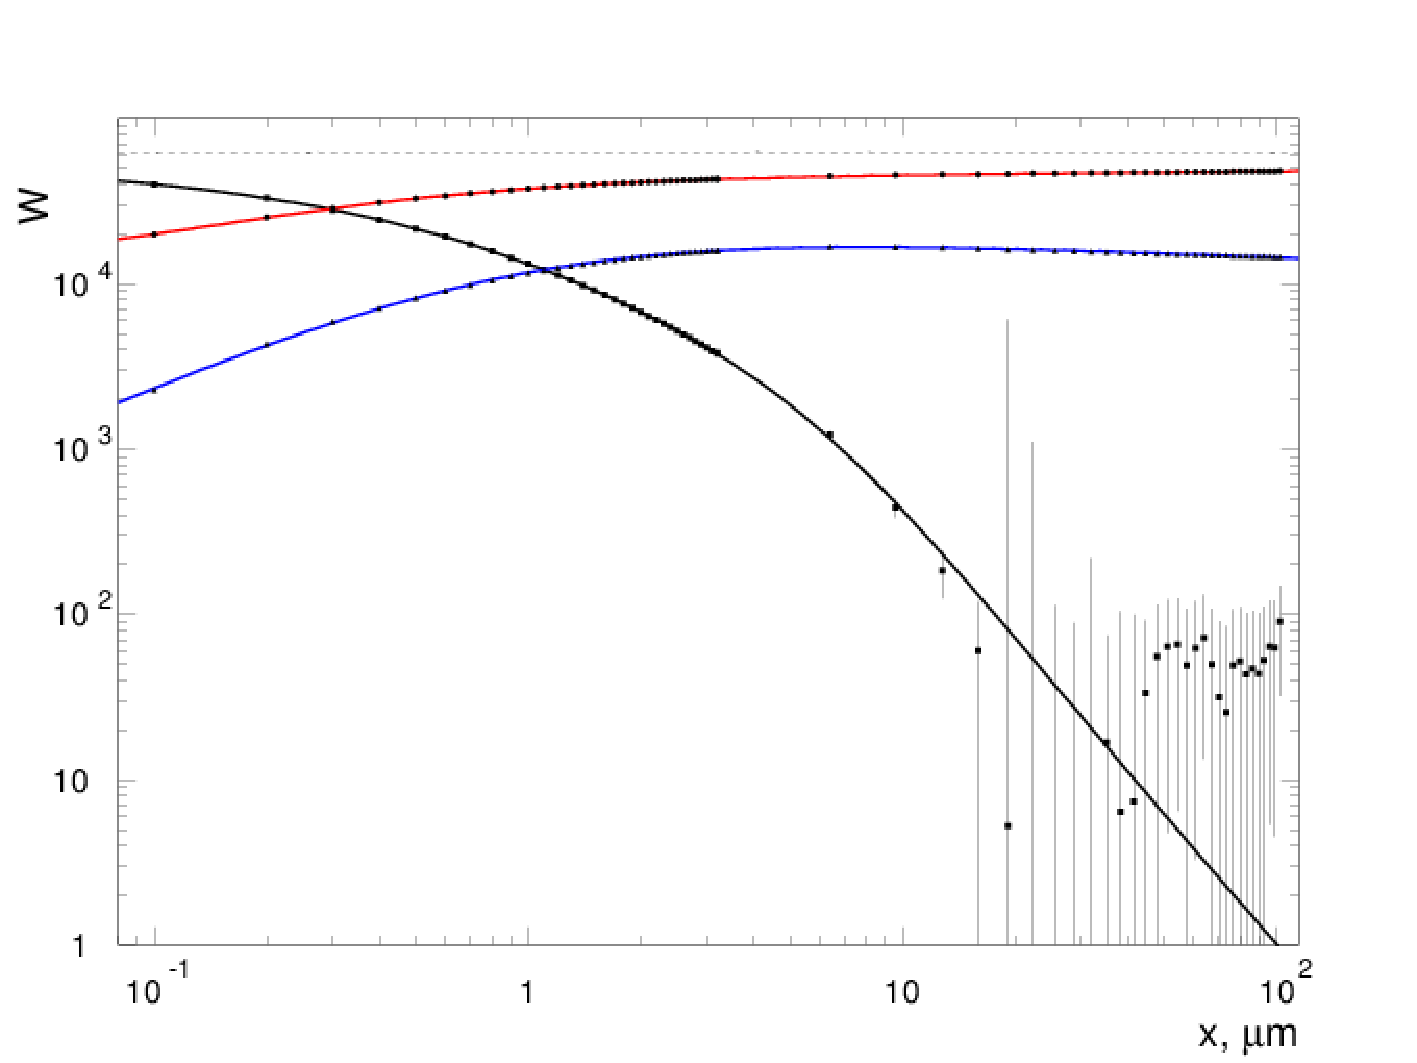
\includegraphics[width=0.99\linewidth]{images/pars135}
  }
  \caption{Изменение интегралов трёх гауссовых кривых с увеличением пробега дейтронов $x$ в материале мишени.}
  \label{fig:Par1theta}
\end{figure}

	На Рис. ~\ref{fig:DispTheta} показан рост удвоенной дисперсии гауссианов при увеличении пробега дейтрона в материале мишени:

\begin{equation}
\label{MSApproximationD1}
\begin{aligned} 
  D_1(x)=\frac{0.59\cdot 10^{-5}\cdot x}{1+\frac{0.029}{x}}, 
\end{aligned}
\end{equation}

\begin{equation}
\label{MSApproximationD2}
\begin{aligned} 
  D_2(x)=D_1(x)+0.854\cdot 10^{-6}\cdot\left( 1+\left(\frac{x}{0.25} \right)^{1.108}\right)
\end{aligned}
\end{equation}

и

\begin{equation}
\label{MSApproximationD3}
\begin{aligned} 
  D_3(x)=D_2(x)+0.8\cdot 10^{-5}\left( 1+\left(\frac{x}{1.28} \right)^{0.77}\right)\cdot\left( 1+ \left(\frac{x}{132.37} \right)^{4.64}\right).
\end{aligned}
\end{equation}

\begin{figure}[ht]
  {
     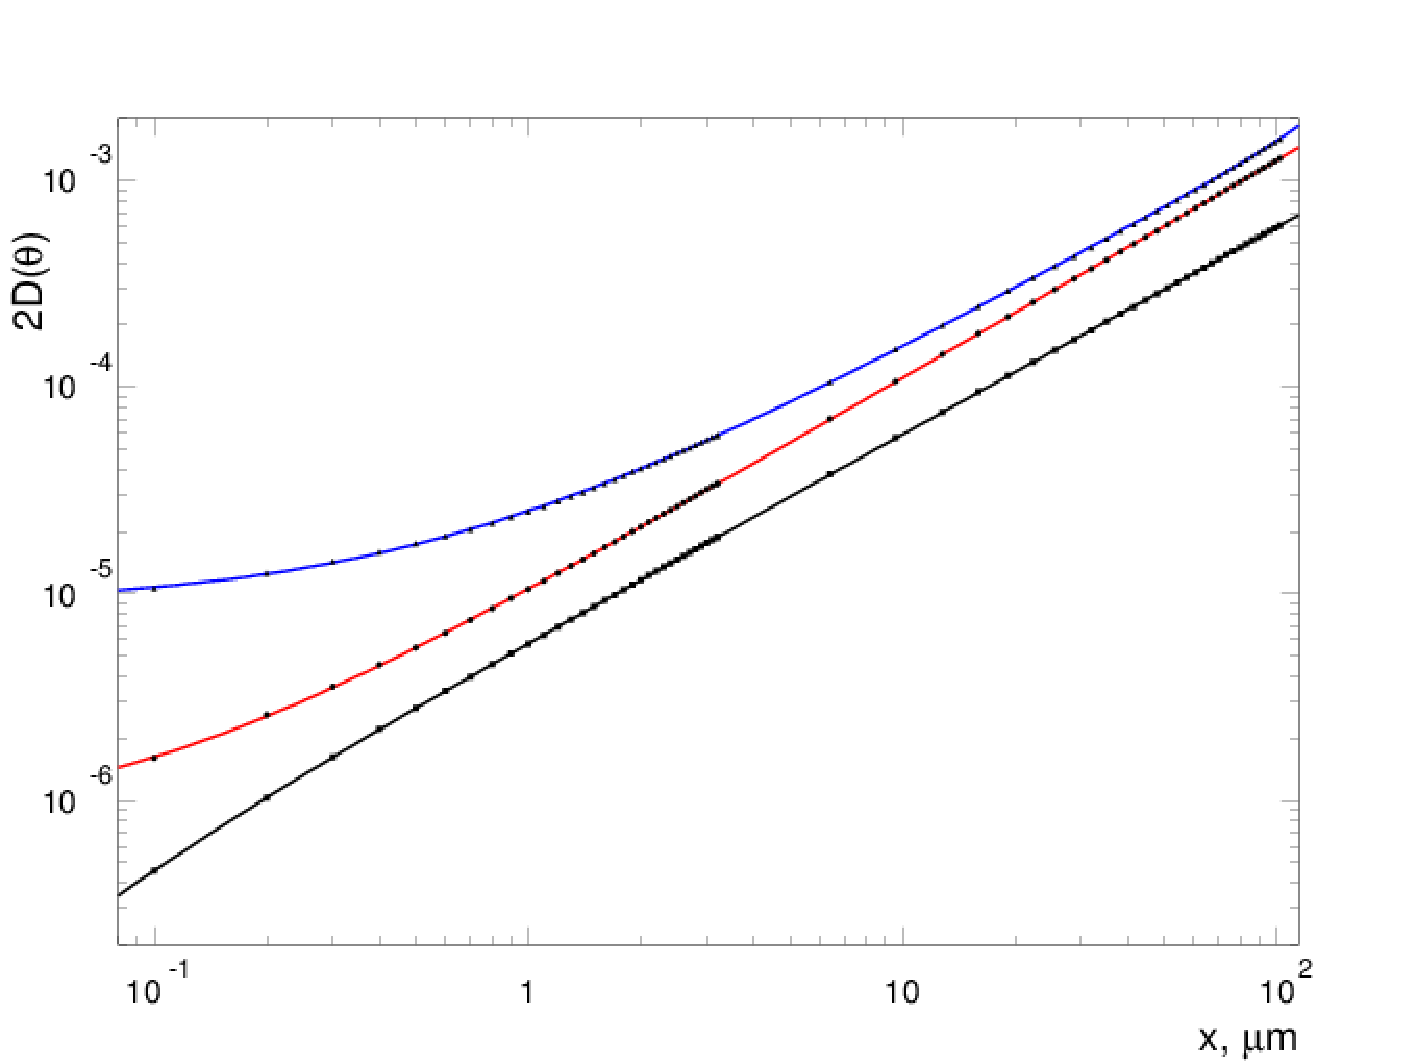
\includegraphics[width=0.99\linewidth]{images/pars246}
  }
  \caption{Изменение дисперсий трёх гауссовых кривых с увеличением толщины слоя.}
  \label{fig:DispTheta}
\end{figure}

	Заметим, что данный результат был получен для случая, когда большие переданные импульсы в Резерфордовском рассеянии обрезаны и перенесены в дискретное моделирование.
	Осуществление передачи больших импульсов реализуется в дискретном процессе упругого рассеяния, в котором, в свою очередь, нет передачи малых импульсов, которая реализуется с помощью полученной аппроксимации и непрерывного процесса многократного рассеяния, включённого в моделирование.
  	Если пытаться учесть полное Резерфордовское рассеяние, вклад ``хвоста'' будет значительно больше, и он будет падать значительно медленнее, чем гауссово распределение.
  	По этой причине в реальных экспериментах обнаруживаются широкие ``крылья'', которые при использовании данной аппроксимации будут определяться дискретным рассеянием, учитывающим интерференцию электромагнитной и сильной амплитуд рассеяния.
  
  	Также следует отметить, что данный результат был получен для многократного рассеяния в мишени из дейтерида титана дейтронов с начальной кинетической энергией $T_{LS}$=10 МэВ.
  	Для использования полученной функции плотности вероятности углового распределения многократного рассеяния при других энергиях налетающих дейтронов, а также для углового распределения многократного рассеяния ионов титана в мишени из дейтерида титана, необходимо предложить некий метод пересчёта, скейлинг, позволяющий экстраполировать её область применимости с $Z=1$, $A=2$ и $T_{LS}$=10 МэВ на произвольные $T_{LS}$ и ионы титана.
  
\subsection{Пересчёт полученной аппроксимации углового распределения многократного рассеяния для произвольной кинетической энергии налетающих дейтронов и ионов титана.}
\label{subValMS2}

	Как известно, обычно для описания углового распределения многократного рассеяния используют одно распределение Гаусса, которое соответствует основному гауссиану в  (\ref{MSApproximationFunction}), т. е. вклады распределений ``носа'' и ``хвоста'' в угловое распределение многократного рассеяния обычно не учитываются.
	С помощью аппроксимации экспериментальных данных получено выражение для полуширины на полувысоте такого Гауссова распределения для широкого диапазона налетающих частиц и материалов \cite{PDG}:
\begin{equation}
  \label{Theta0}
  \theta_0(x)=\frac{13.6 \cdot z \cdot \sqrt{\frac{x\cdot \rho}{X_0}}}{\beta_{LS}\cdot p_{LS}}\cdot\left[ 1+0.038\cdot\ln\left(\frac{x\cdot \rho}{X_0}\right)\right],
\end{equation}	

	При учёте $\beta_{LS}=\frac{p_{LS}}{E_{LS}}$ формула (\ref{Theta0}) принимает вид:
\begin{equation}
  \label{CheckTheta0Coefficient}
  \theta_0(x)=13.6 \cdot z \cdot \sqrt{\frac{x\cdot \rho}{X_0}} \cdot \frac{E_{LS}}{p^2_{LS}} \cdot\left[ 1+0.038\cdot\ln\left(\frac{x\cdot \rho}{X_0}\right)\right],
\end{equation}
	где $\frac{x}{X_0}$ -- толщина рассеивающей среды в единицах радиационной длины $X_0$, измеряемой в г/см$^2$.
	Для пересчёта $X_0$ в единицы длины используется плотность $\rho_{TiD_2}=3.91$ г/см$^3$.
	А $z$, $E_{LS}$ и $p_{LS}$ -- заряд, энергия и импульс налетающей частицы в лабораторной системе, измеряемые в МэВ.
	Для налетающего дейтрона с массой покоя $m_D=1875.6$ МэВ и кинетической энергией $T_{LS}=10$ МэВ его импульс $p_{LS}=193.94$ МэВ и полная энергия $E_{LS}=1885.6$ МэВ.
	Радиационная длина $TiD_2$ вычисляется из соотношения:
\begin{equation}
  \label{RadLength}
  \frac{A_{TiD_2}}{X_{0_{TiD_2}}}=\frac{2 A_{D}}{X_{0_{D}}}+\frac{A_{Ti}}{X_{0_{Ti}}},
\end{equation}
	где $A_i$ -- масса молекулы/элемента в атомных единицах массы (а.е.м.), а $X_{0_i}$ -- радиационная длина.
  	Так как $A_{TiD_2}=51.89$, $A_{D}=2.01$ и $A_{Ti}=47.87$, а также $X_{0_{D}}=125.98$ г/см$^2$ и $X_{0_{Ti}}=16.16$ г/см$^2$ \cite{PDG}, то $X_{0_{TiD_2}}=17.33$ г/см$^2$, что эквивалентно $\frac{X_{0_{TiD_2}}}{\rho_{TiD_2}}=4.43$ см.
  
  	Из формулы (\ref{CheckTheta0Coefficient}) можно получить, что дисперсия соответствующего углового распределения равняется

\begin{equation}
  \label{Theta0Dispersion}
  \begin{aligned}
   D(x)=2 \cdot \theta^2_0(x)=2 \cdot 13.6^2 \cdot z^2 \cdot \frac{x\cdot \rho}{X_0} \cdot \frac{E^2_{LS}}{p^4_{LS}} \cdot\left[ 1+0.038\cdot\ln\left(\frac{x\cdot \rho}{X_0}\right)\right]^2.
   \end{aligned}
\end{equation}

  
  	Можно заметить, что величина $0.038\cdot\ln\left(\frac{x\cdot \rho}{X_0}\right)$ мала по сравнению с 1 при $x$ вплоть до десятков мкм, поэтому при моделировании толстой мишени из дейтерида титана, в которой произошла гауссизация углового распределения многократного рассеяния (для этого требуется, чтобы каждая частица перерассеялась много раз), ей можно пренебречь.
  	При моделировании же тонкой мишени, где вклад этой величины был бы значителен, формулой  (\ref{CheckTheta0Coefficient}) пользоваться нельзя, т. к. гауссизации углового распределения многократного рассеяния в результате большого количества перерассеяний частиц ещё не произошло, и поэтому трудно говорить об угловом распределении многократного рассеяния при малых $x$.
  
  	Из выражения (\ref{Theta0Dispersion}) видно, что $D(x) \sim z^2 \cdot \frac{E^2_{LS}}{p^4_{LS}} \cdot x$.
  	Получающаяся зависимость $D(x)$ совпадает по форме с основным гауссианом (\ref{MSApproximationD2}), если в нём пренебречь малым добавочным слагаемым с коэффициентом порядка $10^{-6}$.
  	Т. к. при аппроксимации рассматриваются $x \geq 1$ мкм, выражение в знаменателе (\ref{MSApproximationW2}) стремится к 1.
  	В связи с этим в качестве скейлиногового коэффициента пересчёта для других $E_{LS}$ и $z$ было выбрано выражение $z^2 \cdot \frac{E^2_{LS}}{p^4_{LS}}$.
  
  	Таким образом, в первом приближении, пересчёт аппроксимации функции плотности вероятности углового распределения многократного рассеяния для налетающих частиц с другой $E_{LS}$ и другим $z$ проводился следующим образом.
  	Вклады каждого из гауссианов $W_1$-$W_3$ брались без изменений.
  	А для их дисперсий $D_1$-$D_3$ выполнялось следующее: каждая $D_i$ делилась на $\frac{E^2_{LS}}{p^4_{LS}}$ для налетающего дейтрона с энергией 10 МэВ (для дейтрона $z=1$), т. к. аппроксимация (\ref{MSApproximationFunction}) была получена для налетающих дейтронов с энергией 10 МэВ, и умножалась на $z^2 \cdot \frac{E^2_{LS}}{p^4_{LS}}$ для налетающей частицы с $E_{LS}$ и $z$, для которой необходимо было пересчитать аппроксимацию функции плотноости вероятности углового рапределения многократного рассеяния:
  	
\begin{equation}
  \label{DispersionScaling}
   \tilde D_i(x)[E_{LS}, z]=\frac{D_i(x) \cdot p^{4}_{LS}[D, 10 MeV]}{E^{2}_{LS}[D, 10 MeV]} \cdot z^2 \cdot \frac{E^{2}_{LS}}{p^{4}_{LS}}.
\end{equation}  

	Полученная таким образом аппроксимация функции плотности вероятности углового распределения многократного рассеяния, применимая и для ионов дейтерия, и для ионов титана, при произвольных энергиях, использовалась при моделировании ионного каскада в мишени из дейтерида титана для описания непрерывного процесса многократного рассеяния частиц в веществе мишени.

	При помощи описанного способа скейлинга были получены угловые распределения функции плотности вероятности углового распределения многократного рассеяния для движущихся в мишени из дейтерида титана ионов дейтерия и титана при 3 длинах пробега дейтронов в рассеивающей среде мишени -- 0.1 $\mu$м, 1 $\mu$м и 2.5 $\mu$м.
	Они показаны на Рис. ~\ref{fig:MFthetaScalingDeuteron} и ~\ref{fig:MFthetaScalingTitan}.
	
	
\begin{figure}[ht]
{
   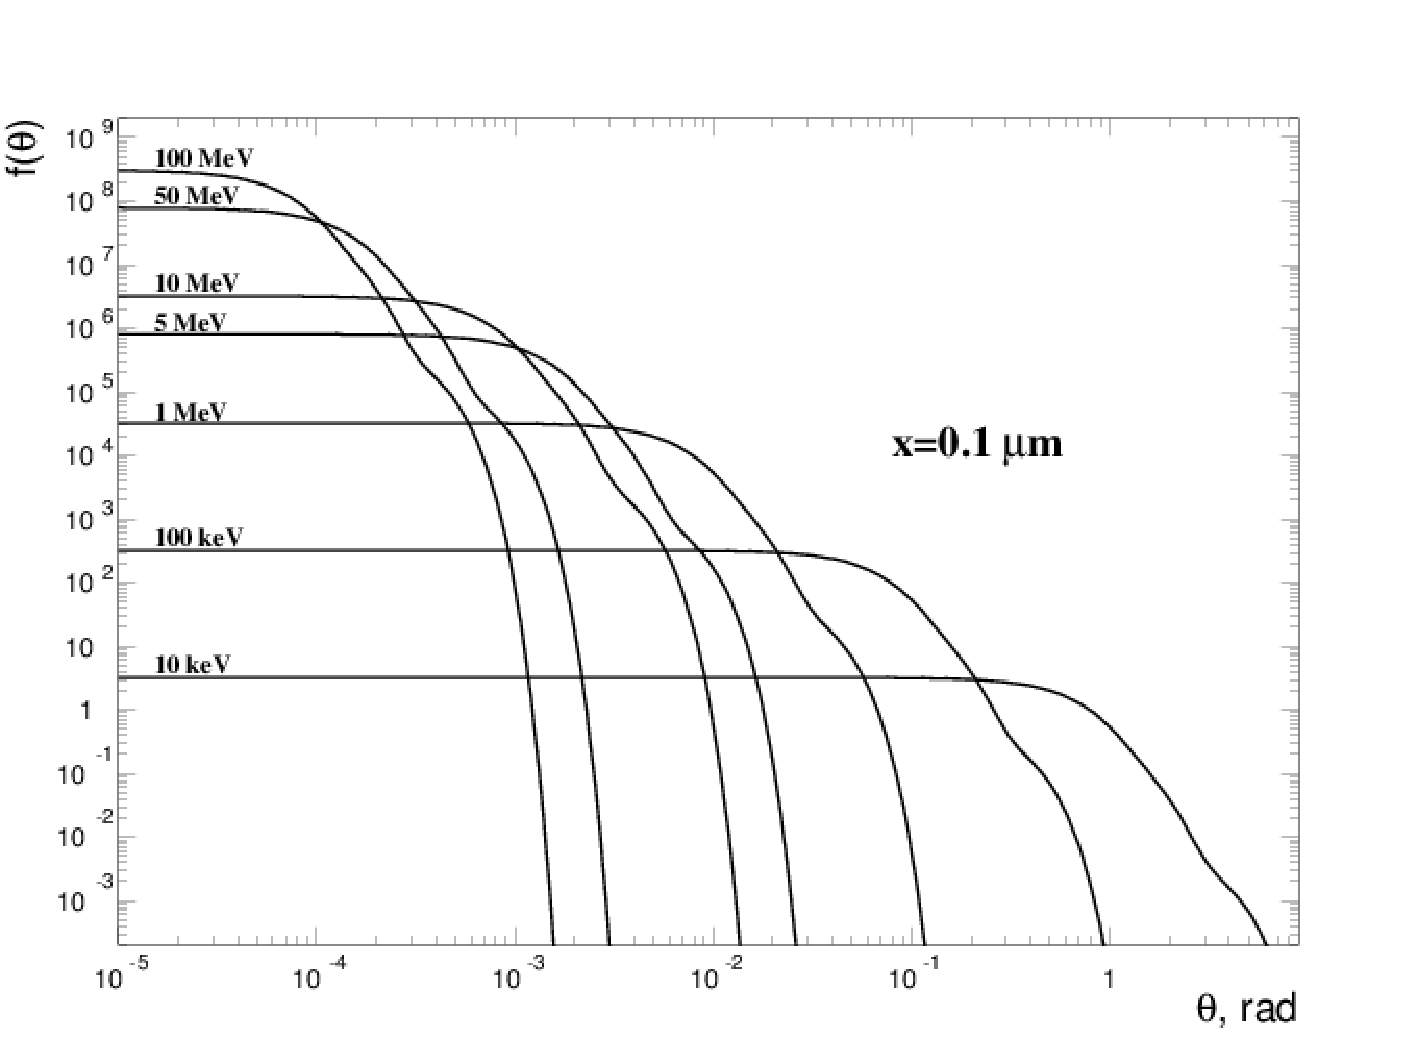
\includegraphics[width=0.32\linewidth]{images/funtheta_0_1mkm_deuteron.pdf}
   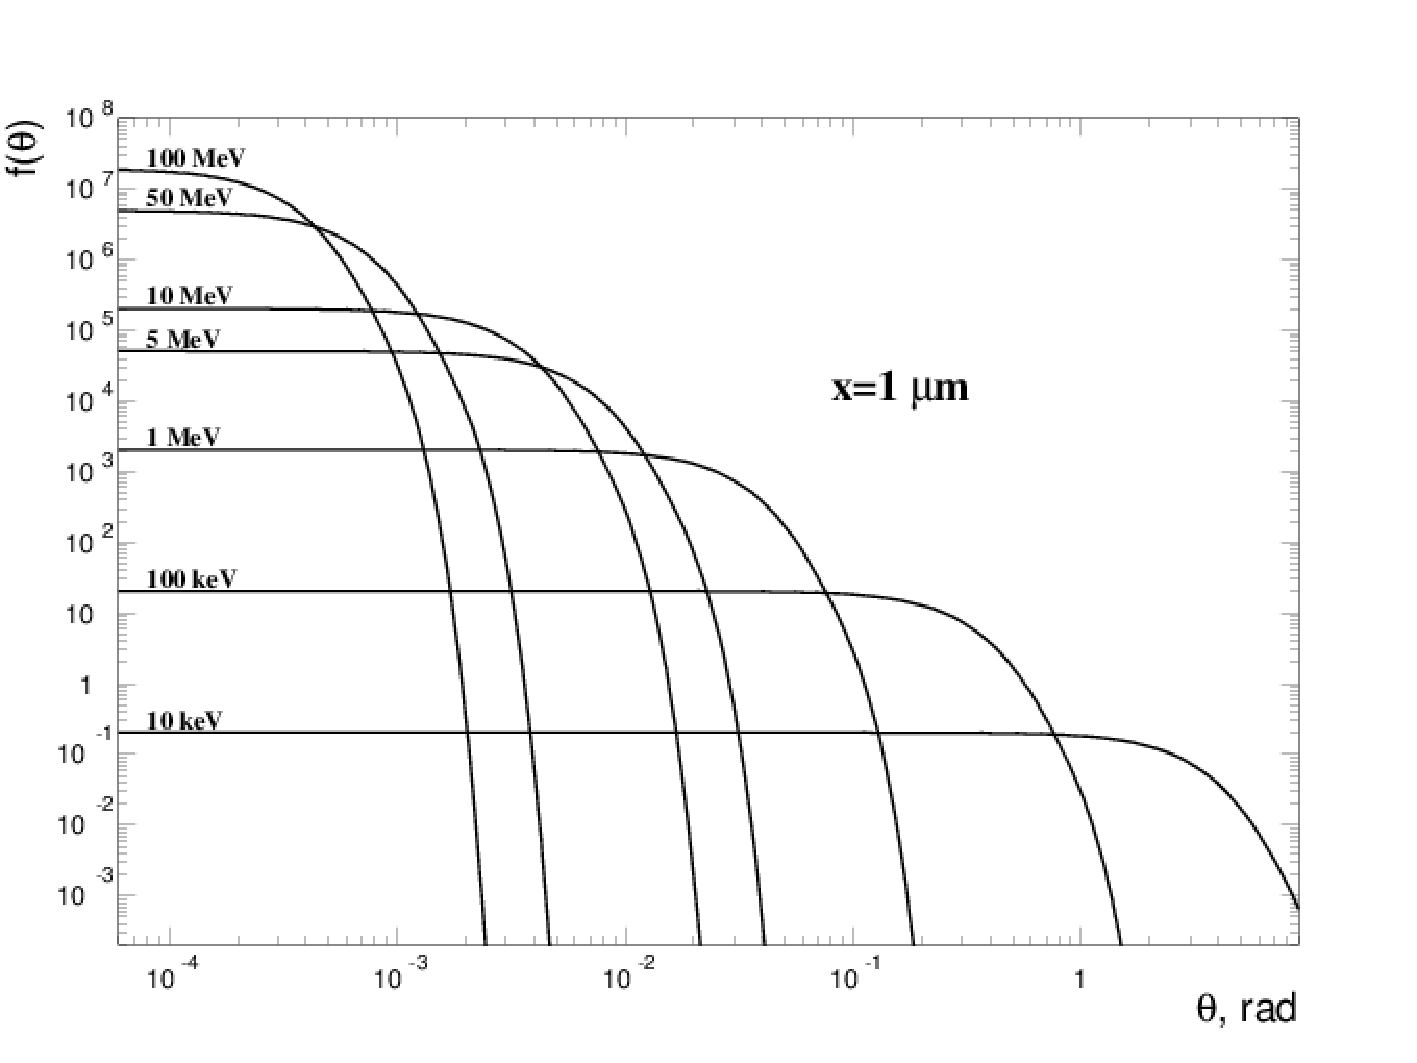
\includegraphics[width=0.32\linewidth]{images/funtheta_1mkm_deuteron.pdf}
   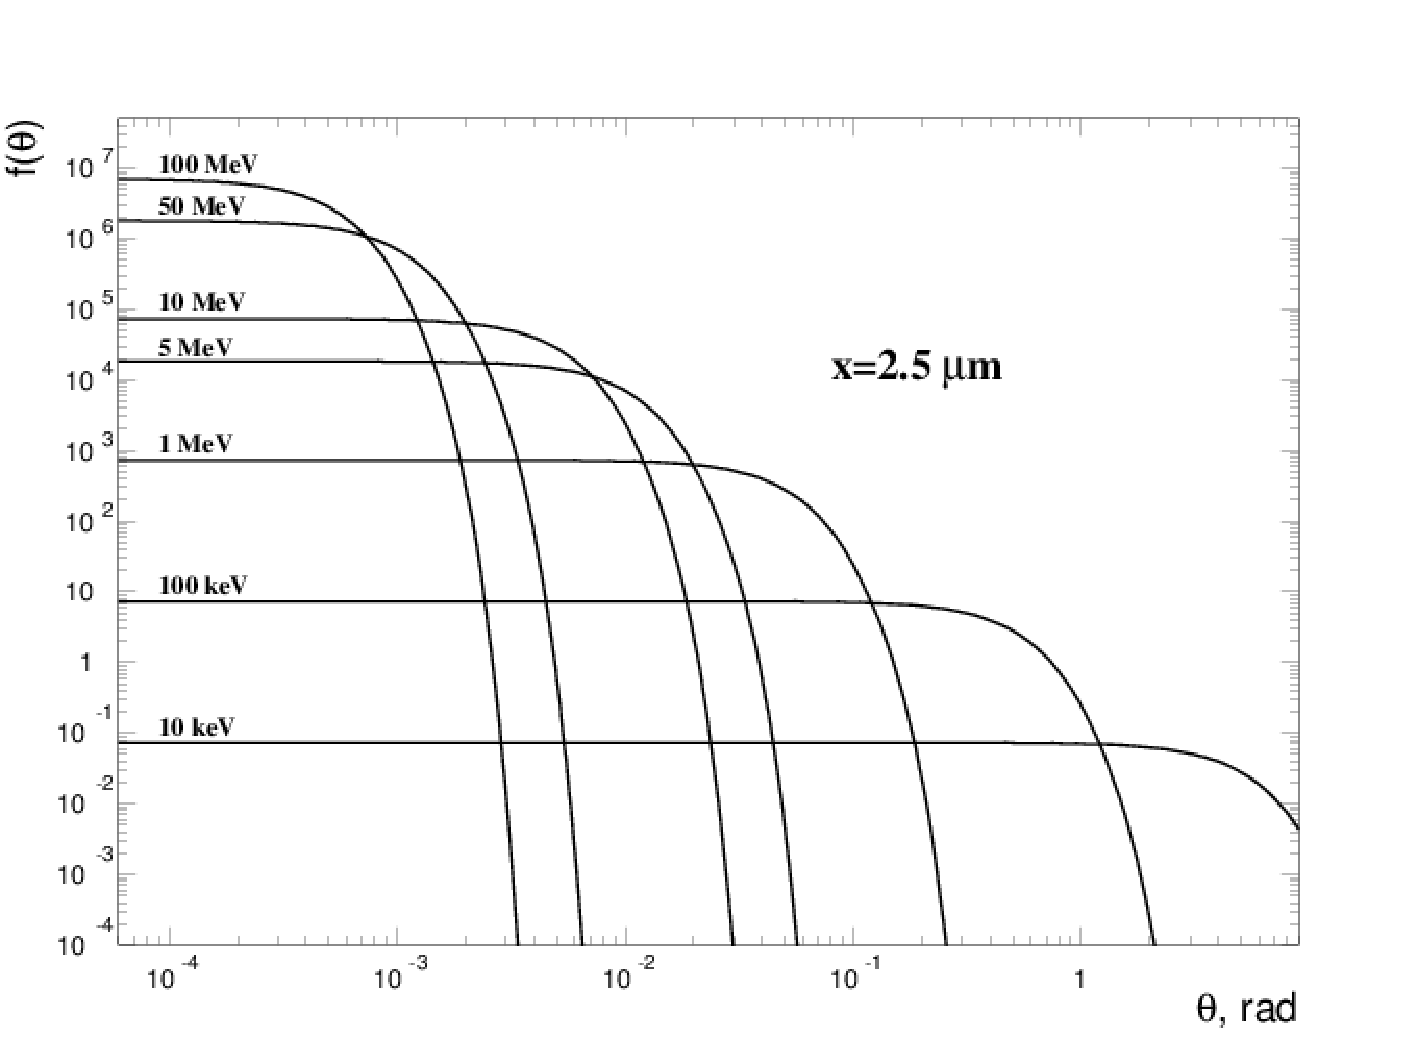
\includegraphics[width=0.32\linewidth]{images/funtheta_2_5mkm_deuteron.pdf}
}
\caption{Пересчёт (скейлинг) полученной для дейтерия с кинетической энергией 10 МэВ в дейтериде титана аппроксимации функции плотности вероятности углового распределения многократного рассеяния $f(\theta,x)$ для произвольных кинетических энергий налетающего иона дейтерия.
	Показаны зависимости при 3 длинах пробега дейтронов в рассеивающей среде мишени: 0.1 $\mu$м, 1 $\mu$м и 2.5 $\mu$м.}
\label{fig:MFthetaScalingDeuteron}
\end{figure}

\begin{figure}[ht]
{
   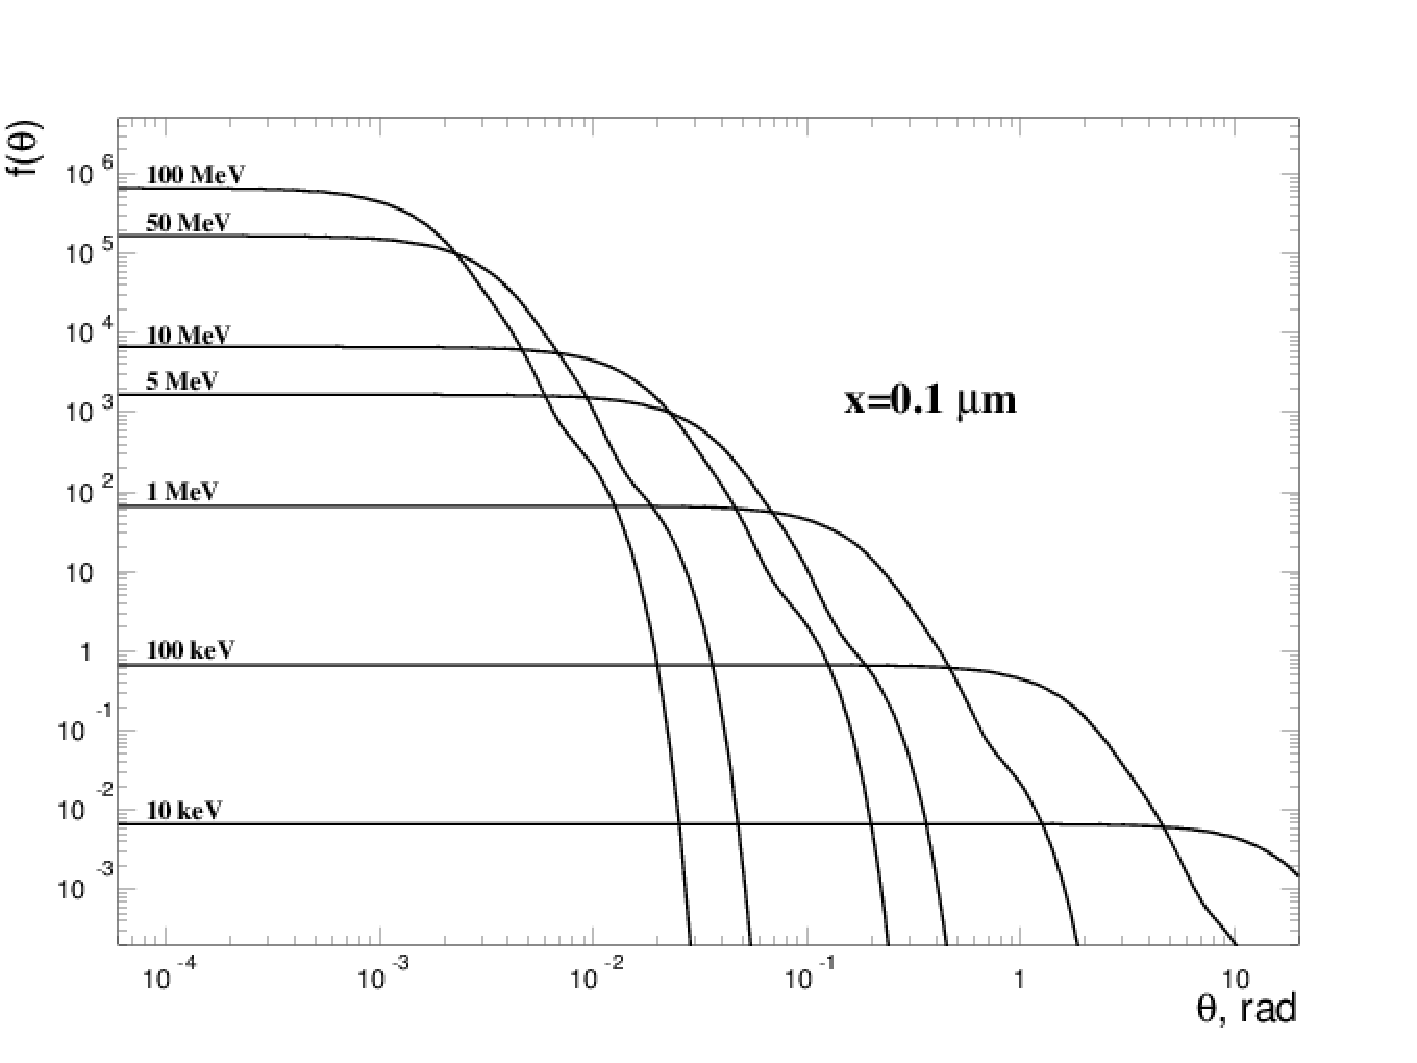
\includegraphics[width=0.32\linewidth]{images/funtheta_0_1mkm_ti.pdf}
   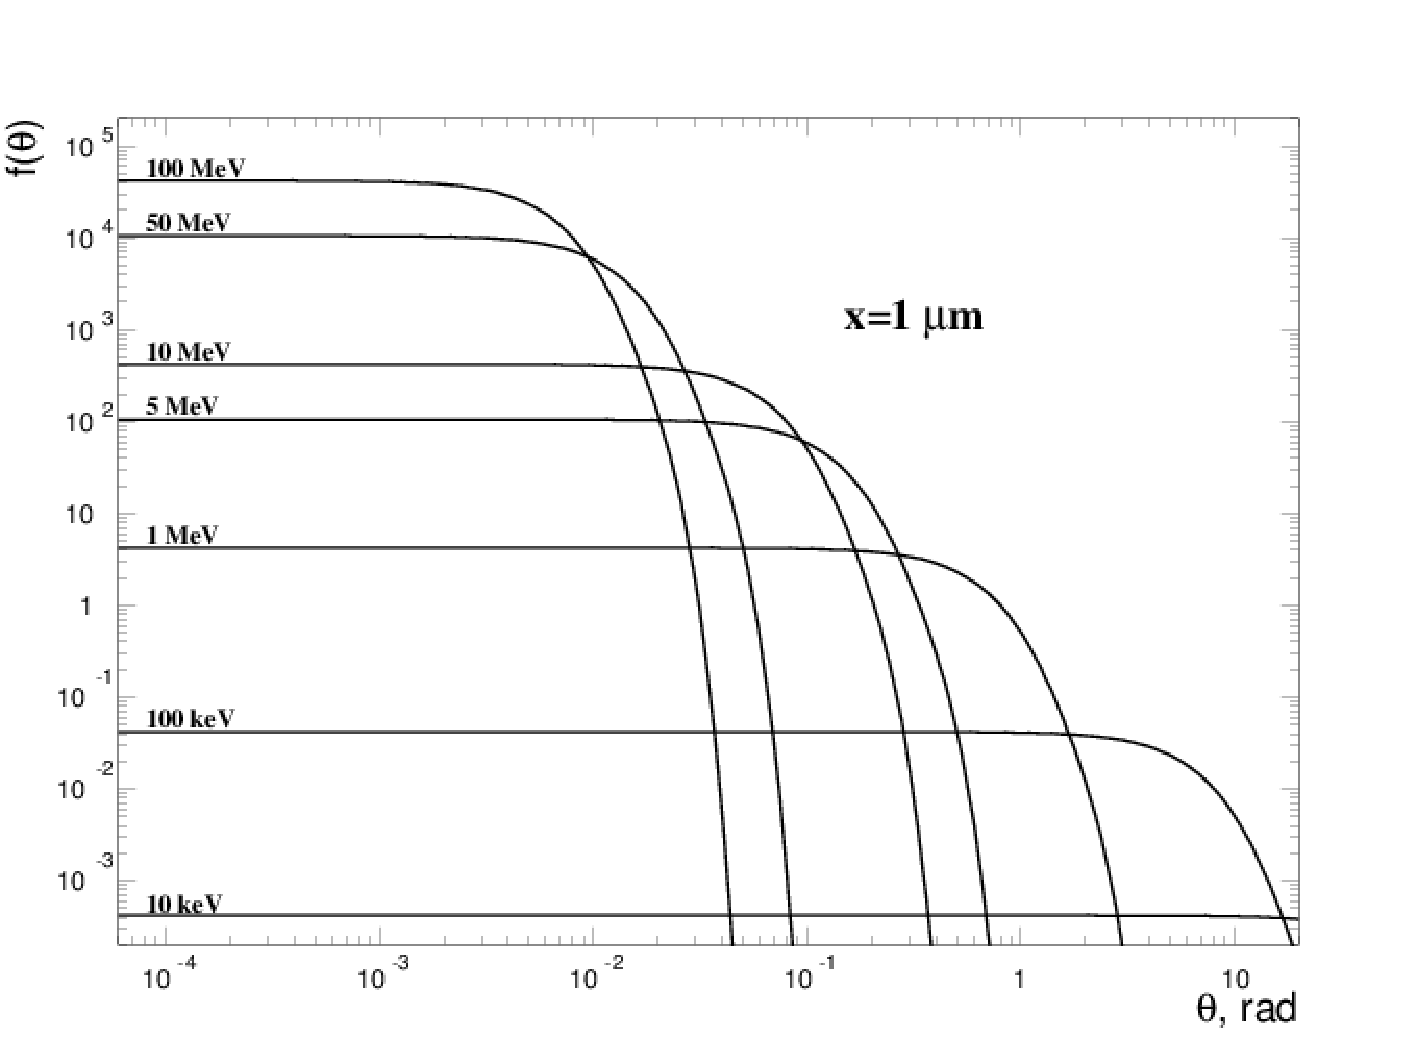
\includegraphics[width=0.32\linewidth]{images/funtheta_1mkm_ti.pdf}
   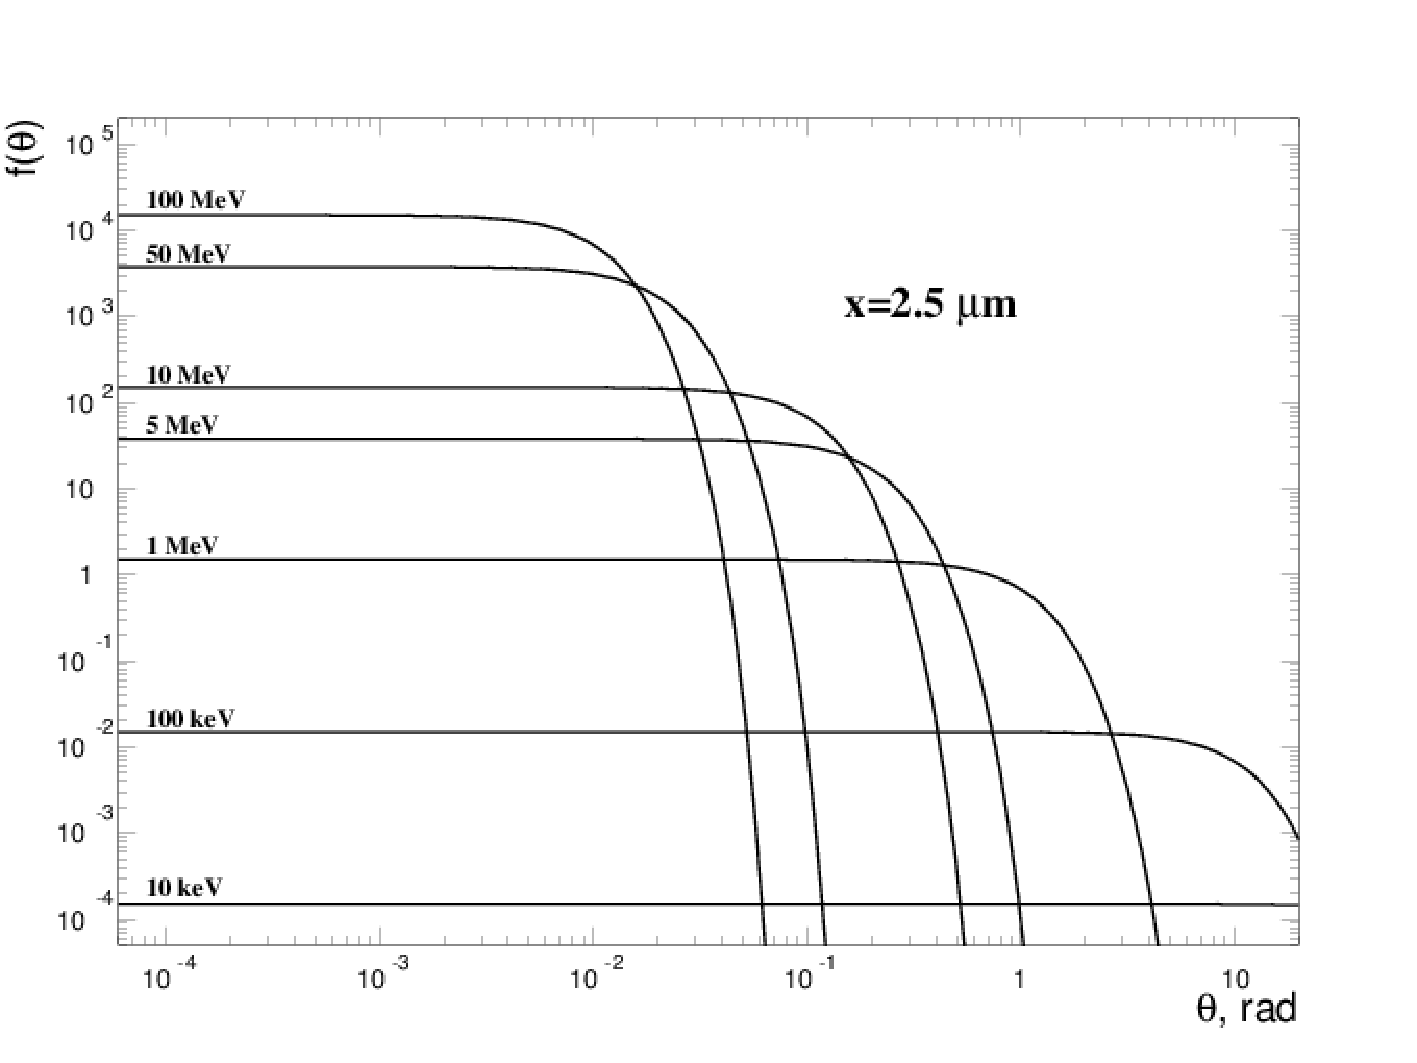
\includegraphics[width=0.32\linewidth]{images/funtheta_2_5mkm_ti.pdf}
}
\caption{Пересчёт (скейлинг) полученной для дейтерия с кинетической энергией 10 МэВ в дейтериде титана аппроксимации функции плотности вероятности углового распределения многократного рассеяния $f(\theta,x)$ для произвольных кинетических энергий налетающего иона титана.
	Показаны зависимости при 3 длинах пробега ионов титана в рассеивающей среде мишени: 0.1 $\mu$м, 1 $\mu$м и 2.5 $\mu$м.}
\label{fig:MFthetaScalingTitan}
\end{figure}

	Также было необходимо проверить, правильно ли работает генерация случайного угла многократного рассеяния на основе данного распределения с помощью генератора псевдослучайных чисел в процессе моделирования.
	Для проверки бралась полученная аппроксимация (\ref{MSApproximationFunction}) углового распределения многократного рассеяния дейтронов с кинетической энергией 10 МэВ в мишени из дейтерида титана.
	
\subsection{Проверка правильности углового распределения, сгенерированного в параллельном коде.}
\label{subValMS3}

	При интегрировании плотности вероятности (\ref{MSApproximationFunction}) надо вычислять не интеграл $\int\limits_{0}^{\tilde \theta} f(\theta) \cdot d\theta$, а интеграл $\int\limits_{0}^{\tilde \theta} f(\theta) \cdot \theta d\theta$, поскольку $\theta$ имеет смысл полярного угла, а значит интегрировать надо по элементу угловой площади $\theta \cdot d \theta$.
	
	В результате интегрирования (\ref{MSApproximationFunction}) получается выражение:
	
\begin{equation}
\label{MSApproximationFunctionIntegral}
\begin{aligned} 
  \int \limits_0^{\infty} \theta \cdot f(\theta) \cdot d\theta=\sum_{i=1}^{3} \frac{W_i}{D_i} \int \limits_0^{\infty} e^{-\frac{\theta^2}{D_i}} \cdot 2 \theta\cdot d\theta = \sum_{i=1}^{3} W_i.
\end{aligned}
\end{equation}

  	Розыгрыш угла начинается с того, что с помощью случайного числа выбирается одно из гауссовых распределений ($W_i,D_i$), относительные вероятности которых рассчитываются по формуле $\frac{W_i}{\sum_{i=1}^{3}W_i}$.
  
  	Угол для выбранного Гауссова распределения разыгрывается как $\theta=\sqrt{-2D_i\cdot\ln{R}}$, где $R$ -- равномерно распределённое случайное число от 0 до 1, то есть используется функция, обратная к гауссовой экспоненте.
  
 	Таким образом, в полной версии программного кода, использующей эффективное распараллеливание по потокам OpenMP и максимально возможную векторизацию, было запущено $N_P=100$ миллионов дейтронов с начальной кинетической энергией 10 МэВ.
 	Их случайные углы многократного рассеяния записывались в гистограмму из $N_{bin}=100$ бинов с логарифмическим шагом от $\theta_{min}=10^{-4}$ рад до $\theta_{max}=0.05$ рад.
 	Границы бинов определялись как $\theta_i=e^{\ln{\theta_{min}+i \cdot \Delta \ln{\theta}}}$, где логарифмический шаг по оси $\theta$ есть $\Delta \ln{\theta}=\frac{\ln{\theta_{max}}-\ln{\theta_{min}}}{N_{bin}-1}$.
 	В итоге получались $N_{bin}$ величин $\Delta N_i$, соответствующих числу событий в каждом из $N_{bin}$ логарифмических бинов.
 	Эти величины $\Delta N_i$ для нормировки (функция плотности вероятности (\ref{MSApproximationFunction}) нормирована на 1 частицу) делились на полное число частиц, равное $N_P$, и на величину $\theta_i^2 \cdot \Delta \ln{\theta}=\theta_i \cdot \Delta \theta_i$, соответствующую малому элементу угловой площади, где величина $\theta^{mid}_i$ бралась в среднегеометрической середине бина, равной $\theta^{mid}_i=\sqrt{ \theta_i \cdot \theta_{i+1}}$ при $i$, изменяющемся от 0 до $N_{bin}-1$.
 	Получалась величина $f(\theta_i)=\frac{1}{N_P} \cdot \frac{\Delta N_i}{\Delta\ln{\theta} \cdot \theta^2_i}=\frac{1}{N_P} \cdot \frac{\Delta N_i}{\theta_i \cdot \Delta \theta_i}$.
  
 	В итоге были выбраны 6 значений пробега, пройденного потоком из $N_P$ частиц, в веществе, и для каждого из них построены гистограммы отношения полученной в ходе моделирования $f(\theta_i,x)$ к точно вычисленному по найденной аппроксимации (\ref{MSApproximationFunction}) в среднегеометрической середине логарифмического бина $\theta^{mid}_i$ значению функции плотности верятности углового распределения многократного рассеяния.
 	Результат изображён на Рис. ~\ref{fig:MSRatioHistogramWithoutCorrection}.
 	
\begin{figure}[ht]
{
   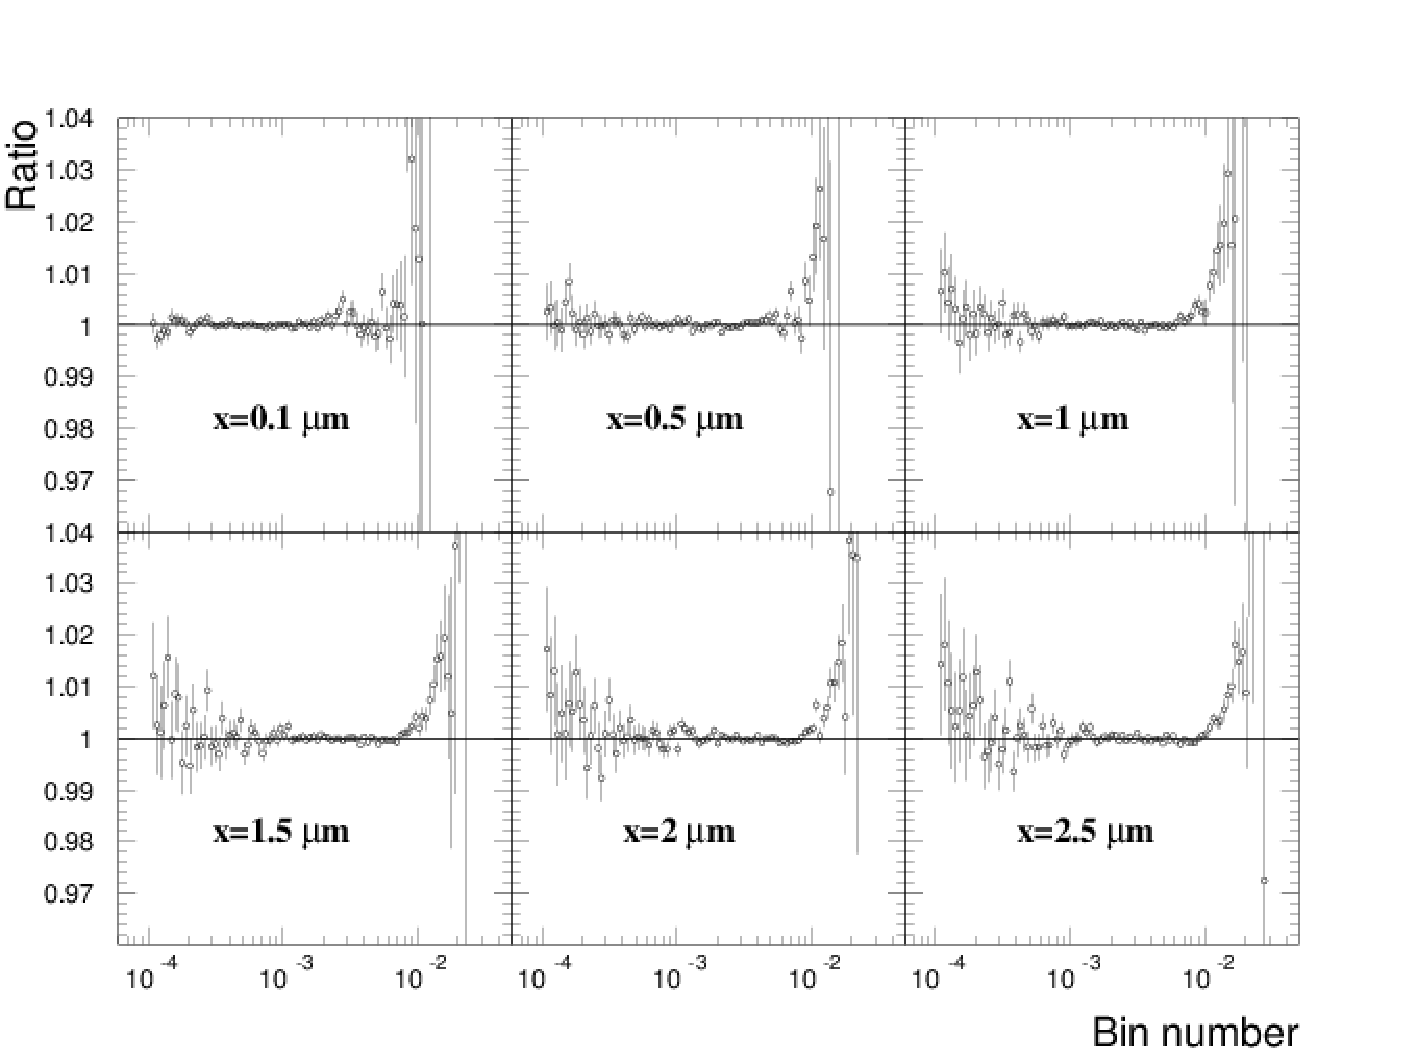
\includegraphics[width=0.99\linewidth]{images/ratioms_without_correction.pdf}
}
\caption{Отношение полученной в ходе моделирования $f(\theta_i)$ к точно вычисленному по найденной аппроксимации (\ref{MSApproximationFunction}) в среднегеометрической середине логарифмического бина $\theta^{mid}_i$ значению функции плотности верятности углового распределения многократного рассеяния.}
\label{fig:MSRatioHistogramWithoutCorrection}
\end{figure}

	Из Рис. ~\ref{fig:MSRatioHistogramWithoutCorrection} видно, что в целом отношение близко к 1 с очень хорошей точностью, но при приближении к правой границе гистограммы наблюдается его явный рост.
	Было выяснено, что этот рост связан с тем, что логарифмические бины гистограммы растут слева направо, у правой границы гистограммы их размер сильно возрастает.
	В то же время функция (в (\ref{MSApproximationFunction}) входят 3 гауссоиды, но без ограничения общности для простоты можно рассматривать 1 распределение Гаусса) распределения Гаусса является сильно падающей.
	Поэтому то, какому значению $\theta$ в каждом бине соответсвует полученное в ходе моделирования $f(\theta_i)$, нужно находить интегрированием, в то время как у нас берётся среднегеометрическая середина бина $\theta^{mid}_i$.
	Наблюдающийся рост отношения свидетельствует о том, что в правых бинах гистограммы ``среднее'' рассчитанное путём интегрирования значение $\theta$ лежит левее $\theta^{mid}_i$, а мы как бы завышаем это значение $\theta$, тем самым занижая значение $f(\theta_i)$, чем и объясняется загиб вверх отношения у правой границы гистограммы. Подробные выкладки приводятся ниже.
  
\subsection{Коррекция углового распределения, сгенерированного в параллельном коде, в связи с логарифмической шкалой гистограммы и сильно падающей функцией распределения Гаусса.}
\label{subValMS4}

	Если проинтегрировать функцию распределения Гаусса $F(\theta)=C \cdot \frac{2}{D} \cdot e^{-\frac{\theta^2}{D}}$, где нормировочный коэффициент $C$ мы в дальнейшем опустим, по угловой площади $\theta \cdot d\theta$ в пределах заданного бина (здесь рассматривается линейный масштаб, но аналогичные выкладки можно провести и в логарифмическом масштабе, проводя интегрирование по оси $\ln{\theta}$, которая в этом случае будет линейна), чтобы получить среднее значение функции $F(\theta)$ в этом бине, получится
\begin{equation}
\label{MSIntegralExp}
\begin{aligned} 
  \langle f \rangle = \frac{1}{2\Delta} \cdot \int \limits_{\theta_{mid} - \Delta}^{\theta_{mid} + \Delta} \theta \cdot F(\theta) \cdot d \theta =
  \frac{e^{-\frac{\left( \theta_{mid} - \Delta \right)^2}{D}} - e^{-\frac{\left( \theta_{mid} + \Delta \right)^2}{D}}}{2\Delta} = \\
  e^{-\frac{\theta^2_{mid} + \Delta^2}{D}} \cdot \frac{ e^{\frac{2 \cdot \theta_{mid} \cdot \Delta}{D}} - e^{-\frac{2 \cdot \theta_{mid} \cdot \Delta}{D}} }{2\Delta},
\end{aligned}
\end{equation}
	где $\Delta$ -- полуширина бина, а $\theta_{mid}$ -- его середина.

	Если воспользоваться разложением экспоненты в ряд по малому параметру $\frac{2 \cdot \theta_{mid} \cdot \Delta}{D}$, можно получить, что
\begin{equation}
\label{MSIntegralExpand}
\begin{aligned} 
  \frac{ e^{\frac{2 \cdot \theta_{mid} \cdot \Delta}{D}} - e^{-\frac{2 \cdot \theta_{mid} \cdot \Delta}{D}} }{2\Delta} =
  \frac{2 \cdot \theta_{mid}}{D}.
\end{aligned}
\end{equation}
	Т. к. $\frac{2 \cdot \theta_{mid} \cdot \Delta}{D}$ -- малый параметр, то раскладываем экспоненту только до 1-го порядка малости, чётные степени сокращаются, а нечётные высших порядков не вносят вклада из-за малости параметра.

	В итоге выражение (\ref{MSIntegralExp}) принимает вид
\begin{equation}
\label{MSIntegralFin}
\begin{aligned} 
  \langle f \rangle = \frac{2}{D} \cdot e^{-\frac{\theta^2_{mid}}{D}} \cdot \theta_{mid} \cdot e^{-\frac{\Delta^2}{D}} .
\end{aligned}
\end{equation}

	В нём первое слагаемое $\frac{2}{D} \cdot e^{-\frac{\theta^2_{mid}}{D}}$ с точностью до нормировочного коэффициента соответствует точному значению функции аппроксимации углового распределения многократного рассеяния, рассчитанному в середине бина $\theta_{mid}$, а множитель $\theta_{mid} \cdot e^{-\frac{\Delta^2}{D}}$ как раз и отвечает за загиб вверх в правой части гистограммы на Рис. ~\ref{fig:MSRatioHistogramWithoutCorrection}.
	
	Поэтому, если скорректировать полученные в результате моделирования значения $f(\theta_i)$, поделив их на $\theta_{mid} \cdot e^{-\frac{\Delta^2}{D}}$, рост в правой части гистограммы на Рис. ~\ref{fig:MSRatioHistogramWithoutCorrection} должен исчезнуть.
	Результат показан на Рис. ~\ref{fig:MSRatioHistogramWithCorrection}.
	Как видно, аномальный рост исчез, и отношение в пределах погрешности равно 1.
	
\begin{figure}[ht]
{
   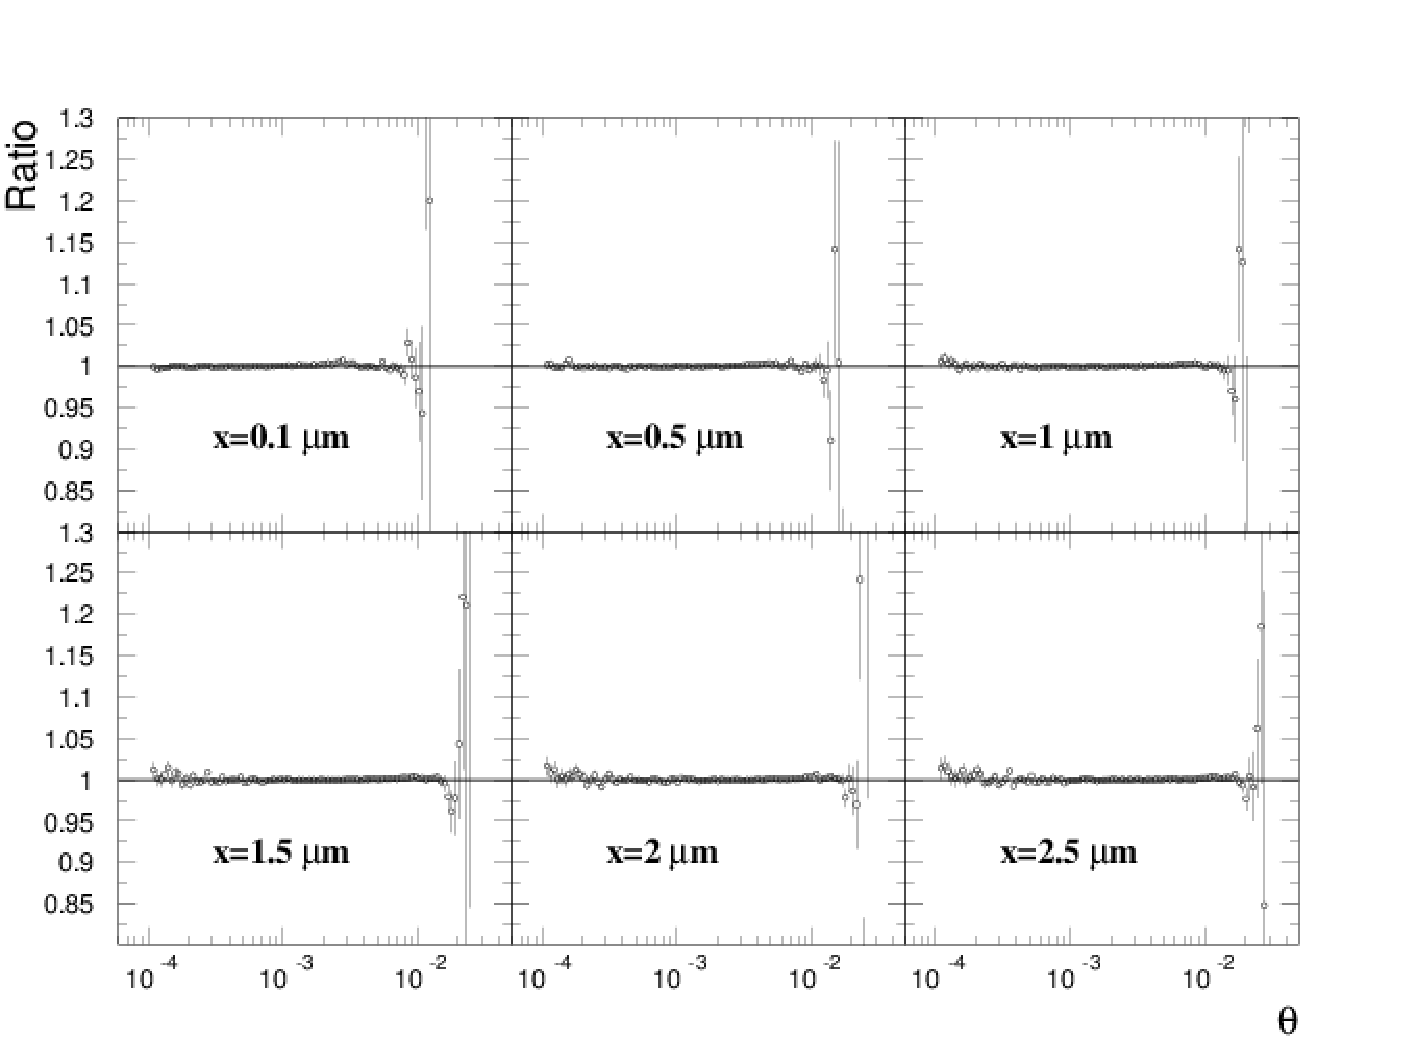
\includegraphics[width=0.99\linewidth]{images/ratioms_with_correction.pdf}
}
\caption{Отношение полученной в ходе моделирования $f(\theta_i)$ \underline{после коррекции} к точно вычисленному по найденной аппроксимации (\ref{MSApproximationFunction}) в среднегеометрической середине логарифмического бина $\theta^{mid}_i$ значению функции плотности вероятности углового распределения многократного рассеяния.}
\label{fig:MSRatioHistogramWithCorrection}
\end{figure}

	Как видно из выражения (\ref{MSIntegralFin}), данная коррекция необходима и при линейное шкале, когда $\Delta=const$, но при логарифмической шкале $\Delta$ сильно растёт справа налево оси $x$, и коэффициент коррекции гораздо больше.
	Независимо от шкалы присутствует коэффициент $\theta_{mid}$, который необходимо корректировать.

	Таким образом, было показано, что многократное рассеяние можно успешно моделировать в параллельном и векторизованном программном коде при помощи полученной аппроксимации его углового распределения (\ref{MSApproximationFunction}).
	
	
\clearpage{}
\section{Валидация углового распределения неупругой D-D реакции.}
\label{ValInelasticDD}

	Для моделирования ионного каскада в мишени из дейтерида титана, вызванного облучением мишени интенсивным потоком дейтронов, необходимо знать интегральное сечение и угловое распределение неупругой D-D реакции. 
	
	Экспериментальные данные интегральных сечений обоих каналов (p+t и n+$^3_2$He) брались из базы данных ENDF-6 и аппроксимировались дробно-рациональными функциями.
	В результате чего были получены функции зависимости интегрального сечения каждого из выходных каналов неупругой D-D реакции от кинетической энергии налетающего дейтрона в системе центра масс $T_{CM}$, равной для случая рассеяния одинаковых частиц половине кинетической энергии налетающей частицы в лабораторной системе $T_{LS}$:
	
\begin{equation}
\label{InelasticDDNHe3ChannelIntegralCrossSection}
\begin{aligned} 
  \sigma^{n+^3_2He}(T_{CM}) = \frac{0.21}{\left( 1 + \left(\frac{2.52\cdot 10^{-2}}{T_{CM}} \right)^{1.5} \right) \cdot \left( 1 + \left( \frac{4.7\cdot 10^{-3}}{T_{CM}} \right)^{4.5} \right) \cdot \left( 1+0.23 \cdot T_{CM} \right) } \cdot g
\end{aligned}
\end{equation}

и

\begin{equation}
\label{InelasticDDPTChannelIntegralCrossSection}
\begin{aligned} 
  \sigma^{p+t}(T_{CM}) = \frac{0.176}{\left( 1 + \left(\frac{2\cdot 10^{-2}}{T_{CM}} \right)^{1.7} \right) \cdot \left( 1.0 + \left( \frac{4.3\cdot 10^{-3}}{T_{CM}} \right)^{4.4} \right) \cdot \left( 1+\left( 0.17 \cdot T_{CM} \right)^{0.85} \right) } \cdot g,
\end{aligned}
\end{equation}
	
	где фактор Гамова есть $g=e^{-\frac{1}{2}\sqrt{\frac{Eg}{T_{CM}}}}$, а $E_g$ -- энергия Гамова, равная для D-D рассеяния 0.986 МэВ.
	На Рис. ~\ref{fig:InelasticDDIntegralCrossSections} изображены выражения (\ref{InelasticDDNHe3ChannelIntegralCrossSection}) и (\ref{InelasticDDPTChannelIntegralCrossSection}), делённые на фактор Гамова.
	Они определяют величину сечений соответствующих каналов реакции в барнах.
	
\begin{figure}[ht]
  {
     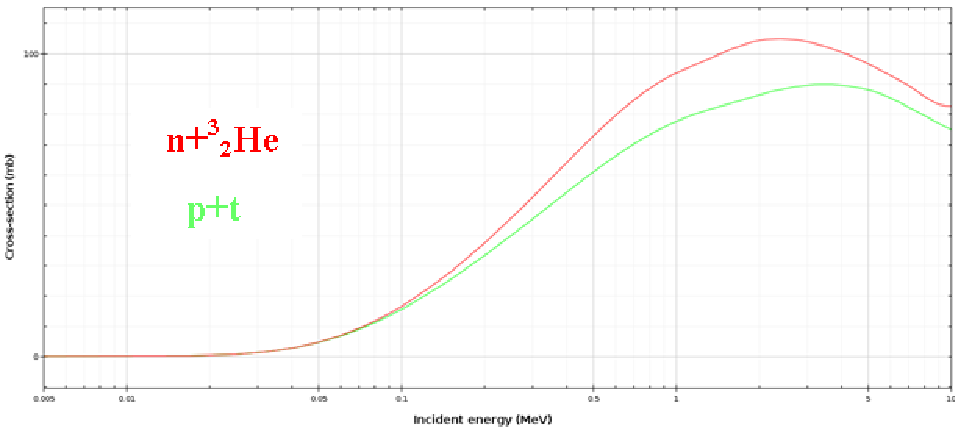
\includegraphics[width=0.99\linewidth]{images/DDInelasticIntegralCrossSections.pdf}
  }
  \caption{Зависимость интегральных сечений каналов неупругой D-D реакции от кинетической энергии в системе центра масс $T_{CM}$.}
  \label{fig:InelasticDDIntegralCrossSections}
\end{figure}	
	
	
	Угловые распределения неупругой D-D реакции брались из базы данных TPT2 в виде нормированных частичных сумм от -1 до 1 по $\cos{ \left( \theta_{CM} \right) }$.
	В базе данных ТРТ2 записаны нормированные частичные суммы для каждого из 67 значений кинетической энергии от $10^{-4}$ МэВ до 10 МэВ с линейным шагом.
	Эти 67 наборов энергий и частичных сумм читались из базы данных ТРТ2, и с помощью линейной интерполяции из них получалась более подробная база данных частичных сумм для 512 значений кинетической энергии налетающего дейтрона с линейным шагом в том же диапазоне.
	Из них с помощью бинарного поиска по кинетической энергии $T_{LS}$ налетающего дейтрона, случайных чисел и квадратичной интерполяции получались значения $\cos{ \left( \theta_{CM} \right) }$ в ходе моделирования.
	Квадратичная интерполяция использовалась для более точного описания углового распределения.
	Ведь если использовать линейную интерполяцию, это приведёт к тому, что угловое распределение, сгенерированное с помощью случайных чисел, будет ступенчатым, а при использовании квадратичной интерполяции сгенерированное угловое распределение будет сплайном 2 порядка, проходящим по точкам, соответствующим значениям частичных сумм.
	
	Нужно было проверить правильность сгенерированного в ходе моделирования с помощью разрабатываемого параллельного программного кода TPT3 углового распределения неупругой реакции D+D.
	Т. к. нормализованные частичные суммы, записанные в базу данных ТРТ2, получены интегрированием полиномов Лежандра, коэффициенты разложения дифференциального сечения неупругой D-D реакции по которым заданы в базе ENDF-6, из-за сложности полиномов Лежандра, очевидно, не представляется возможным получить аналитическую функцию, с помощью которой можно было бы провести нужное сравнение.
	Поэтому было проведено моделирование неупругой D-D реакции в тонкой мишени с помощью Geant4.
	В ходе моделирования запускалось 2 миллиарда дейтронов и с помощью программного пакета ROOT заполнялись гистограммы нормированного углового распределения продуктов реакции при различных кинетических энергиях налетающих дейтронов.
	Данные гистограммы нормированного дифференциального сечения сравнивались с полученными при моделировании разрабатываемым параллельным программным кодом TPT3 при нескольких значениях кинетической энергии налетающего дейтрона в лабораторной системе, и при всех этих значениях кинетической энергии получилось отличное совпадение с расхождением не более 1 \% результатов моделирования Geant4 и разрабатываемым программным кодом, работающим и на CPU, и на GPU.
	Например, при кинетической энергии налетающего дейтрона, равной 2 МэВ, соотношение результатов моделирования изображено на  Рис. ~\ref{fig:ValidationThermonuclear2mev2billionParticles}.
	
\begin{figure}[ht]
  {
     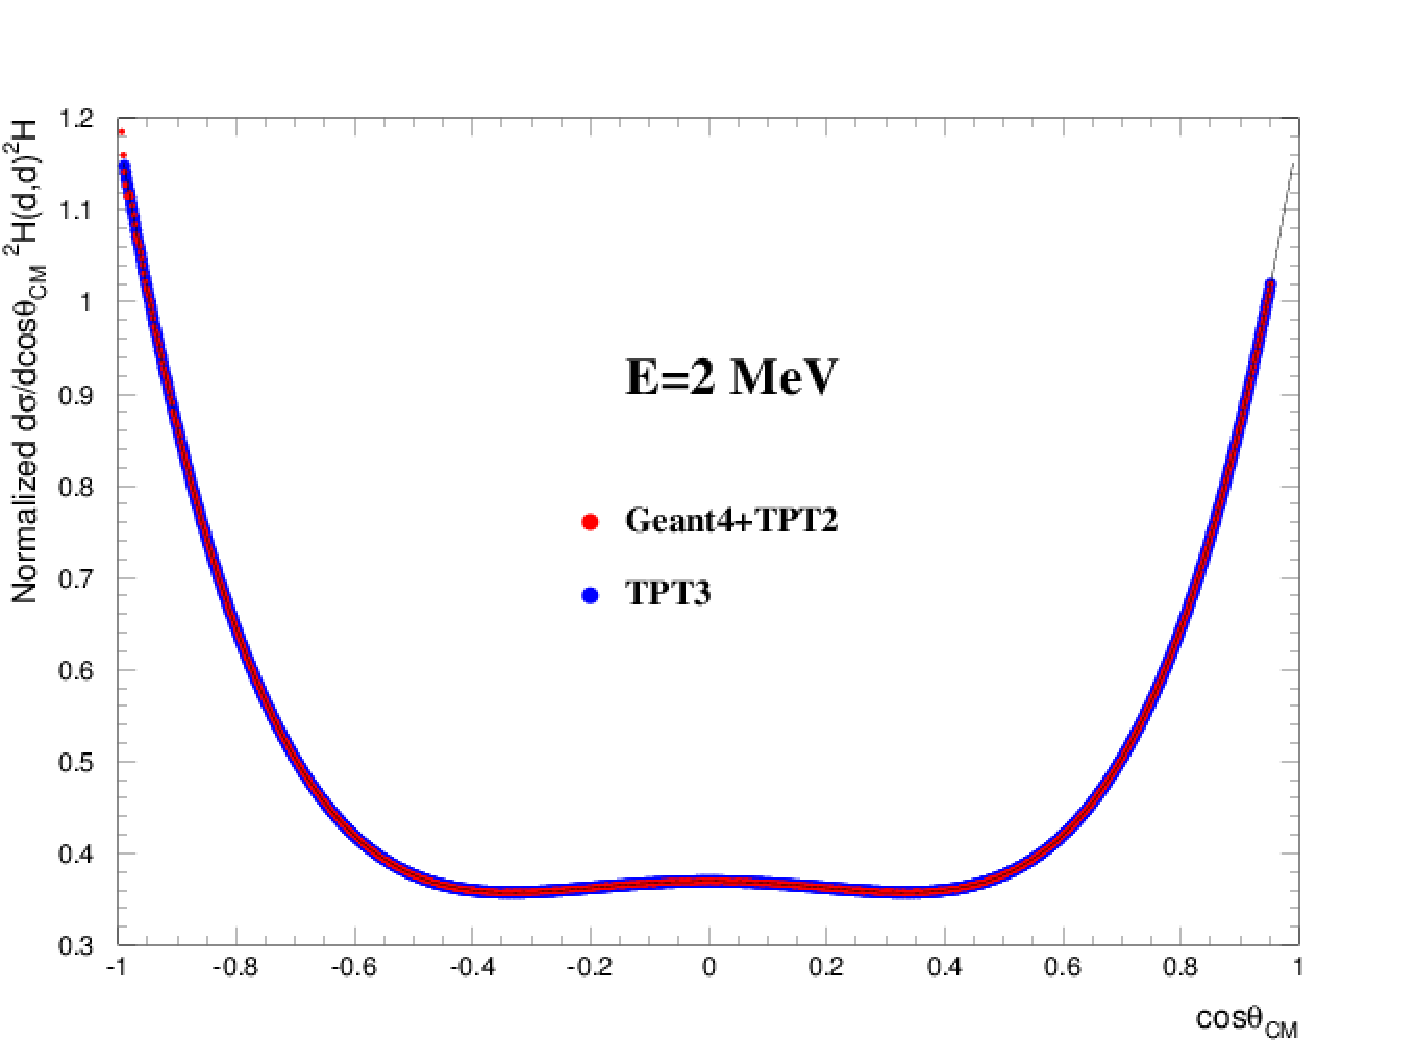
\includegraphics[width=0.99\linewidth]{images/validation_thermonuclear_2mev_2billion.pdf}
  }
  \caption{Сравнение гистограмм нормированного дифференциального сечения, полученных при моделировании неупругой D-D реакции в тонкой мишени дейтерида титана при запуске 2 миллиардов дейтронов с помощью Geant4 и разрабатываемого параллельного программного кода TPT3.}
  \label{fig:ValidationThermonuclear2mev2billionParticles}
\end{figure}	
	
	Некоторое отличие между результатами моделирования наблюдается в области обратного рассеяния около    $\cos{ \left( \theta_{CM} \right) }=-1$.
	Оно показано на Рис. ~\ref{fig:CompareTPT2WithTPT32billionParticles}.
	Как выяснилось, это вызвано тем, что в области $\cos{ \left( \theta_{CM} \right) }=1$ частичные суммы очень мало отличаются от единицы и друг от друга.
	Чтобы увеличить это отличие и для удобства моделирования, в базу данных TPT2 записывались не частичные суммы, а квадратный корень из них.
	Но тогда при розыгрыше $\cos{ \left( \theta_{CM} \right) }$ с помощью случайного числа нужно было брать корень из случайного числа, но в программном комплексе TPT2 бралось случайное число, а не его корень. Это и было причиной ошибки.
	Как видно из Рис. ~\ref{fig:CompareTPT2WithTPT32billionParticles}, этот баг TPT2 исправлен в TPT3. 		И если не рассматривать эту малую область при $\cos{ \left( \theta_{CM} \right) }=-1$, результаты моделирования Geant4 и разрабатываемым параллельным программным комплексом TPT3, везде совпадают с отличной точностью.
	
\begin{figure}[ht]
  {
     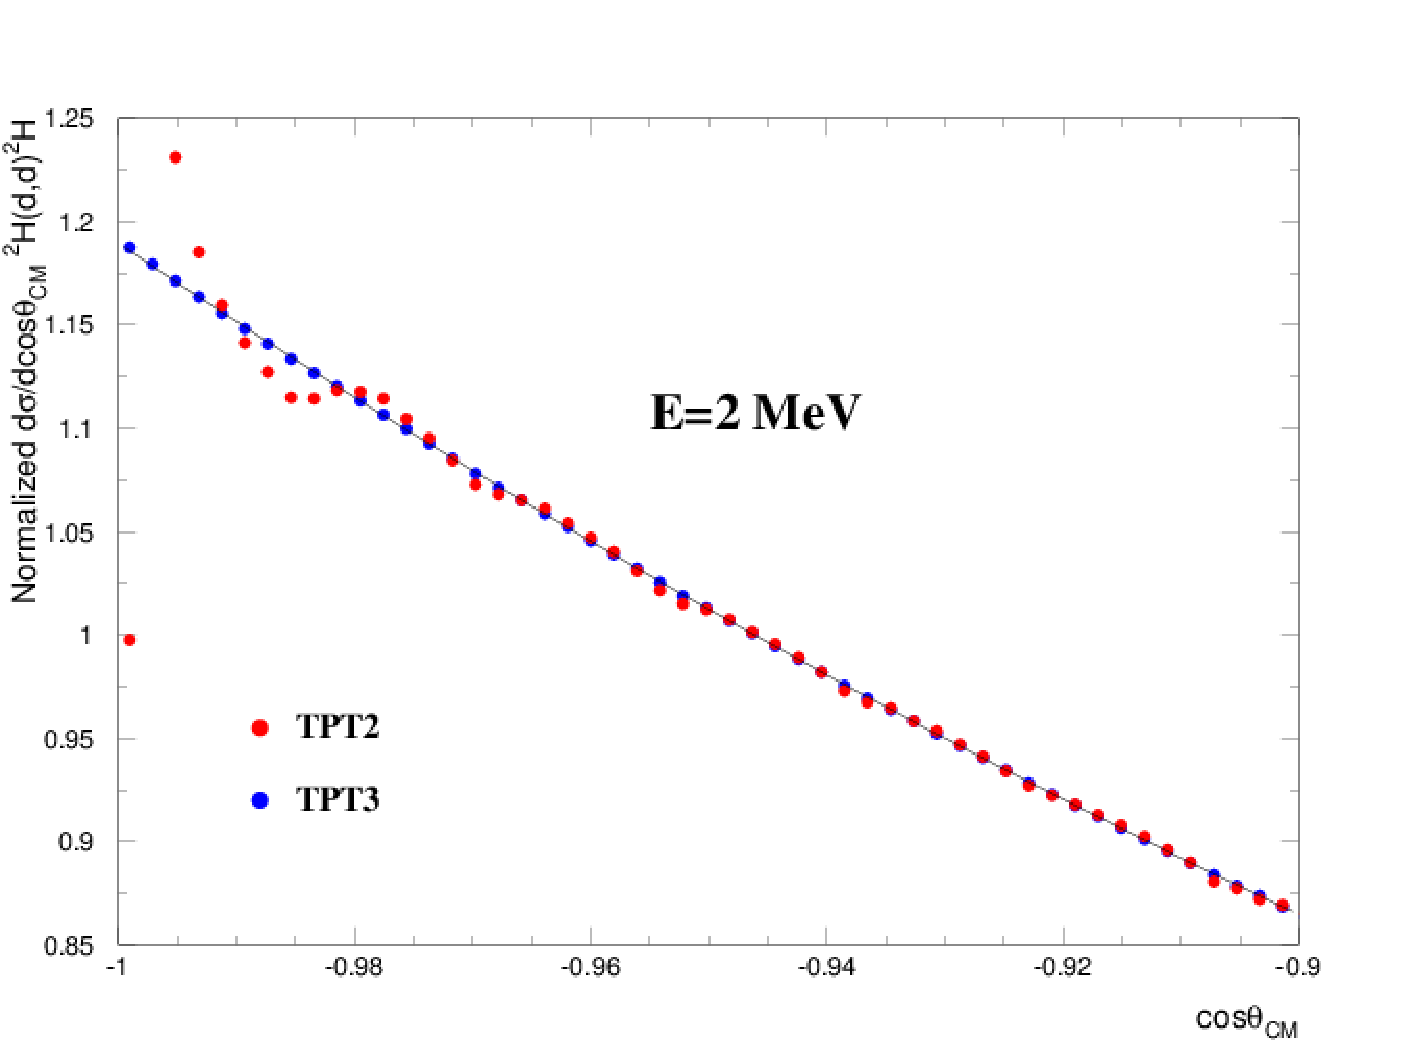
\includegraphics[width=0.99\linewidth]{images/compare_tpt2_with_tpt3_2billion.pdf}
  }
  \caption{Отличие результатов моделирования с помощью Geant4 и с помощью разрабатываемого параллельного программного кода TPT3 неупругой D-D реакции в тонкой мишени дейтерида титана в районе $\cos{ \left( \theta_{CM} \right) }=-1$ при запуске 2 миллиардов дейтронов.}
  \label{fig:CompareTPT2WithTPT32billionParticles}
\end{figure}	
	

\clearpage{}
\section{Валидация углового распределения упругого D-D рассеяния.}
\label{ValElasticDD}
\
	Для моделирования ионного каскада в мишени из дейтерида титана, вызванного облучением мишени интенсивным потоком дейтронов, необходимо было также использовать аппроксимацию дифференциального сечения упругого D-D рассеяния, полученную в отчёте \cite{70/778-T}.
	Обычно для моделирования упругого рассеяния из-за кулоновского барьера и ряда других причин используют просто дифференциальное сечение Резерфордовского рассеяния.
	Особенность данной аппроксимации в том, что она получена для интерференции электромагнитной (Резерфордовское рассеяние) и ядерной (сильное взаимодействие) амплитуд рассеяния.
	Отличие от Резерфордовского дифференциального сечения проявляется в области максимального угла рассеяния $\theta_{CM}=\frac{\pi}{2}$ в системе центра масс (т. к. рассеиваются тождественные частицы, угол рассеяния $\theta_{CM}$ изменяется от 0 до $\frac{\pi}{2}$), что показано на Рис. ~\ref{fig:DifferenceOfElasticDDFromRutherfordDifferentialCrossSection}, где углу рассеяния $\theta_{CM}=\frac{\pi}{2}$ соответствует правая часть оси абсцисс, где $\cos{\theta_{CM}}=0$ и $1-\cos{\theta_{CM}}=1$.
	Т. е. отличие полного дифференциального сечения упругого рассеяния от чисто Резерфордовского наблюдается при рассеянии на большие углы.
	Как видно из Рис. ~\ref{fig:DifferenceOfElasticDDFromRutherfordDifferentialCrossSection}, оно существенно, и его необходимо учитывать при моделировании.
	
\begin{figure}[ht]
  {
     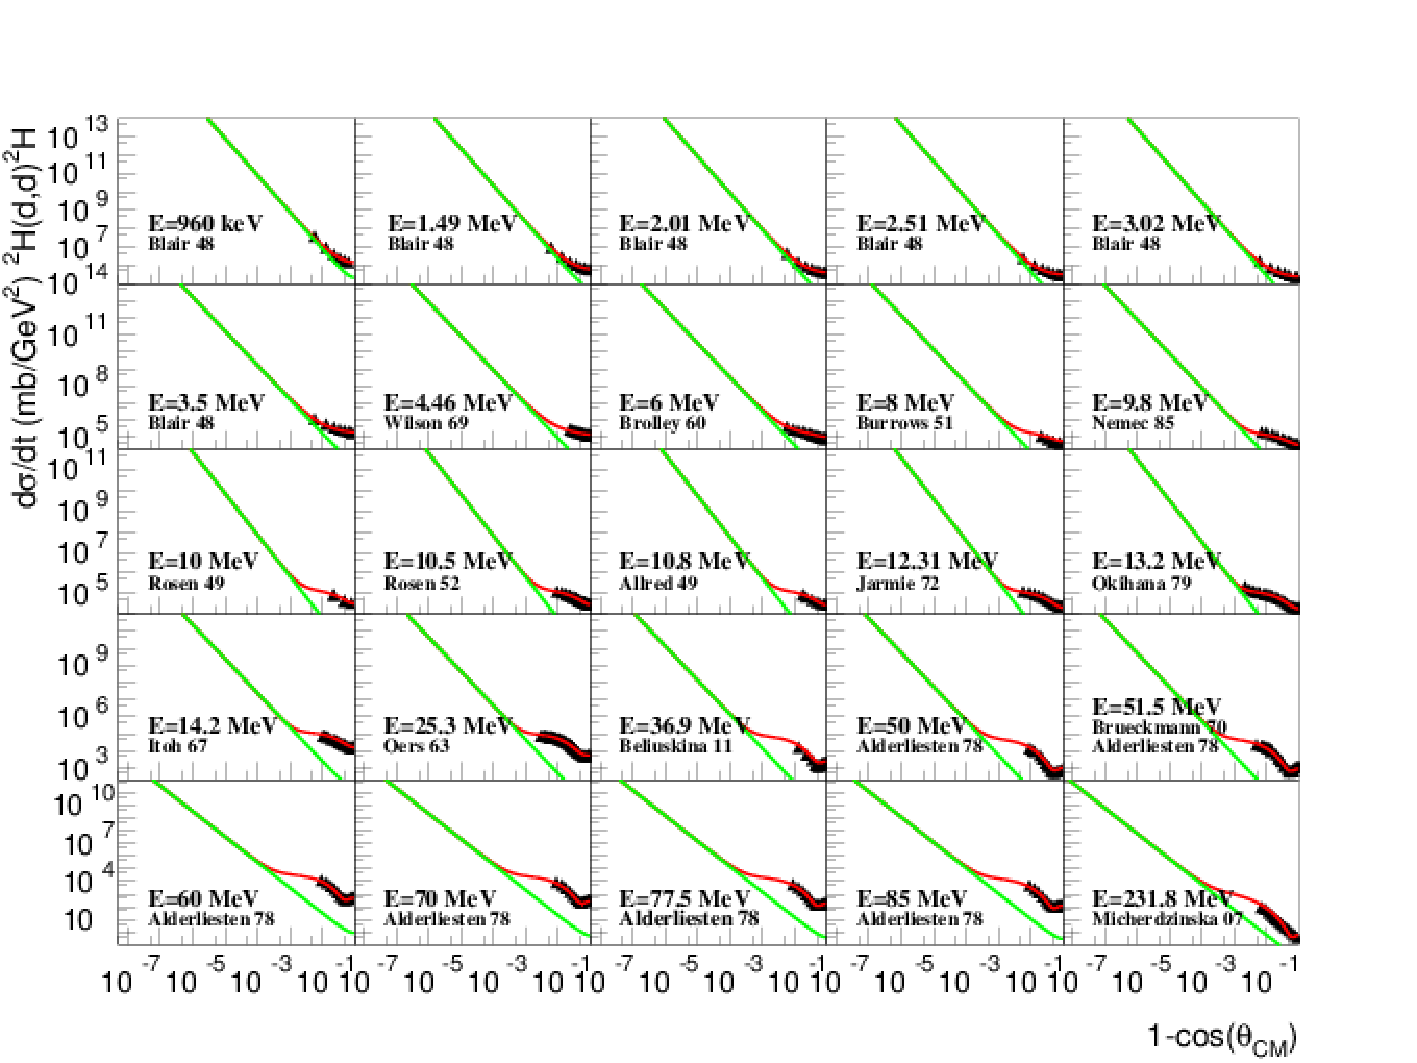
\includegraphics[width=0.99\linewidth]{images/difference_of_elastic_dd_from_rutherford_differential_cross_section.pdf}
  }
  \caption{Отличие дифференциального сечения рассеяния Резерфорда (зелёная кривая) от аппроксимации \cite{70/778-T} полного упругого дифференциального сечения D-D рассеяния (красная кривая) при различных кинетических энергиях налетающего дейтрона. Чёрными точками показаны использовавшиеся для аппроксимации экспериментальные данные, бравшиеся из базы ядерных данных EXFOR \cite{DD1_Blair,DD2_Wilson,DD3_Brolley,DD4_Burrows,DD5_Nemec,DD6_Rosen1,DD7_Rosen2,
  DD8_Allred,DD9_Jarmie,DD10_Okihana,DD11_Itoh,DD_Oers,DD12_Beliuskina,DD13_Alderliesten,
  DD14_Brueckmann,DD15_Micherdzinska}.}
  \label{fig:DifferenceOfElasticDDFromRutherfordDifferentialCrossSection}
\end{figure}	
	
	В разрабатываемом параллельном программном коде был написан процесс упругого D-D рассеяния, который возвращает сечение и конечное состояние (на вход подаётся налетающий дейтрон, на выходе получается 2 частицы: рассеянный дейтрон и дейтрон отдачи) данной неупругой реакции для налетающего дейтрона.
	Для проверки получающегося в ходе моделирования углового распределения в тонкую мишень из дейтерида титана запускались $N_P=100$ миллионов дейтронов с одной из 4 произвольно выбранных кинетических энергий налетающего дейтрона из Рис. ~\ref{fig:DifferenceOfElasticDDFromRutherfordDifferentialCrossSection}: 0.96 МэВ, 10 МэВ, 14.2 МэВ и 231.8 МэВ.
	Сечение неупругой реакции было искусственно поставлено равным максимальному значению переменной типа $double$ языка С++, равному $1.8 \cdot 10^{308}$, так что каждый из запущенных дейтронов участвовал в неупругой реакции в материале мишени, после чего исключался из моделирования, так как было необходимо только собрать гистограмму количества частиц $N_i$, попавших в интервалы лошарифмической шкалы по $1-\cos{\theta_{CM}}$, для того чтобы проверить получающееся на выходе моделирования дифференциальное сечение.
	В качестве оси абсцисс была выбрана величина $1-\cos{\theta_{CM}}$, а не $\cos{\theta_{CM}}$, т. к. выражающая квадрат переданного во взаимодействии импульса мандельстамовская переменная имеет вид $|t|=2\cdot p^2_{CM} \cdot \left( 1- \cos{\theta_{CM}} \right)$, а также потому что $1-\cos{\theta_{CM}}$ изменяется от 0 до 2 и с ней удобнее и нагляднее работать.
	Полученные количества событий в каждом бине $N_i$ делились на полное количество запущенных дейтронов $N_P$ и умножались на полную величину проинтегрированной аппроксимации упругого сечения (получена в \cite{70/778-T}) от $10^{-3} \cdot |t|_m$ до $|t|_m$.
	Таким образом, получались величины $\Delta \sigma_i$ в каждом бине.
	За верхний предел интегрирования бралась величина $|t|=2\cdot p^2_{CM}$, а не $|t|_{max}=4\cdot p^2_{CM}$, т. к. рассеивались тождественные частицы и поэтому максимальный угол рассеяния был $\theta_{CM}=\frac{\pi}{2}$.
	Почему за нижний предел интегрирования была выбрана величина $10^{-3} \cdot |t|_m$, будет объяснено ниже в разделе, описывающем реализацию процесса неупругого рассеяния в разрабатываемом программном коде.
	
	Шкала $1-\cos{\theta_{CM}}$ была логарифмической.
	Поэтому, чтобы извлечь величину дифференциального сечения $\frac{d\sigma}{d|t|}$ из полученной гистограммы, нужно было полученные значения $\Delta \sigma_i$ в каждом бине поделить на шаг по $|t|$ в каждом бине $\Delta |t|_i=|t|_{i+1}-|t|_i$, где $i$ изменялось от 0 до $N_{bin}-1$, $N_{bin}$ -- число бинов в гистограмме.
	
	После описанной процедуры моделирования гистограммы отношений величин $\frac{\Delta \sigma_i}{\Delta |t|}$, полученных в ходе моделирования, к точно вычисленным в среднегеометрической середине логарифмического бина по аппроксимации дифференциального сечения упругого D-D рассеяния, полученной в \cite{70/778-T}, значениям $\frac{d\sigma}{d|t|}$, для кинетических энергий налетающего дейтрона 0.96 МэВ, 10 МэВ, 14.2 МэВ и 231.8 МэВ, показаны на Рис. ~\ref{fig:CheckDDApproximationFillingBinsOfHistogram}.
	Как видно из Рис. ~\ref{fig:CheckDDApproximationFillingBinsOfHistogram}, в пределах погрешности отношение, как и должно быть, равно 1.
	Т. е. угловое распределение упругого D-D рассеяния в разрабатываемом программном коде моделируется должным образом.
	
\begin{figure}[ht]
  {
     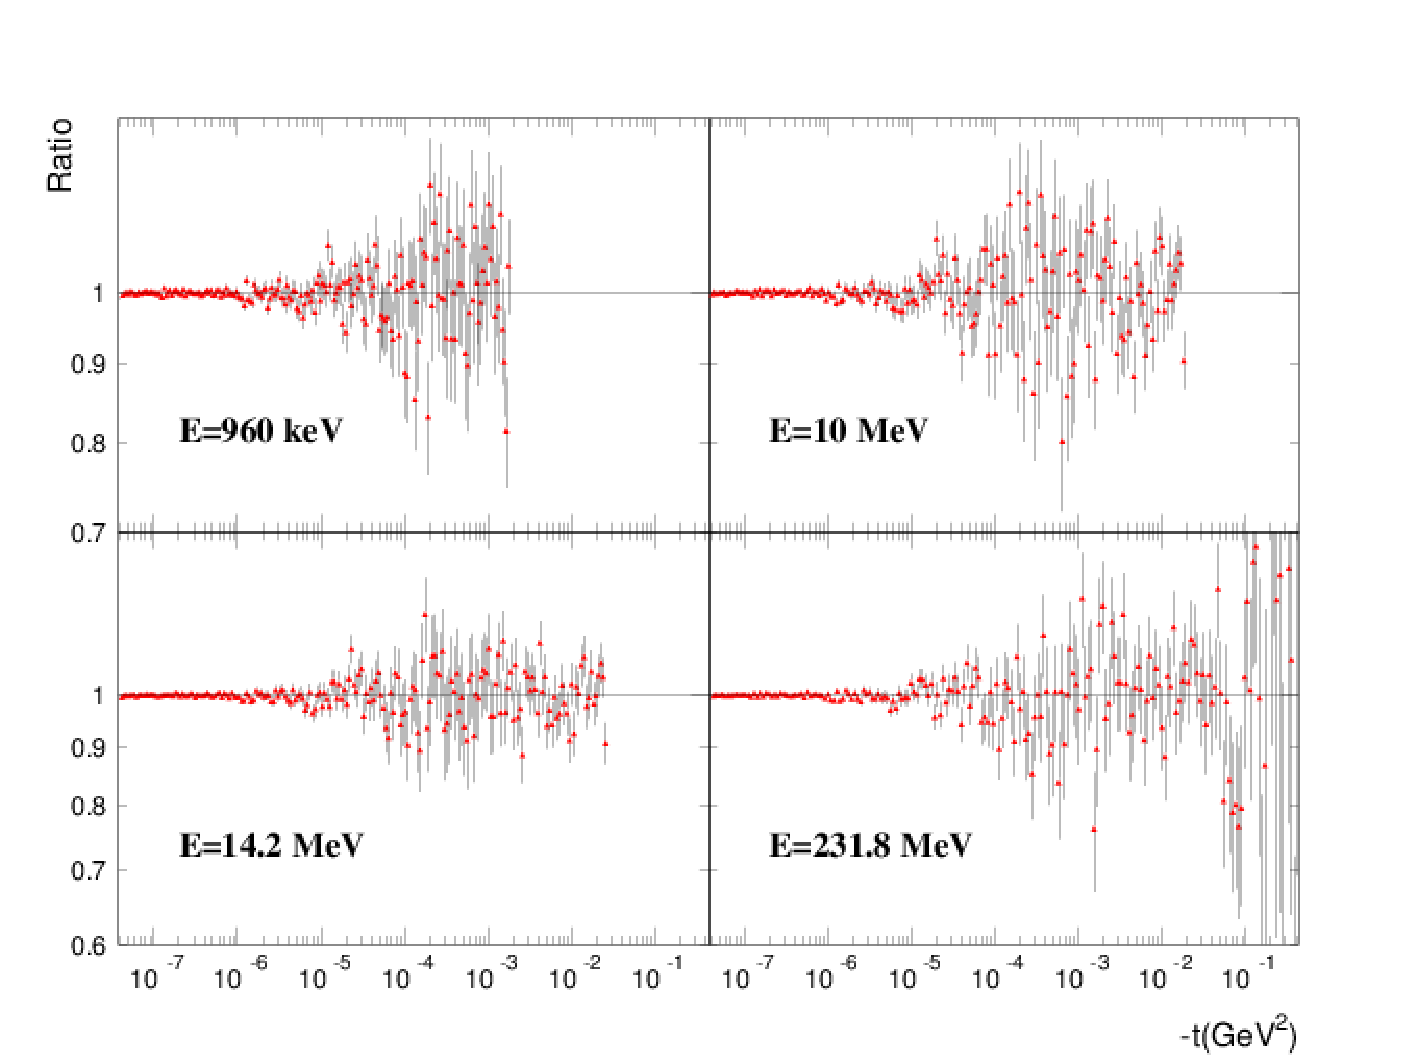
\includegraphics[width=0.99\linewidth]{images/check_dd_approximation_filling_bins_of_histogram.pdf}
  }
  \caption{Отношение дифференциального сечения упругого D-D рассеяния, полученного в ходе моделирования разрабатываемым параллельным программным кодом, к точной величине $\frac{d\sigma}{d|t|}$, вычисленной по аппроксимации дифференциального сечения упругого D-D рассеяния, полученной в \cite{70/778-T}, в среднегеометрических серединах логарифмических бинов гистограммы. Кинетические энергии налетающих дейтронов: 0.96 МэВ, 10 МэВ, 14.2 МэВ и 231.8 МэВ.}
  \label{fig:CheckDDApproximationFillingBinsOfHistogram}
\end{figure}


\clearpage{}
\section{Валидация энергетической зависимости линейных электронных потерь энергии $\frac{dE}{dx}$ ионов в дейтериде титана.}
\label{ValdEdx}
\subsection{Кривые энергетических потерь $\frac{dE}{dx}$ для ионов дейтерия и титана в дейтериде титана.}
\label{ValdEdx1}

	Средняя мера энергетических потерь заряженных частиц в веществе обозначается величиной $\frac{dE}{dx}$, равной усреднённым энергетическим потерям заряженной частицы с заданной кинетической энергией от всех взаимодействий и физических процессов, в которых она участвует, на единицы дины её пути в веществе.
	Обычно зависимость кривой энергетических потерь заряженных частиц в веществе $\frac{dE}{dx}$ от кинетической энергии налетающей частицы $T_{LS}$ задаётся формулой Бете-Блоха:
	
\begin{equation}
  \label{BetheBloch}
    \frac{dE}{dx}=\frac{Kz^2Z}{A\beta^2}\left[\frac{1}{2}ln\left(\frac{2m_ev^2\gamma^2T_{max}}{I^2}          \right)-\beta^2-\frac{\delta(\beta\gamma)}{2}\right],
\end{equation}
  	где $K=0.307075\frac{MeV\cdot cm^2}{mol}$, $z$ -- заряд налетающего иона, $Z$ -- заряд ядер вещества, $A$ -- атомный вес вещества, $m_e$ -- масса электрона, скорость налетающей частицы $v=c\beta$, величина $T_{max}$ определяет максимальную энергию, которую может передать налетающая частица свободному электрону при столкновении и $I$ -- средний потенциал ионизации, который обычно является подгоночным параметром при аппроксимации экспериментальных данных.
  	Коэффициент $\delta(\beta\gamma)$ отвечает за параметризацию эффекта плотности.
  
  	Как видно из формулы (\ref{BetheBloch}), если рассматриваются кривые $\frac{dE}{dx}$ для разных ионов в одном и том же веществе, то в первом приближении, если не учитывать отличие слагаемых в скобках, можно считать, что коэффициент отличия есть $\frac{z^2}{\beta^2}$.
  	Т. к. $c=1$, то $\beta^2=v^2 \sim \frac{T_{LS}}{m}$, где $m$ -- масса частицы, рассеивающейся в мишени.
  
  	Т. е. если, допустим, известна кривая энергетических потерь $\frac{dE}{dx}$ для ионов дейтерия в дейтериде титана, то по ней можно получить $\frac{dE}{dx}$ для титана в дейтериде титана используя скейлинговый коэффициент $\frac{z^2}{\beta^2}$.
 	В процессе моделирования ионного каскада  в мишени из дейтерида титана, инициированного облучением мишени интенсивным потоком дейтронов с кинетической энергией $T_{LS}=100$ кэВ, присутствуют 2 процесса, приводящие к появлению отличных от дейтронов частиц.
 	Это реакция неупругого рассеяния, имеющая 2 выходных канала: n + $^3_2He$ и p + t, и упругое ион-ионное рассеяние, в результате которого могут появиться либо дейтрон, либо ион титана.
 	Т. к. вероятность непругой реакции по отношению к упругому ион-ионному рассеянию при $T_{LS}=100$ кэВ, равняется $10^{-5}$ [откуда это взято????], то в первую очередь, конечно, нужно знать кривые энергетических потерь $\frac{dE}{dx}$ для ионов дейтерия и титана в дейтериде титана.
  
 	В базе данных для протонов PSTAR даны аппроксимации электронных потерь $\frac{dE}{dx}$ для протонов в дейтериде титана.
 	Из-за крайне малого времени релаксации не представляется возможным измерить зависимость $\frac{dE}{dx}$ для изотопов водорода в дейтериде титана.
 	Таких экспериментальных данных просто нет.
 	Также не удалось найти и данных по $\frac{dE}{dx}$ для ионов титана в дейтериде титана, их тоже не представляется возможным экспериментально измерить из-за тождественности налетающих частиц и частиц материала мишени.
  
 	Поэтому была взята аппроксимация $\frac{dE}{dx}$ для протонов в титане, показанная на Рис. ~\ref{fig:DeDxInTiD2Plot}.
 	Эти точки аппроксимации из базы данных PSTAR в свою очередь были проаппроксимированы нами в виде непрерывной функции:
  
\begin{equation}
  \label{dEdxHInTiD2Approximation}    
	  \frac{1}{z^2} \cdot \frac{dE}{dx}=\frac{1.007}{ \left( \frac{T_{LS}}{m} \right)^{0.74}+1.29 \cdot 10^{-5} \cdot \left( \frac{T_{LS}}{m} \right)^{-0.52} } + 6.74 \cdot \left[ F_4 \left( \frac{T_{LS}}{m} \right) \right]^{2.02},
\end{equation}

	где $F_n$ рекурсивно определяется следующим образом: $F_0=\ln{\left( 1+\frac{T_{LS}}{m} \right)}$, $F_1=\ln{\left( 1+F_0 \right)}$, $F_2=\ln{\left( 1+F_1 \right)}$ и т. д.
	Аппроксимирующая функция (\ref{dEdxHInTiD2Approximation}) изображена на Рис. ~\ref{fig:DeDxInTiD2Plot} розовой кривой. Аппроксимирующие $\frac{dE}{dx}$ кривые для дейтронов и ионов титана изображены на Рис. ~\ref{fig:DeDxInTiD2Plot} синим и красным цветом.
	Они были получены в результате скейлинга функции (\ref{dEdxHInTiD2Approximation}) по оси ординат на коэффициент $z^2$ квадрата заряда иона, для которого $\frac{dE}{dx}$ необходимо вычислить, и по оси абсцисс на коэффициент $\frac{m}{m_D}$, где $m_D$ -- масса дейтрона, равная 1875.6 МэВ, а $m$ -- масса иона, для которого необходимо рассчитать $\frac{dE}{dx}$. 
  
\begin{figure}[ht]
  {
     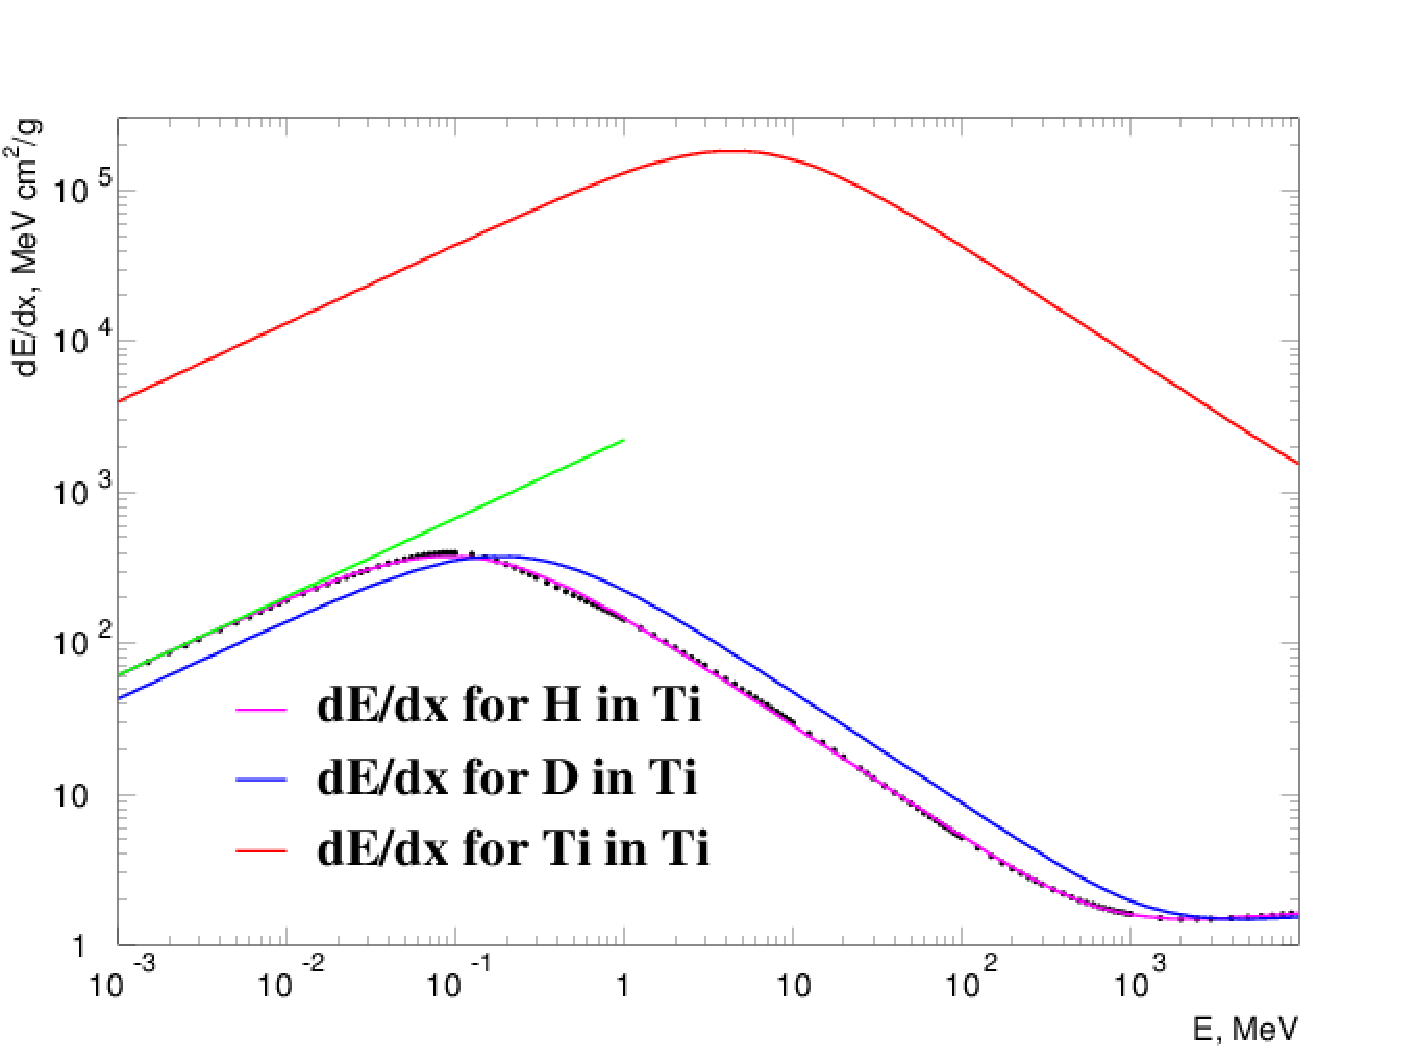
\includegraphics[width=0.99\linewidth]{images/dedx.pdf}
  }
  \caption{Кривые энергетических потерь $\frac{dE}{dx}$ для протонов, дейтронов и ионов титана в дейтериде титана. Чёрные точки -- аппроксимация $\frac{dE}{dx}$ для протонов в дейтериде титана, взятая из базы данных PSTAR для протонов. Розовая кривая $\frac{dE}{dx}$ для протонов -- выпоненная нами аппроксимация этих данных. Остальные -- синяя для дейтронов и красная для протонов -- кривые $\frac{dE}{dx}$ получены умножением розовой аппроксимационной кривой на скейлинговый фактор $\frac{z^2 \cdot m}{T_{LS}}$. Зелёная кривая показывает как $\frac{dE}{dx}$ экстраполируется к $T_{LS}=0$ МэВ, т. к. экспериментальной аппроксимации энергетических потерь в области малых энергий нет.}
  \label{fig:DeDxInTiD2Plot}
\end{figure}

	Зелёной кривой показана экстраполяция $\frac{dE}{dx}$ для протонов в дейтериде титана в область малых энергий.
	Известно, что по Линхарду эта экстраполяция должна быть $\sim \sqrt{v}$.
	Если в (\ref{dEdxHInTiD2Approximation}) сделать предельный переход $T_{LS} \to 0$, получается следующая функция экстраполяции $\frac{dE}{dx}$ в область малых $T_{LS}$:

\begin{equation}
  \label{dEdxLinhardExtrapolationInSmallTls}	
  \frac{dE}{dx}^{extra}=7.79 \cdot 10^4  \cdot z^2 \left( \frac{T_{LS}}{m} \right)^{0.52}.
\end{equation}

\subsection{Сравнение быстродействия вычисления $\frac{dE}{dx}$ по таблице и по функции.}
\label{ValdEdx2}	

	При моделировании в разрабатываемом параллельном программном коде линейных потерь энергии частиц в материале мишени есть 2 возможности: вычислять значение $\frac{dE}{dx}$ по таблице и по аппроксимирующей $\frac{dE}{dx}$ функции.
	
	Как видно из Рис. ~\ref{fig:DeDxInTiD2Plot}, у нас в распоряжении имеются чёрные точки аппроксимации электронной $\frac{dE}{dx}$ протонов в дейтериде титана, взятые из базы данных PSTAR.
	Они соответствуют таблице ($T_{LSi}$, $\frac{dE}{dx}_i$), где номер бина $i$ изменяется от 0 до 131, т. е. всего 132 пары величин ($T_{LS}$, $\frac{dE}{dx}$).
	При помощи описанного выше скейлинга из точек для протонов можно получить точки аппроксимации для дейтронов и ионов титана.
	Тогда по ним можно будет находить значение $\frac{dE}{dx}$ при заданной кинетической энергии $T_{LS}$ налетающей частицы следующим образом: сначала с помощью бинарного поиска находится бин $i$, куда частица попала по кинетической энергии $T_{LS}$.
	Далее, при помощи линейной интерполяции можно найти значение $\frac{dE}{dx}=\frac{dE}{dx}_i+\frac{ T_{LS}-T_{LSi} }{ T_{LSi+1}-T_{LSi} } \cdot \left( \frac{dE}{dx}_{i+1}-\frac{dE}{dx}_{i} \right)$.
	Если $T_{LS}$ было больше верхней границы $T_{LSi}$, т. к. данных аппроксимации нет, возвращался 0, если $T_{LS}$ был ниже нижней границы $T_{LSi}$, возвращалось значение $\frac{dE}{dx}$, вычисленное по функции (\ref{dEdxLinhardExtrapolationInSmallTls}) экстраполяции $\frac{dE}{dx}$ к нулю по $T_{LS}$.
	
	 Или же можно было использовать полученную функцию (\ref{dEdxHInTiD2Approximation}) аппроксимации $\frac{dE}{dx}$ ионов в дейтериде титана и точно по ней вычислять значение средних потерь энергии.
	 
	 Задача была проверить, какой из этих 2 способов вычисления $\frac{dE}{dx}$ работает быстрее при параллельном моделировании большого количества частиц.
	 Проверка проводилась для $\frac{dE}{dx}$ дейтронов в дейтериде титана, но очевидно, что точно такой же результат будет и для протонов, и для ионов титана в дейтериде титана.
	 В диапазоне $T_{LS}$ от $T^{min}_{LS}=200$ эВ до $T^{max}_{LS}=20$ МэВ с линейным шагом $\Delta T_{LS}=\frac{T^{max}_{LS}-T^{min}_{LS}}{N-1}$, где $N$ -- число вызовов функции, вычисляющей $\frac{dE}{dx}$, и при каждом вызове для очередного значения кинетической энергии вычислялось значение $\frac{dE}{dx}$.
	 Вычисления проводились параллельно и с использованием векторизации.
	 Сначала запускалась функция, вычислявшая $\frac{dE}{dx}$ по таблице, затем - по аппроксимирующей функции (\ref{dEdxHInTiD2Approximation}).
	 Замерялось время работы программы и делилось на число вызовов. Таким образом, получалось время 1 вызова функции, вычисляющей $\frac{dE}{dx}$, в зависимости от суммарного числа вызовов $N$.
	 И такие измерения были проведены в широком диапазоне по $N$ на различных вычилительных платформах, имеющихся во ВНИИА.
	 
	 Результат представлен на Рис. ~\ref{fig:CompareParallellydEdx}.
	 Как из него видно, самой производительной оказалась видеокарта Nvidia Titan V.
	 На ней при суммарных $10^{11}$ вызовах функции вычисления $\frac{dE}{dx}$ отношение времени вычисления $\frac{dE}{dx}$ по таблице и по функции выходит на константу, равную 10.
	 Процессор ПК Intel Core i7-3770 почти в 3.7 раз более производителен при вычислении $\frac{dE}{dx}$ по таблице, чем по функции, при $N \geq 10^8$.
	 64-ядерный процессор Intel Xeon Phi KNL при $N \geq 2\cdot 10^9$ в 3.1 раз быстрее работает при вычислении $\frac{dE}{dx}$ по таблице, чем по функции.
	 Самый быстрый 36-ядерный (2 процессора по 18 ядер, соединённые вместе) узел кластера VKPP достигает отличия в производительности при вычислении по таблице и по функции в 4.4 раза при $N$ порядка $10^{10}$.
	 Оказалось, что старая довольно слабая видеокарта Nvidia GTX GeForce 650 Ti, установленная в корпусе ПК с CPU Intel Core i7, на данной задаче показывает более высокую производительность (примерно в 1.2 раза быстрее), чем центральный процессор.
	 Окончательное сравнение быстродействия различных вычислительных платформ при параллельном счёте, использующем векторизацию, представлено в таблице ниже.
	 Т. к. наименьшей производительностью в данном тесте, как видно из Рис. ~\ref{fig:CompareParallellydEdx}, обладает CPU Intel Core i7, в данной таблице представлены отношения времени выполнения функции, возвращающей $\frac{dE}{dx}$, на CPU Core i7 к временам её выполнения на интересующих вычислительных платформах при максимальных $N$.
	 
	 \begin{tabular}{|c|c|c|}
	 \hline 
	 CPU/GPU & Таблица & Функция \\ 
	 \hline 
	 Geforce 650 Ti & 1.2 & 0.7 \\ 
	 \hline 
	 KNL & 5 & 6.1 \\ 
	 \hline 
	 36-ядерный узел VKPP & 7.4 & 6.3 \\ 
	 \hline 
	 Titan V & 180 & 68 \\ 
	 \hline 
	 \end{tabular} 
	 
	При уменьшении числа вызовов на всех вычислительных платформах за исключением KNL и 36-ядерного узла VKPP вычиcление $\frac{dE}{dx}$ по функции оказывается немного быстрее вычисления по таблице.
	Для KNL при уменьшении N они совпадают, а для 36-ядерного узла VKPP почему-то оказывается значительно быстрее вычисление по таблице.
	Вероятно, это связано в процессорной архитектурой, ведь на 36-ядерном узле VKPP 2 18-ядерных процессора соединены вместе.
	Также влияние может оказывать размер кэшей, вероятно, из-за большого количества ядер они там урезанные.
	
	То, что GPU Titan V позже всех вычислительных платформ выходит на константу времени вызова функции, говорит о том, что она обладает самым большим из всех представленных вычислительных платформ потенциалом для высоконагруженных параллельных вычислений и оказывается полностью загруженной лишь при числе вызовов, большем $2 \cdot 10^{11}$. 
	 
	Как видно из Рис. ~\ref{fig:CompareParallellydEdx}, при параллельном счёте и использовании векторизации однозначно быстрее оказывается вычислять $\frac{dE}{dx}$ по таблице, используя бинарный поиск и линейную интерполяцию, чем точно считать значение по аппроксимирующей функции.
	 

\begin{figure}[ht]
  {
     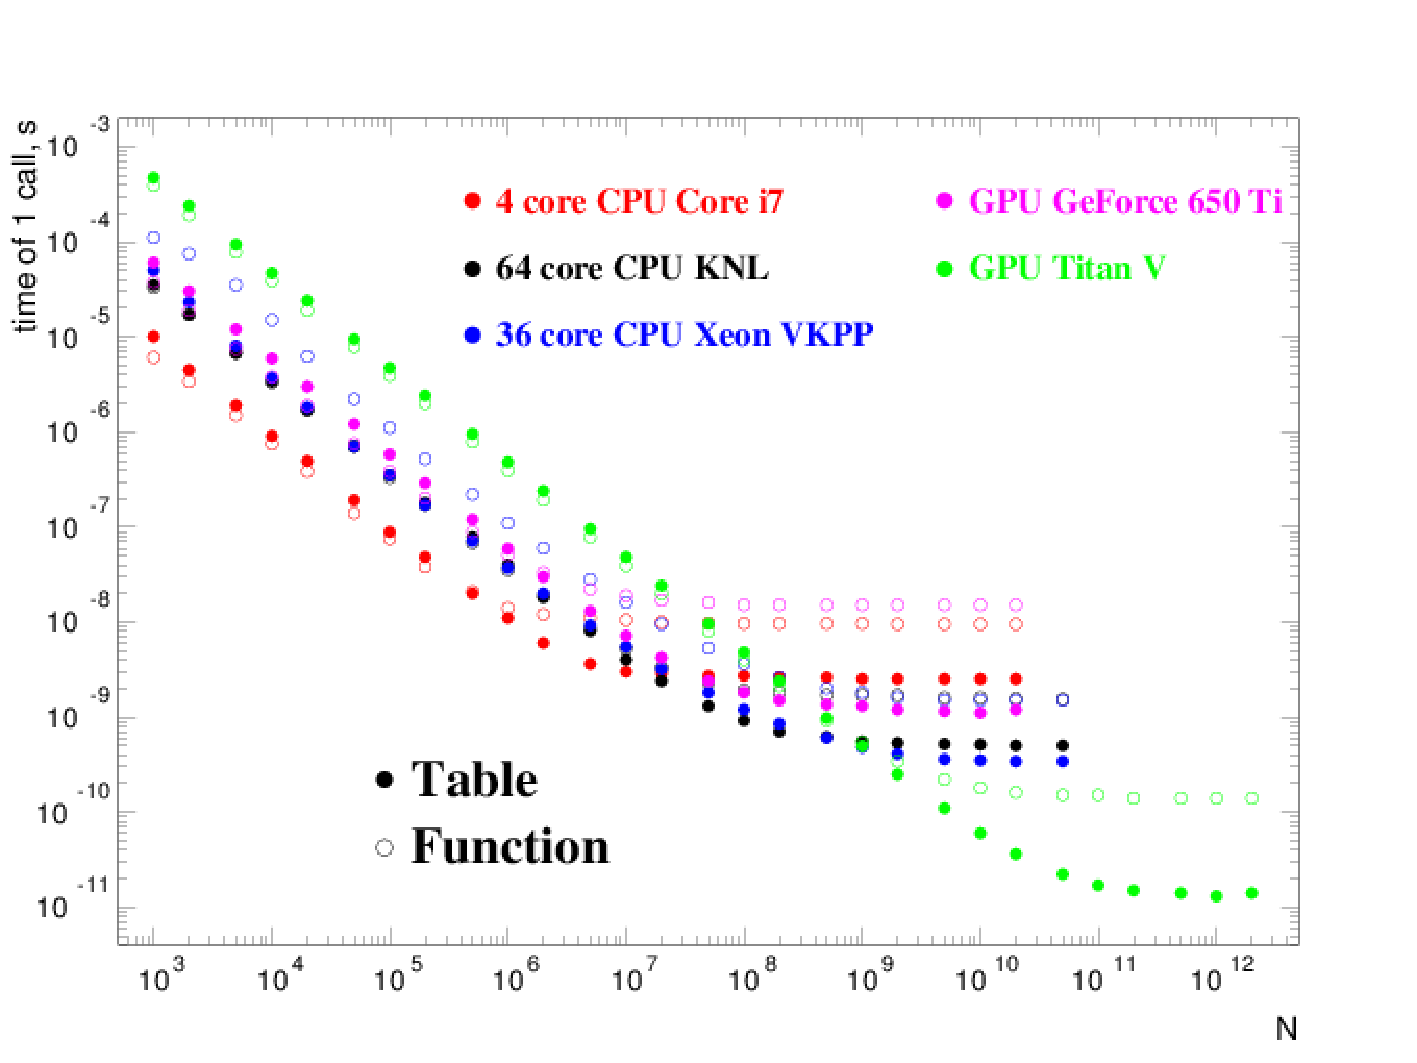
\includegraphics[width=0.99\linewidth]{images/compare_parallelly_dEdx.pdf}
  }
  \caption{Быстродействие программной функции вычисления $\frac{dE}{dx}$ по таблице (чёрные круги) и по аппроксимационной функции (\ref{dEdxHInTiD2Approximation}) (чёрные окружности) на различных вычислительных платформах, имеющихся во ВНИИА, в зависимости от числа вызовов программной функции в параллельном расчёте. Данный параллельный расчёт использует максимально возможное распараллеливание по потокам и векторизацию.}
  \label{fig:CompareParallellydEdx}
\end{figure}

	Также было интересно посмотреть, как изменится быстродействие и соотношение производительностей при однопоточном расчёте без использования векторизации.
	Данные измерения были произведены, и их результат представлен на Рис. ~\ref{fig:CompareSequentiallydEdx}.
	
\begin{figure}[ht]
  {
     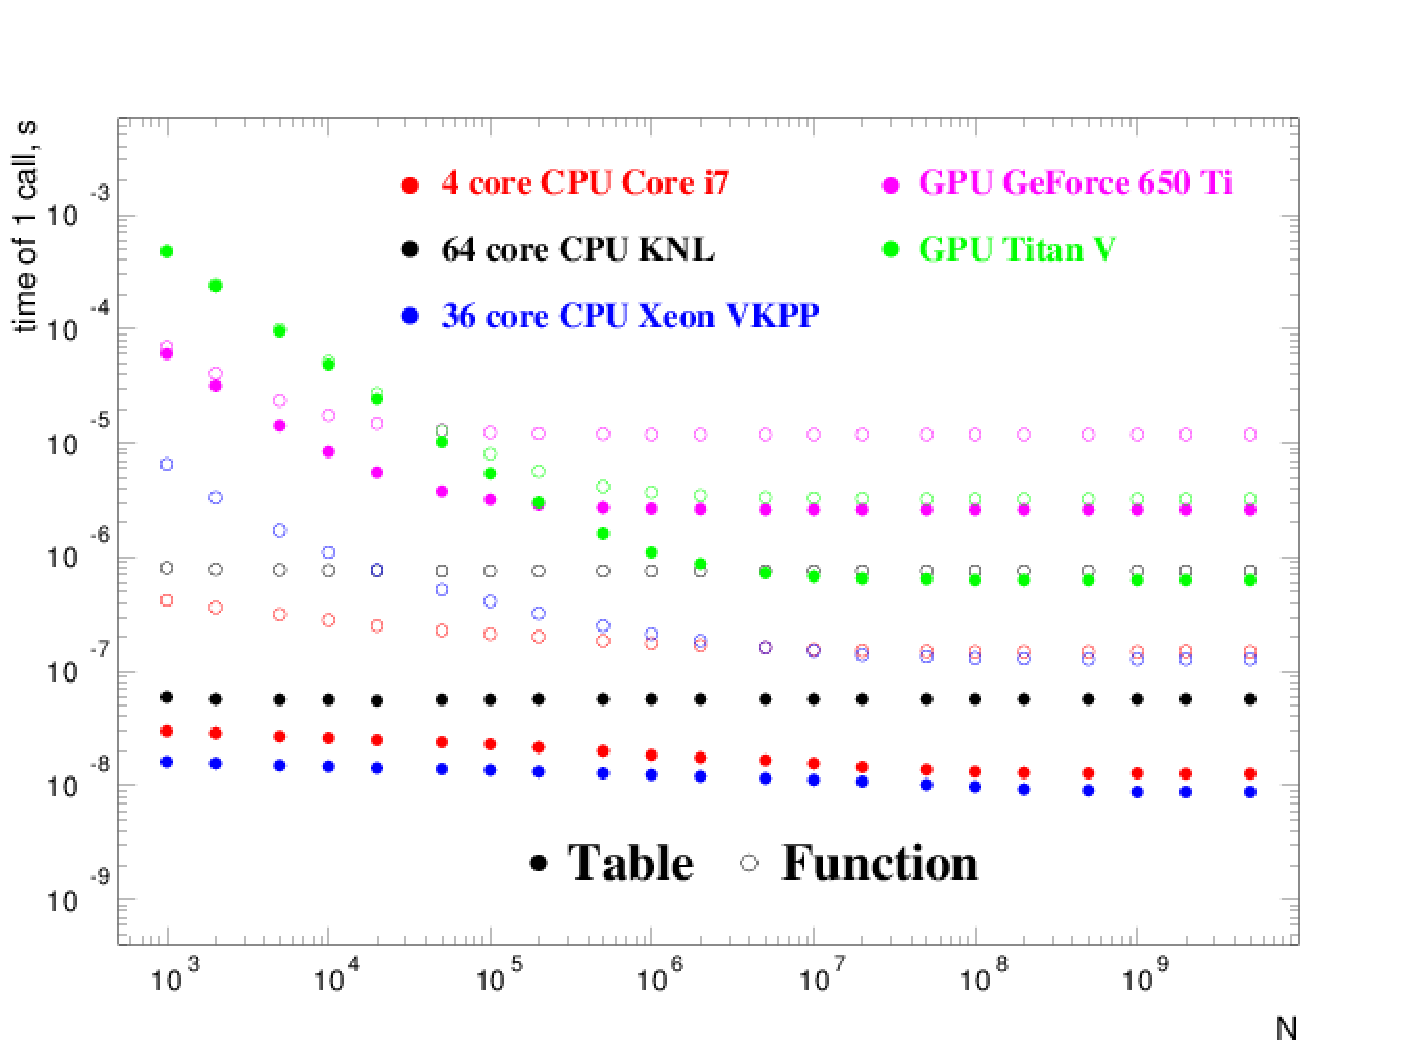
\includegraphics[width=0.99\linewidth]{images/compare_sequentially_dEdx.pdf}
  }
  \caption{Быстродействие программной функции вычисления $\frac{dE}{dx}$ по таблице (чёрные круги) и по аппроксимационной функции (\ref{dEdxHInTiD2Approximation}) (чёрные окружности) на различных вычислительных платформах, имеющихся во ВНИИА, в зависимости от чила вызовов программной функции в однопоточном расчёте без использования векторизации.}
  \label{fig:CompareSequentiallydEdx}
\end{figure}

	За исключением GPU, 36-ядерного узла кластера VKPP и процессора Intel Core i7, все остальные платформы показывают почти константное время счёта при любом $N$.
	На GPU при уменьшении $N$ наблюдается увеличение времени вызова при вычислении $\frac{dE}{dx}$ и по таблице, и по функции.
	Вероятно, этот эффект связан с особенностями архитектуры GPU. Почему-то он наблюдается и при вычислении $\frac{dE}{dx}$ по аппроксимирующей функции на 36-ядерном узле кластера VKPP. 
	
	При запуске последовательного и невекторизованного кода самую слабую производительность показала GPU GeForce 650 Ti.
	Поэтому ниже приведена таблица, в которой представлены отношения времени вызова функции, вычисляющей $\frac{dE}{dx}$, на GPU GeForce 650 Ti, к времени её вызова на интересующей вычислительной платформе при максимальных $N$.

	 \begin{tabular}{|c|c|c|}
	 \hline 
	 CPU/GPU & Таблица & Функция \\ 
	 \hline 
	 Titan V & 4.1 & 3.7 \\ 
	 \hline 
	 KNL & 45 & 16 \\ 
	 \hline 
	 Core i7 & 206 & 80.1 \\ 
	 \hline 
	 36-ядерный узел VKPP & 298 & 93 \\ 
	 \hline 
	 \end{tabular} 

	Т. е. при запуске последовательного кода без векторизации самыми быстрыми оказались центральный процессор ПК Intel Core i7-3770 и процессор Intel Xeon E5-2697 36-ядерного узла кластера VKPP и самыми медленными видеокарты.
	Это понятно: у этих CPU самые большие тактовые частоты (базовые частоты у E5 – 2.3 ГГц, у Core i7 – 3.4 ), а у GPU самые медленные (у GPU GeForce 650 Ti -- 1.1ГГц, у Titan V -- 1.5 ГГц).
	Т. к. код исполняется последовательно, то фактически его быстродействие определяется тактовой частотой процессора, на котором он исполняется.
	
	Из только что проведённого исследования производительности вычисления значения $
\frac{dE}{dx}$ по таблице при помощи бинарного поиска и линейной интерполяции и по аппроксимирующей функции однозначно следует, что при высоконагруженных параллельных расчётах значительно быстрее работает вычисление $\frac{dE}{dx}$ по таблице, чем по функции.
	Поэтому в разрабатываемом параллельном программном коде все операции вычисления $\frac{dE}{dx}$ выполнялись с помощью бинарного поиска и линейной интерполяции по таблице аппроксимации линейных электронных потерь энергии, взятой из базы данных PSTAR для протонов и преобразованной для дейтронов и ионов титана с помощью описанного скейлинга.
	Если же величина кинетической энергии дейтрона была меньше минимального значения $T_{LS}$ в полученной с помощью скейлинга базе данных, то значение $\frac{dE}{dx}$ вычислялось при помощи эктраполяции (\ref{dEdxLinhardExtrapolationInSmallTls}) в область малых $T_{LS}$.

  
  

\clearpage{}
\section{Программная реализация процессов физических взаимодействий.}
\subsection{Описание типового дискретного процесса рассеяния частицы в среде.}
\label{TypicalPhysicalProcessDescription}

	Реализация всех процессов упругого ион-ионного и D-D рассеяния, неупругой D-D реакции, а в будущем и других физических процессов, делалась единообразным образом.
	
	На вход программе подавался вектор 4-импульса $\vec{p}\,^{inc}_{LS}$=($p_x$, $p_y$, $p_z$, $E^{inc}_{LS}$) рассеивающейся или участвующей в реакции частицы и её PDG-код \cite{PDG}, определяющий вид частицы.
	Импульс налетающей частицы $\vec{p}\,_{LS}^{inc}$ =($p_x$,$p_y$,$p_z$,$E^{inc}_{LS}$) переводился из лабораторной системы в систему центра масс следующим образом.
	Т. к. в лабораторной системе ядро мишени -- при моделировании ионного каскада в мишени из дейтерида титана это расположенное в узле кристаллической решётки ядро дейтерия либо титана -- покоилось, то из соотношений Лоренца следовало, что
\begin{equation}
\label{PLStoCM}
\begin{aligned} 
  \vec{p}_{CM} = \gamma \left( \vec{p}\,_{LS}^{inc} - \vec{V}_{CM} \cdot E_{LS}^{inc} \right) = \vec{p}\,_{LS}^{inc} \cdot \frac{M}{\sqrt{s}},
\end{aligned}
\end{equation}
где гамма-фактор равен $\gamma=\frac{E_{LS}^{inc}+M}{\sqrt{s}}$, $\vec{V}_{CM} = \frac{\vec{p}\,_{LS}^{inc}}{E_{LS}^{inc}+M}$ -- скорость системы центра масс, мандельстамовская переменная $s$ определяется выражением

\begin{equation}
  \label{MandelStahmSVariableDefinition}    
  s=m^2+2 \cdot E^{inc}_{LS} \cdot M + M^2,
\end{equation}
	а $m$ и $M$ -- массы налетающей частицы и ядра отдачи соответственно, вычисляемые по их PDG-коду. 

	Таким образом, по импульсу $\vec{p}\,_{LS}^{inc}$ и энергии $E_{LS}^{inc}$ налетающей частицы в лабораторной системе получались импульс в системе центра масс $\vec{p}_{CM}$ и энергия налетающей частицы в системе центра масс $E^{inc}_{CM}=\sqrt{m^2+p_{CM}^2}$.
	
	Далее, необходимо было разыграть с помощью случайного числа и извлечь из соответствующей типу взаимодействия специально подготовленной базы данных значение косинуса угла рассеяния в системе центра масс $\cos{\theta_{CM}}$.
	
	После того как угол рассеяния в системе центра масс $\theta_{CM}$ был посчитан, импульс в системе центра масс после рассеяния определялся как
\begin{equation}
\label{CMMomentumFin}
\begin{aligned} 
  {\vec{p}}\,_{CM}^{fin} = p_{CM}\cdot\left(\cos{\theta_{CM}} \cdot \vec{e}_1 + \sin{\phi} \cdot   \sin{\theta_{CM}} \cdot \vec{e}_2 +  \cos{\phi} \cdot \sin{\theta_{CM}} \cdot \vec{e}_3\right),
\end{aligned}
\end{equation}
где $\vec{e}_1$ -- единичный вектор в направлении $\vec{p}_{CM}$, $\vec{e}_2$ и $\vec{e}_3$ -- произвольные взаимно перпендикулярные единичные вектора, перпендикулярные $\vec{e}_1$, а $\phi$ -- случайный угол от $0$ до $2\pi$.
	
	В случае упругого рассеяния $\vec{p}_{CM}$ в результате взаимодействия не меняется по модулю, лишь по направлению.
	Но при реакции неупругого D-D рассеяния, т. к. взаимодействие неупругое, $p_{CM}$ изменяется.
	И это также необходимо учитывать. 
	
	После осуществления взаимодействия в системе центра масс необходимо было перевести $\vec{p}\,^{fin}_{CM}$ обратно в лабораторную систему координат.
	Т. к. при преобразовании Лоренца изменяется только продольная (имеющая направление вдоль $\vec{V}_{CM}$) компонента вектора импульса, поперечная же остаётся неизменной, то необходимо было найти компоненту конечного вектора импульса в системе центра масс $\vec{p}\,^{fin}_{CM}$ вдоль $\vec{V}_{CM}$, а значит, вдоль $\vec{p}_{CM}$, т. к. ядро мишени покоится.
	Эта компонента, очевидно, равна $\vec{p}\,^{fin \parallel \vec{V}_{CM}}_{CM}=\vec{p}\,^{fin}_{CM} \cdot \frac{\vec{p}_{CM}}{p_{CM}}$.
	Компонента, перпендикулярная $\vec{p}_{CM}$, есть $\vec{p}\,^{fin \bot \vec{V}_{CM}}_{CM}=\vec{p}\,^{fin}_{CM}-\vec{p}\,^{fin \parallel \vec{V}_{CM}}_{CM}$.
	Для перевода $\vec{p}\,^{fin \parallel \vec{V}_{CM}}_{CM}$ из системы центра масс обратно в лабораторную систему использовалось преобразование Лоренца:
	
\begin{equation}
\label{MSlsincMomentumAfter}
\begin{aligned} 
  \vec{p}\,_{LS}^{fin \parallel \vec{V}_{CM}} = \gamma \left( \vec{p}\,^{fin \parallel \vec{V}_{CM}}_{CM} + \vec{V}_{CM} \cdot E^{fin}_{CM} \right),
\end{aligned}
\end{equation}
	где энергия рассеивающейся частицы в системе центра масс после рассеяния есть $E^{fin}_{CM}=\sqrt{m^2+\left( p^{fin}_{CM} \right)^2}$.
	
	Конечный импульс налетающей частицы находился исходя из того, что $\vec{p}\,^{fin \bot \vec{V}_{CM}}_{CM}$ не менялся при переходе между системами координат, и был равен:
	
\begin{equation}
\label{LSincMomentumAfter}
\begin{aligned} 
  \vec{p}\,_{LS}^{fin} = \vec{p}\,_{LS}^{fin \parallel \vec{V}_{CM}} + \vec{p}\,^{fin \bot \vec{V}_{CM}}_{CM}.
\end{aligned}
\end{equation}	
	
	Конечный импульс ядра мишени в лабораторной системе находился из закона сохранения импульса:
\begin{equation}
\label{LStargetMomentumAfter}
\begin{aligned} 
  \vec{p}\,_{LS}^{fin\,target} = \vec{p}\,_{LS}^{inc} - \vec{p}\,_{LS}^{fin}.
\end{aligned}
\end{equation}
	Полные энергии частиц изменялись как $E_{LS}^{fin\,inc}=\sqrt{m^2+\left( p_{LS}^{fin} \right)^2 }$ и $E_{LS}^{fin\,target}=\sqrt{M^2+\left( p_{LS}^{fin\,target} \right)^2 }$.
  
	Таков схематически единообразный алгоритм написания физических процессов упругой и неупругой ядерной реакции.
	По большому счёту, единственным отличием являются различные угловые распределения дифференциальных сечений физических процессов и изменение $p_{CM}$ в ходе неупругих взаимодействий.
	
\subsection{Реализация дискретного процесса неупругой D-D реакции.}
\label{InelasticDDReactionRealization}

	Интегральные сечения неупругой D-D реакции определяются выражениями (\ref{InelasticDDNHe3ChannelIntegralCrossSection}) и (\ref{InelasticDDPTChannelIntegralCrossSection}), дающими значение интегрального сечения одного из 2 каналов неупругой D-D реакции в барнах при данной кинетической энергии в системе центра масс $T_{CM}=\frac{T_{LS}}{2}$.
	
	Полное сечение реакции неупругого рассеяния определяется как сумма интегральных сечений обоих каналов неупругой D-D реакции при данной кинетической энергии налетающего дейтрона $T_{LS}$, умноженная на коэффициент $\frac{2}{3}$, равный количественной доле атомов дейтерия в молекуле $TiD_2$.
	
	При розыгрыше 4-импульсов налетающей частицы и ядра мишени при неупругой D-D реакции угловые зависимости дифференциального сечения неупругой D-D реакции определяются с помощью базы данных TPT, куда в свою очередь они были записаны в виде нормированных частичных сумм интегралов от полиномов Лежандра, коэффициенты которых приведены в базе данных ENDF-6.
	Например, при $T_{LS}=2$ МэВ нормированное дифференциальное сечение выглядит как показано на Рис. ~\ref{fig:ValidationThermonuclear2mev2billionParticles}.
	
	Т. к. реакция неупругая, импульс в системе центра масс $p_{CM}$ после взаимодействия изменяется как  \cite[стр.~321]{PDG}
	
\begin{equation}
\label{PCMInelasticDDAfterNHe3}
\begin{aligned} 
  p\,_{CM}^{fin} = \frac{ \sqrt{ \left( s-\left( m_n + m_{^3_2He}\right)^2 \right) \cdot \left( s-\left( m_n - m_{^3_2He} \right)^2 \right) } }{2\cdot \sqrt{s}}
\end{aligned}
\end{equation}

	для выходного канала n+$^3_2$He неупругой реакции D-D и как

\begin{equation}
\label{PCMInelasticDDAfterPT}
\begin{aligned} 
  p\,_{CM}^{fin} = \frac{ \sqrt{ \left( s-\left( m_p + m_t\right)^2 \right) \cdot \left( s-\left( m_p - m_t \right)^2 \right) } }{2\cdot \sqrt{s}}
\end{aligned}
\end{equation}

	для её выходного канала p+t.
	Здесь мандельстамовская переменная $s$ определяется выражением (\ref{MandelStahmSVariableDefinition}), а $m_n$, $m_p$, $m_t$ и $m_{^3_2He}$ -- массы нейтрона, протона, тритона и ядра $^3_2He$ соответственно.
	
	Соответственно, если на входе данному процессу должен подаваться налетающий дейтрон, то на выходе будут 2 частицы: либо n+$^3_2He$, либо p+t.
	
	Значение косинуса угла рассеяния в системе центра масс $\cos{\theta_{CM}}$ получалось с помощью бинарного поиска нужных элементов базы данных по кинетической энергии налетающего дейтрона в лабораторной системе $T_{LS}$, равномерно распределённого случайного числа $R$ от 0 до 1, бинарного поиска соответствующего $R$ значения $\cos{\theta_{CM}}$ в элементе базы данных нормированных частичных сумм, соответствующих различным значениям $\cos{\theta_{CM}}$ от -1 до 1, и квадратичной интерполяции значения $\cos{\theta_{CM}}$. 
	

\subsection{Реализация дискретного процесса упругого ион-ионного рассеяния.}
\label{ElasticIonIonScatteringRealization}

	
	В кристаллической решётке дейтерида титана энергия, необходимая для выбивания ионов титана и дейтерия из их равновесного положения в узлах решётки (так называемая ``displacement energy'') $E_{de}$, равняется примерно 25 эВ для титана и примерно 10 эВ для дейтерия.
  	Эти значения используются, например, в программе SRIM \cite{SRIM}, применяющейся для моделирования ионного транспорта, и программах молекулярной динамики.
  	Так как при кинетической энергии налетающей частицы, меньшей указанных значений, не происходит выбивания иона дейтерия либо титана из их равновесного положения в узле кристаллической решётки в результате Резерфордовского рассеяния, можно в качестве дифференциального сечения $\frac{d\sigma_{ms}}{d|t|}$ многократного рассеяния рассматривать дифференциальное сечение Резерфордовского рассеяния при $|t|$ от 0 до
\begin{equation}
\begin{aligned} 
 \label{Tmin}  
    |t|_{min}=2E_{de}M,
\end{aligned}
\end{equation}
	где $M$ -- масса ядра мишени, а значение $E_{de}$ берётся либо для дейтерия, либо для титана, в зависимости от того, на каком ядре рассеивается налетающая частица.
	Это и было сделано в отчёте \cite{70/778-T}.
	Там интегральное сечение многократного рассеяния представлялось в виде $\int \limits_0^{|t|_{min}} \frac{d\sigma_R}{d|t|} \cdot d|t|$, где $\frac{d\sigma_R}{d|t|}$ -- дифференицальное сечение Резерфордовского рассеяния.
	В результате моделирования, основывающегося на применении только что описанного интегрального сечения многократного рассеяния, была получена аппроксимация функции плотности вероятности углового распределения многократного рассеяния (\ref{MSApproximationFunction}) для дейтронов с кинетической энергией 10 МэВ в мишени из дейтерида титана.
	При помощи скейлинга, описанного в разделе \ref{subValMS2}, производился пересчёт полученного углового распределения функции плотности вероятности для произвольной кинетической энергии налетающего дейтрона и для произвольной кинетической энергии налетающего иона титана.
	
	Таким образом, при $0 \leq |t| \leq |t|_{min}$ рассматривается непрерывный процесс многократного рассеяния согласно аппроксимации (\ref{MSApproximationFunction}) и описанному в разделе \ref{subValMS2} скейлингу.
	При должном качестве аппроксимирующей функции (\ref{MSApproximationFunction}) и правильном методе скейлинга этот подход должен приводить к серьёзному ускорению моделирования без ухудшения качества его результатов.
	Ведь если отказаться от аппроксимирующей угловое распределение многократного рассеяния функции (\ref{MSApproximationFunction}), тогда многократное рассеяние будет входить в дискретное сечение процесса Резерфордовского рассеяния в качестве самой левой области интегрирования при самых малых углах рассеяния, ведь многократное рассеяние по сути есть многократное Резерфордовское рассеяние на малые углы.
	Но т. к. дифференциальное сечение Резерфордовского рассеяния в области $|t|=0$ огромно (интеграл $\sigma_R=\int \limits_0^{|t|_{max}} \frac{d\sigma_R}{d|t|} \cdot d|t|$, где $|t|_{max}=4\cdot p^2_{CM}$, сходится только лишь если учитывать электронную экранировку, делающую значение $\frac{d\sigma_R}{d|t|}$ конечным при $|t|=0$), это приведёт к тому, что средняя длина свободного пробега $\lambda=\frac{1}{n_{TiD_2} \cdot \sigma_R}$ будет наименьшей из средних длин свободного пробега для всех процессов, а это будет означать, что этот процесс будет всё время выигрывать, и частицы всё время будут сдвигаться на мизерный шаг, что в свою очередь приведёт к замедлению моделирования.
	
	Таким образом, при $0 \leq |t|_{min} \leq|t|_{max}$ рассматривается аппроксимация функции плотности вероятности углового распределения многократного рассеяния (\ref{MSApproximationFunction}), а при $|t| \geq |t|_{min}$ -- упругое рассеяние (для всех случаев рассеяния, кроме p-p, D-D, p-D и D-t, если не оговорено иное, рассматривается Резерфордовское рассеяние, т. к. сильным взаимодействием (сильной амплитудой рассеяния) можно пренебречь из-за кулоновского барьера).
	
	Дифференциальные сечения Резерфордовского рассеяния задаются следующими выражениями:
	
\begin{equation}
\label{DifferentialRutherfordCSDifferentParticles}
\begin{aligned} 
  \frac{d \sigma_R}{d|t|} = \frac{\pi}{p^2_{CM}} \cdot \left( \frac{ 2 \mu \alpha \hbar c z Z}{|t|} \right)^2 
\end{aligned}
\end{equation}

	для рассеяния различных частиц \cite{LandauLifshitzMechanics} и
	
\begin{equation}
\label{DifferentialRutherfordCSEqualParticles}
\begin{aligned} 
  \frac{d \sigma_R}{d|t|} = \frac{\pi}{p^2_{CM}} \cdot \left( 2 \mu \alpha \hbar c z Z \right)^2 \cdot               \Biggl( \frac{1}{|t|^2} + \frac{1}{\left( |t|_{max} - |t| \right)^2} + \\
  SIGN \cdot \frac{2}{2 \cdot S+1} \cdot
  \frac{1}{|t| \cdot \left( |t|_{max} -|t| \right)}
  \cdot \cos{ \left( \frac{\alpha}{\beta^r_{CM}}
  \cdot \ln{ \frac{|t|}{|t|_{max} -|t|} } \right)}
\Biggr)
\end{aligned}
\end{equation}

	для рассеяния тождественных частиц \cite{LandauLifshitzNonrelativisticQM}.
	Здесь $\mu=\frac{m\cdot M}{m+M}$ -- приведённая масса, $m$, $M$, $z$ и $Z$ -- массы и заряды налетающей частицы и мишени соответственно, $\alpha$ -- постоянная тонкой структуры, $\hbar c=200$ Мэв$\cdot$фм, $\beta^r_{CM}=\frac{1}{\sqrt{1+\left( \frac{\mu}{p_{CM}} \right)^2 }}$ -- скорость приведённой частицы в системе центра масс, $S$ -- спин частицы, а $SIGN$ определяется следующим образом: если спин частицы целый, то $SIGN=1$, если полуцелый, то $SIGN=-1$.
	
	Для случая D-D рассеяния выражение (\ref{DifferentialRutherfordCSEqualParticles}) принимает вид:
	
\begin{equation}
\label{DifferentialRutherfordCSEqualDD}
\begin{aligned} 
  \frac{d \sigma_R}{d|t|} = \frac{\pi}{p^2_{CM}} \cdot \left( m_D \alpha \hbar c \right)^2 \cdot               \Biggl( \frac{1}{|t|^2} + \frac{1}{\left( |t|_{max} - |t| \right)^2} + \\
  \frac{2}{3} \cdot
  \frac{1}{|t| \cdot \left( |t|_{max} -|t| \right)}
  \cdot \cos{ \left( \frac{\alpha}{\beta^r_{CM}}
  \cdot \ln{ \frac{|t|}{|t|_{max} -|t|} } \right)}
\Biggr).
\end{aligned}
\end{equation}

	Интегральное сечение (интеграл $\int \limits_{|t|_{min}}^{|t|_{max}} \frac{d\sigma_R}{d|t|} \cdot d|t|$ для различных частиц и интеграл $\int \limits_{|t|_{min}}^{|t|_{max}-|t|_{min}} \frac{d\sigma_R}{d|t|} \cdot d|t|$ для тождественных частиц) для различных частиц есть

\begin{equation}
\label{IntegralRutherfordCSDifferentParticles}
\begin{aligned} 
  \sigma_R = \frac{\pi}{p^2_{CM}} \cdot \left( 2 \mu \alpha \hbar c z Z \right)^2 \cdot \left( \frac{1}{|t|_{min}} - \frac{1}{|t|_{max}} \right) 
\end{aligned}
\end{equation}

	и для тождественных частиц:
	
\begin{equation}
\label{IntegralRutherfordCSEqualParticles}
\begin{aligned} 
  \sigma_R = 2 \cdot \frac{\pi}{p^2_{CM}} \cdot \left( 2 \mu \alpha \hbar c z Z \right)^2 \cdot               \Biggl( \frac{1}{|t|_{min}} - \frac{1}{|t|_{max} - |t|_{min}} + \\
  2 \cdot SIGN \cdot \frac{2}{2 \cdot S+1} \cdot
  \frac{1}{|t|_{max}} \cdot \frac{\beta^r_{CM}}{\alpha}
  \cdot \sin{ \left( \frac{\alpha}{\beta^r_{CM}}
  \cdot \ln{ \frac{|t|_{max} - |t|_{min}}{|t|_{min}} } \right)}.
\Biggr)
\end{aligned}
\end{equation}

	В случае D-D Резерфордовсокго рассеяния выражение (\ref{IntegralRutherfordCSEqualParticles}) принимает вид:
	
\begin{equation}
\label{IntegralRutherfordCSEqualDD}
\begin{aligned} 
  \sigma_R = 2 \cdot \frac{\pi}{p^2_{CM}} \cdot \left( m_D \alpha \hbar c\right)^2 \cdot               \Biggl( \frac{1}{|t|_{min}} - \frac{1}{|t|_{max} - |t|_{min}} + \\
  \frac{4}{3} \cdot
  \frac{1}{|t|_{max}} \cdot \frac{\beta^r_{CM}}{\alpha}
  \cdot \sin{ \left( \frac{\alpha}{\beta^r_{CM}}
  \cdot \ln{ \frac{|t|_{max} - |t|_{min}}{|t|_{min}} } \right)}
\Biggr).
\end{aligned}
\end{equation}

	Полученные в соответствии с только что написанными выражениями зависимости интегрального сечения от кинетической энергии в системе центра масс $T_{CM}=\frac{p^2_{CM}}{2\cdot \mu}$, показаны на Рис. ~\ref{fig:IntegralRutherfordDTiCrossSections} в дважды логарифмическом масштабе.

\begin{figure}[ht]
  {
     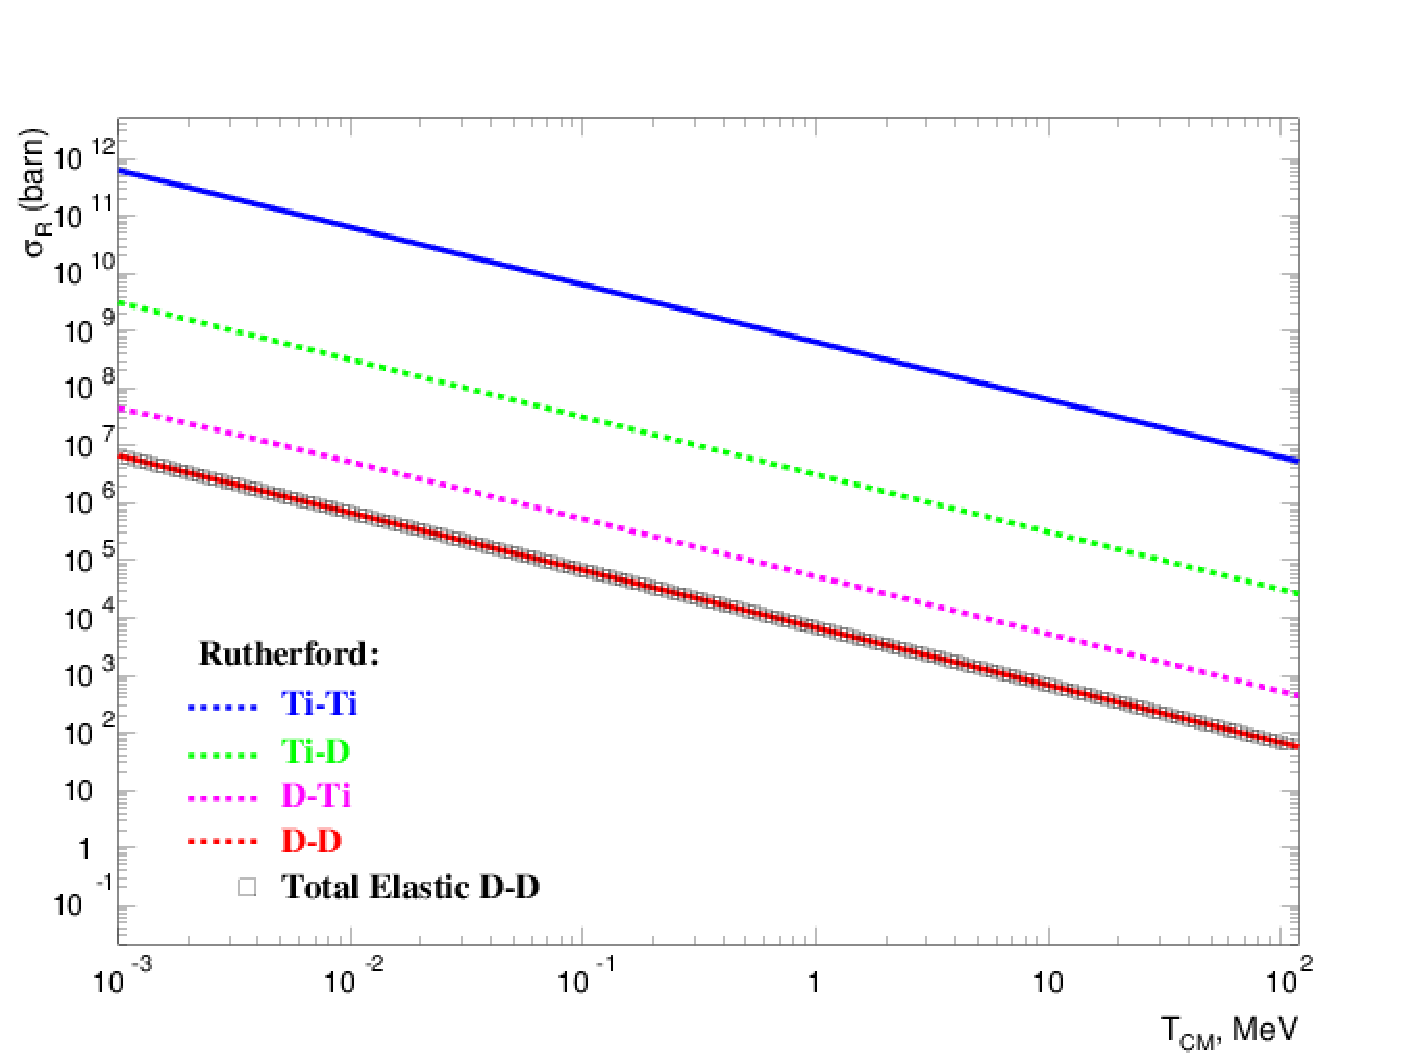
\includegraphics[width=0.99\linewidth]{images/integral_rutherford_d_ti_cross_sections.pdf}
  }
  \caption{Зависимости интегральных сечений D-D, D-Ti, Ti-D и Ti-Ti Резерфордовского рассеяния от кинетической энергии в системе центра масс $T_{CM}$.
  	Пустыми квадратами показано интегральное сечение аппроксимации экспериментальных данных дифференциального упругого D-D сечения из базы ядерных данных EXFOR, осуществленной в \cite{70/778-T}.}
  \label{fig:IntegralRutherfordDTiCrossSections}
\end{figure}

	Следует отметить, что при использовании аппроксимации дифференциального сечения упругого D-D рассеяния, полученной в \cite{70/778-T}, интегральное сечение в итоге не отличается от интегрального сечения Резерфордовского рассеяния.
	Это связано с тем, что, как видно из Рис. ~    \ref{fig:DifferenceOfElasticDDFromRutherfordDifferentialCrossSection}, отличие полученной аппроксимации дифференциального сечения упругого D-D рассеяния наблюдается только при угле рассеяния, близком к $\frac{\pi}{2}$.
	Поэтому нетрудно заметить, что вклад этого отличия в итоговое интегральное сечение пренебрежимо мал, т. к. дифференциальное сечение упругого рассеяния сильно падает от 0 до $\frac{\pi}{2}$.
	
	Т. к. рассматриваемый процесс упругий, $p_{CM}$ не меняется до и после взаимодействия, самая большая сложность в реализации конечного состояния этого процесса (на вход подана 1 частица, на выходе получаются  2) будет в генерации случайного значения $\cos{\theta_{CM}}$.
	Ниже будет описано как проводился розыгрыш по случайному числу от 0 до 1 случайного значения $\cos{\theta_{CM}}$.
	
	Т. к. рассматривается задача моделирования ион-ионного каскада в дейтериде титана, то налетающая частица может рассеяться на ядрах только 2 типов: дибо ядрах дейтерия, либо изотопов титана.
	Т. к. при моделировании ионного каскада мишень из дейтерида титана облучается потоком дейтронов, то возможные варианты рассеяния: D-D, D-Ti, Ti-D, Ti-Ti.
	Таким образом, получается всего 2 варианта рассеяния: рассеяние различных частиц (D-Ti, Ti-D) и рассеяние тождественных частиц (D-D и Ti-Ti).
	
	Перед тем как приступать к осуществлению процесса рассеяния налетающей частицы, необходимо проверить условие $|t|_{min} \leq |t|_{max}$.
	Если оно выполнено, можно переходить к рассеянию частицы.
	Если же нет, т. е. $|t|_{max} \leq |t|_{min}$, то интегралы $\int \limits^{|t|_{max}}_{|t|_{min}} \frac{d\sigma_R}{d|t|} \cdot d|t|$ будут отрицательными, что не имеет смысла, поэтому следует вернуть значение $\cos{\theta_{CM}}=1$, т. е. $\theta_{CM}=0$.
	Ситуация $|t|_{max}=4\cdot p^2_{CM} \leq |t|_{min}=2\cdot M \cdot E_{de}$ может возникнуть тогда, когда $p_{CM} \leq \sqrt{ \frac{1}{2} \cdot M \cdot E_{de} }$.
	Например, для D-D рассеяния эта ситуация возникает при $p_{CM} \leq 97$ кэВ, а для D-Ti -- при $p_{CM} \leq 1.5$ МэВ.
	
	При рассеянии различных частиц не возникает никаких затруднений: значение $|t|$ после рассеяния находится из соотношения $\int \limits^{|t|}_{|t|_{min}}=R \cdot \int \limits^{|t|_{max}}_{|t|_{min}} \frac{d\sigma_R}{d|t|} \cdot d|t|$, где $R$ -- псевдослучайное число от 0 до 1.
	При использовании (\ref{IntegralRutherfordCSDifferentParticles}) отсюда сразу получаются выражения
	
\begin{equation}
\label{TDifferentParticles}
\begin{aligned} 
   |t| = \frac{|t|_{min}}{1-R\cdot \left( 1-\frac{|t|_{min}}{|t|_{max}} \right)} 
\end{aligned}
\end{equation}

	и, т. к. $|t|=2\cdot p^2_{CM} \cdot \left( 1-\cos{\theta_{CM}} \right)$,
	
\begin{equation}
\label{CosThetCMDifferentParticles}
\begin{aligned} 
  \cos{ \theta_{CM}} = 1- \frac{|t|_{min}}{|t|_m \cdot \left( 1-R\cdot \left( 1-\frac{|t|_{min}}{|t|_{max}} \right) \right)},
\end{aligned}
\end{equation}

	где $|t|_{m}=2\cdot p^2_{CM}$ и $|t|_{max}=4\cdot p^2_{CM}$.
	
	Если рассеиваются одинаковые частицы, допустим Ti-Ti, D-D рассеяние здесь не рассматривается, оно будет рассмотрено ниже, то, как видно из выражения (\ref{DifferentialRutherfordCSEqualParticles}), в дифференциальном сечении присутствуют 3 слагаемых, интеграл от каждого из которых от $|t|_{min}$ до $|t|_m=2\cdot p^2_{CM}$ (т. к. рассеиваются тождественные частицы, то максимальный угол рассеяния $\theta_{CM}=\frac{\pi}{2}$ и максимальное значение переменной $|t|$ равно $|t|_m=2\cdot p^2_{CM}$, а не $|t|_{max}=4\cdot p^2_{CM}$) должен рассматриваться отдельно.
	Т. е. как бы есть 3 ``канала'' рассеяния, с помощью случайного числа от 0 до 1 по соотношению интегралов происходит выбор в каком канале рассеиваться, и по ещё одному случайному числу от 0 до 1 происходит рассеяние -- получается значение $|t|$ и $\cos{\theta_{CM}}$.
	
	Здесь возникает определённая сложность: интеграл от интерференционного члена в (\ref{IntegralRutherfordCSEqualDD}) может оказаться отрицательным, что вносит ошибку в определение того, какой канал выиграет.
	
	Чтобы этого не происходило, было принято решение определить величину $|t|_{mid}=\frac{|t|_{max}}{1+e^{\frac{\pi}{2} \cdot \frac{\beta^r_{CM}}{\alpha}}}$.
	Величина $|t|_{mid}$ определялась из условия того, чтобы фаза синуса в интеграле от интерференционного слагаемого в (\ref{IntegralRutherfordCSEqualParticles}) была меньше $\frac{\pi}{2}$, т. е. чтобы интеграл от интерференционного слагаемого не становился отрицательным.
	Таким образом, получалось, что при $|t| > |t|_{mid}$ интеграл от интерференционного члена в дифференциальном сечении был неотрицательным.
	
	Определение того, какой ``канал'' Резерфордовского рассеяния тождественных частиц выиграет, происходило следующим образом.
	Вычислялись интегралы от 1-го и 2-го членов: $I_1=I_2=\frac{\pi}{p^2_{CM}} \cdot \left( m \alpha \hbar c Z^2 \right)^2 \cdot \left( \frac{1}{|t|_{min}} - \frac{1}{|t|_{max}-|t|_{min}} \right)$, т. к. частицы тождественные, то $m=M$ и $z=Z$.
	Интеграл от интерференционного члена в дифференицальном сечении (\ref{DifferentialRutherfordCSEqualParticles}) определялся как интеграл от $|t|_{mid}$ до $|t|_{max}$.
	Если $|t|_{mid} > |t|_{max}$, он был равен нулю.
	Если же $|t|_{mid} < |t|_{min}$, то он считался от $|t|_{min}$ до $|t|_{max}$.
	С помощью равномерно распределённого случайного числа от 0 до 1 определялось, по какому каналу будет происходить генерация случайных $|t|$ и $\cos{\theta_{CM}}$.
	
	Если выигрывал 1-ый канал, то $|t|$ определялось как
	
\begin{equation}
\label{Channel1TEqualParticles}
\begin{aligned} 
  |t| = \frac{1}{ \frac{1-R}{|t|_{min}} + \frac{R}{|t|_m} },
\end{aligned}
\end{equation}

	если 2-ой, то как
	
\begin{equation}
\label{Channel2TEqualParticles}
\begin{aligned} 
  |t| = |t|_{max} - \frac{1}{ \frac{1-R}{|t|_{max}-|t|_{min}} + \frac{R}{|t|_m} },
\end{aligned}
\end{equation}

	а если 3-ий, то как
	
\begin{equation}
\label{Channel3TEqualParticles}
\begin{aligned} 
  |t| = \frac{ |t|_{max} \cdot e^A}{1+e^A},
\end{aligned}
\end{equation}

	где
	
\begin{equation}
\label{Channel3TEqualParticlesA}
\begin{aligned} 
  A = \frac{ \beta^r_{CM} }{\alpha} \cdot \arcsin{ \Biggl( \biggl( \sin{ \frac{\alpha}{\beta^r_{CM}} \cdot \ln{ \Bigl( \frac{|t|_{min}}{|t|_{max}-|t|_{min}} \Bigr) } \biggr) } \cdot \left( 1-R \right) \Biggr) }.
\end{aligned}
\end{equation}

	Здесь $R$ -- равномерно распределённое случайное число от 0 до 1, а $|t|$ разыгрывается от $|t|_{min}$ не до $|t|_{max}=4\cdot p^2_{CM}$, а до $|t|_m=2\cdot p^2_{CM}$, т. е. не до $\theta_{CM}=\pi$, а до $\theta_{CM}=\frac{\pi}{2}$, потому что рассеиваются тождественные частицы.
	
	Далее, из полученного сгенерированного случайного значения $|t|$ получалось значение $\cos{ \theta_{CM} }=1-\frac{|t|}{2\cdot p^2_{CM}}$.
	
	При моделировании упругого D-D расеяния ситуация была несколько сложнее.
	Как упоминалось в разделе \ref{ValElasticDD}, в отчёте \cite{70/778-T} была получена аппроксимация упругого дифференциального сечения D-D рассеяния, отличающаяся от Резерфордовского дифференциального сечения только при максимальных углах рассеяния в системе центра масс, близких к $\frac{\pi}{2}$.
	Она изображена на Рис. ~\ref{fig:DifferenceOfElasticDDFromRutherfordDifferentialCrossSection} в дважды логарифмическом масштабе, где по оси абсцисс отложена безразмерная переменная $1-\cos{ \theta_{CM}}$.
	
	
\begin{figure}[ht]
  {
     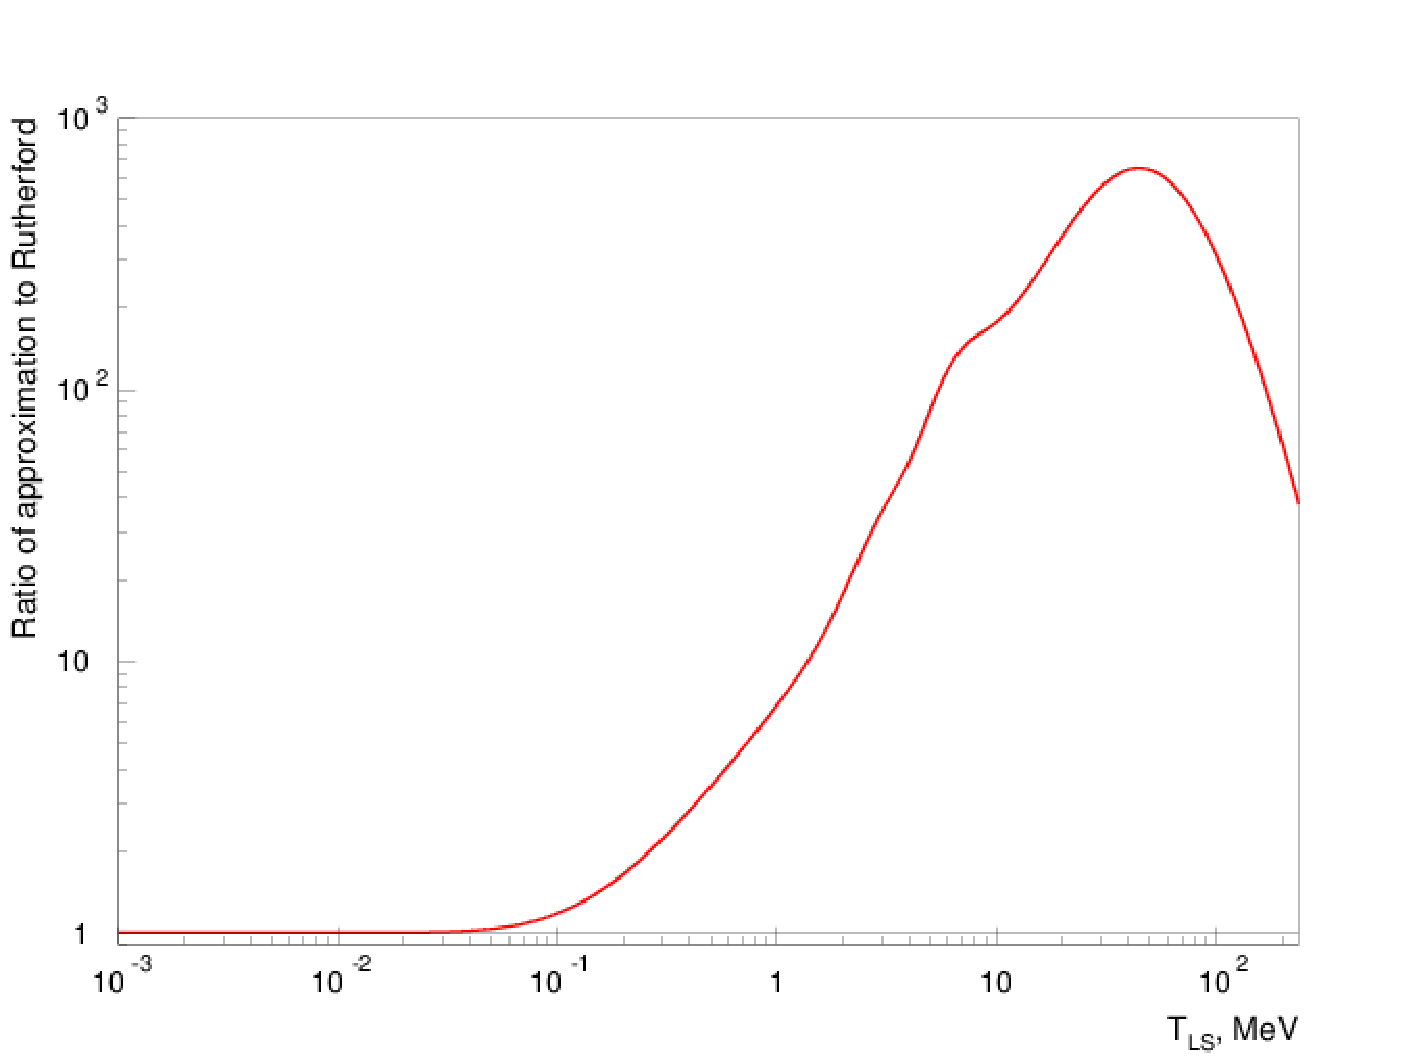
\includegraphics[width=0.5\linewidth]{images/ratio_of_elastic_dd_at_90_grades.pdf}
     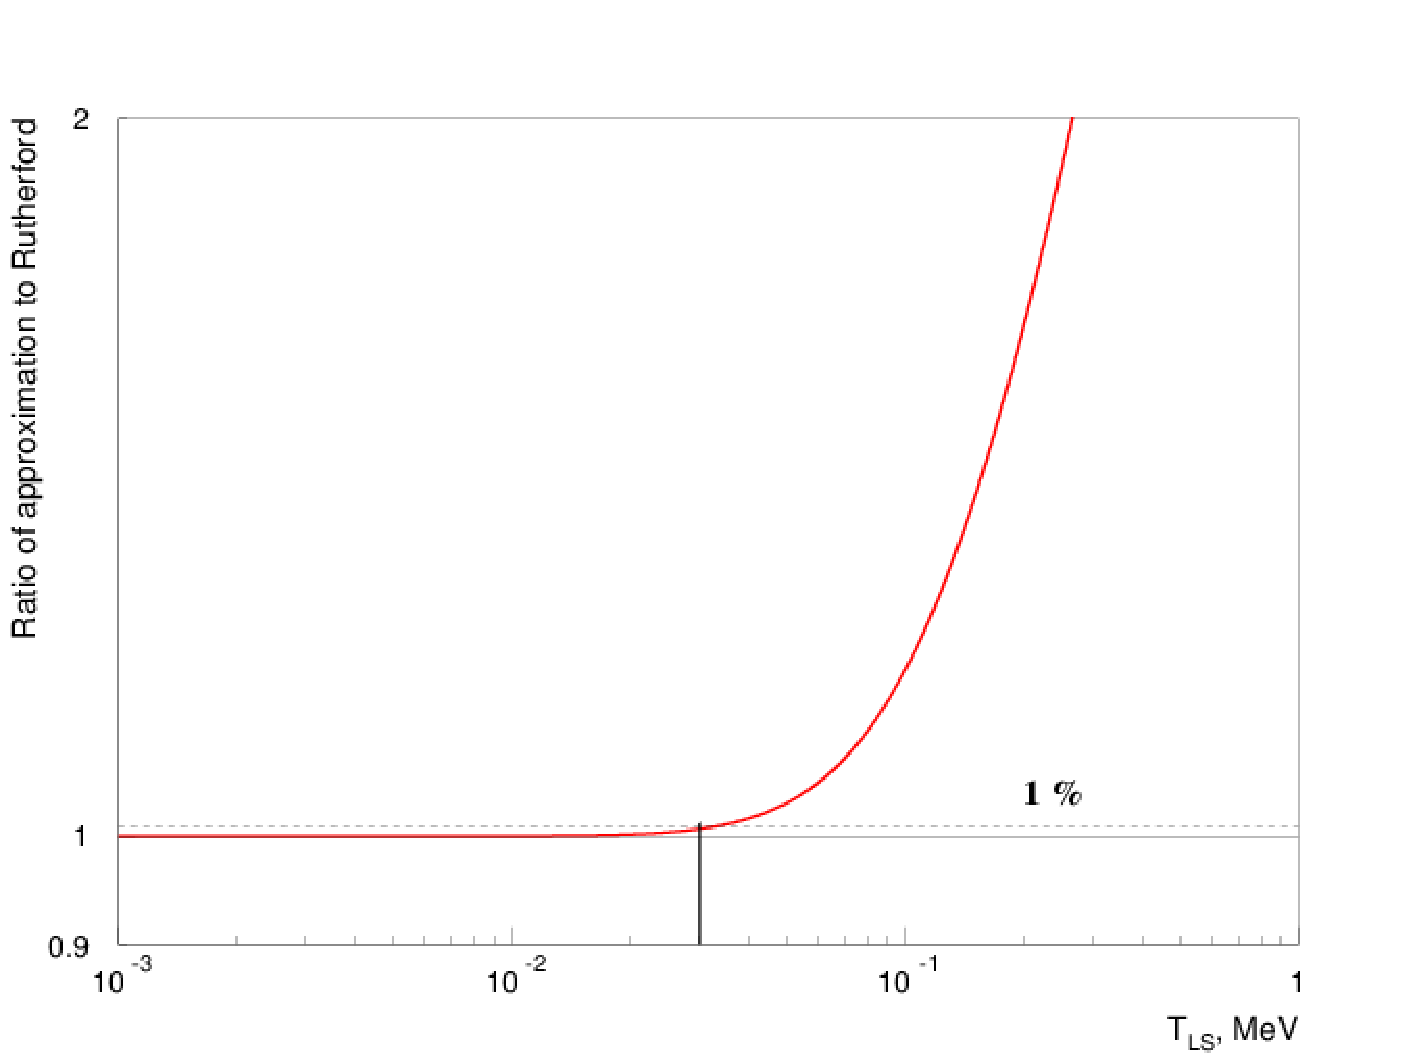
\includegraphics[width=0.5\linewidth]{images/ratio_of_elastic_dd_at_90_grades_find_1_percent_diff.pdf}
  }
  \caption{\textit{\textbf{Слева:}} Отношение полученной в \cite{70/778-T} и изображённой на Рис. ~\ref{fig:DifferenceOfElasticDDFromRutherfordDifferentialCrossSection} аппроксимации дифференциального сечения упругого D-D рассеяния при угле рассеяния $\theta_{CM}=\frac{\pi}{2}$ к значению дифференциального сечения Резерфордовского рассеяния при $\theta_{CM}=\frac{\pi}{2}$ при одной и той же кинетической энергии налетающего дейтрона $T_{LS}$.
  \textit{\textbf{Справа:}} То же отношение, увеличенное в области, где оно только начинает отличаться от 1 так, чтобы можно было видеть начиная с какой $T_{LS}$ отличие составляет не менее 1 \%.}
  \label{fig:RatioOfElasticDDAt90Grades}
\end{figure}	
	
	
	Как хорошо видно из Рис. ~\ref{fig:RatioOfElasticDDAt90Grades}, при $T_{LS} \leq 10$ кэВ полученная аппроксимация никак не отличается от дифференциального Резерфордовского сечения.
	
	В то же время, необходимо было выяснить, где при $T_{LS}>10$ кэВ аппроксимация совпадает с дифференциальным Резерфордовским сечением, а где от него отличается. 
	При взгляде на Рис. ~\ref{fig:DifferenceOfElasticDDFromRutherfordDifferentialCrossSection} затруднительно сразу ответить на этот вопрос. 
	Было проведено исследование, в ходе которого для каждого из значений $T_{LS}$ на Рис. ~\ref{fig:DifferenceOfElasticDDFromRutherfordDifferentialCrossSection} было найдено, начиная с какого значения $1-\cos{ \theta_{CM} }$ между аппроксимацией и дифференциальным Резерфордовским сечением имеется не менее чем 10 \% отличие. 
	Было выяснено, что полученные для каждого из значений $T_{LS}$ на Рис. ~\ref{fig:DifferenceOfElasticDDFromRutherfordDifferentialCrossSection} величины $1-\cos{ \theta_{CM} }$, начиная с которых отличие аппроксимации от Резерфордовского дифференциального сечения составляет не менее 10 \%, группируются вокруг значения $10^{-3}$. 
	Так что с неплохой точностью можно считать, что при любых $T_{LS}$ в рассматриваемом диапазоне $10$ кэВ $\leq T_{LS} \leq 250$ МэВ (самая большая кинетическая энергия налетающего дейтрона $T_{LS}$ в экспериментальных данных, использовавшихся  для аппроксимации, равняется 231.8 МэВ, поэтому мы приближённо считаем, что верхняя граница применимости полученной аппроксимации по $T_{LS}$ равна 250 МэВ) упругого D-D рассеяния при $1-\cos{ \theta_{CM}} < 10^{-3}$ нет никакого отличия между полученной аппроксимацией и Резерфордовским дифференциальным сечением D-D рассеяния, а при $1-\cos{ \theta_{CM}} \geq 10^{-3}$ чем ближе к $\theta_{CM}=\frac{\pi}{2}$, тем больше отличие аппроксимации от дифференциального сечения рассеяния Резерфорда и поэтому, для того чтобы точнее описывать угловое распределение D-D упругого рассеяния, нужно использовать полученную аппроксимацию.
	
	Поэтому упругое D-D рассеяние описывалось следующим образом.
	Если кинетическая энергия налетающего дейтрона $T_{LS}$ была меньше 10 кэВ, считалось, что в этой области есть только Резерфордовское дифференциальное сечение рассеяния тождественных частиц, и случайный $\cos{\theta_{CM}}$ генерировался как только что было описано выше.
	Если же $T_{LS}$ была больше 10 кэВ, то в рамках процесса упругого ион-ионного рассеяния интегральное сечение упругого D-D рассеяния вычислялось как интеграл от Резерфордовского дифференциального сечения рассеяния тождественных частиц от $|t|_{min}$ до $10^{-3}\cdot |t|_{m}=2\cdot 10^{-3}\cdot p^2_{CM}$.
	Аналогично, и случайное значение $|t|$ разыгрывалось от $|t|_{min}$ до $10^{-3}\cdot |t|_m$.
	
	Область $10^{-3} \cdot |t|_m \leq |t|_m$ для упругого D-D рассеяния разыгрывалась в отдельном процессе упругого D-D рассеяния, который будет описан в следующем разделе.
	
	Применительно к задаче моделирования ионного каскада в мишени из дейтерида титана, вызванного облучением мишени потоком дейтронов, на вход рассматриваемому процессу подавался вектор 4-импульса налетающего иона, а на выходе получались 4-импульсы рассеянного иона и ядра отдачи.


\subsection{Реализация дискретного процесса упругого D-D рассеяния.}
\label{ElasticDDScatteringRealization}

	Процесс упругого D-D рассеяния в области $T_{LS} \geq 10$ кэВ реализовывался при использовании аппроксимации дифференциального сечения упругого D-D рассеяния, полученной в \cite{70/778-T}.
	
	В области $10^{-3} \leq 1-\cos{\theta_{CM}} \leq 1$ слева направо задавалась логарифмическая шкала оси абсцисс и справа налево проводилось интегрирование $\int \limits^{|t|_m}_{10^{-3}\cdot |t|_m} \frac{d\sigma^{approx}}{d|t|} \cdot d|t|$.
	Т. к. $\frac{d\sigma^{approx}}{d|t|} \sim \frac{1}{|t|^2}$, поэтому интегрирование проводилось справа налево, чтобы учесть малый вклад правых логарифмических бинов.
	Ведь если проводить интегрирование слева направо, в самых правых логарифмических бинах, где величина значений функции на порядки меньше её значений в самых левых бинах, значения нормированных частичных сумм будут очень мало отличаться от 1 и друг от друга.
	Интегрирование справа налево позволяет избавиться от этой проблемы.
	
	Интегральные сечения данного процесса определялись как $2 \cdot \int \limits^{|t|_m}_{10^{-3}\cdot |t|_m} \frac{d\sigma^{approx}}{d|t|} \cdot d|t|$, т. к. рассеиваются тождественные частицы, а значит, дифференциальное сечение рассеяния симметрично относительно угла рассеяния $\theta_{CM}=\frac{\pi}{2}$.
	Так же в ходе интегрирования были получены частичные суммы, соответствующие интегралам $\int \limits^{|t|_m}_{|t|_i} \frac{d\sigma^{approx}}{d|t|} \cdot d|t|$, где $|t|_i$ -- левые границы логарифмических бинов, а $i=0..N_{bin}-1$, $N_{bin}$ -- число бинов, равное 128, частичные суммы делились на полный интеграл от $|t|_{min}$ до $10^{-3} \cdot |t|_m$, в результате чего для каждого из 100 значений $T_{LS}$ в диапазоне 10 кэВ $\leq$ 250 МэВ получался набор данных ($1-cos{\theta_{CM}}$, частичные суммы).
	
	Розыгрыш случайного значения $\cos{\theta_{CM}}$ проводился следующим образом.
	Сначала по значению $T_{LS}$ налетающего дейтрона при использовании бинарного поиска определялись 2 соседних набора частичных сумм, соответствующие значениям $T_{LS}$, между которыми находится $T_{LS}$ налетающего дейтрона.
	Далее, с помощью равномерно распределённого случайного числа от 0 до 1 и квадратичной интерполяции определялось значение $\cos{\theta_{CM}}$.
	
	На вход данному процессу подавался вектор 4-импульса налетающего дейтрона, а на выходе получались 2 4-импульса -- рассеянного дейтрона и дейтрона отдачи.
	Если налетающая частица не была дейтроном, интегральное сечение процесса было равно 0, и процесс упругого D-D рассеяния не осуществлялся.
	
	
\subsection{Непрерывные процессы многократного рассеяния и $\frac{dE}{dx}$.}
\label{MSanddEdxRealization}

	Также в ходе моделирования присутствовали непрерывные (которые происходят не дискретно в вершине взаимодействия, а непрерывно вдоль трека частицы) процессы многократного рассеяния и линейных электронных потерь энергии $\frac{dE}{dx}$ частицы в материале мишени.
	
	Непрерывный процесс многократного рассеяния подробно описан в разделе \ref{ValMS}.
	Он приводит к изменению на каждом шаге моделирования направления вектора импульса каждой заряженной частицы, проходящей через материал мишени на некий малый угол, величина которого определялась аппроксимацией функции плотности вероятности углового распределения многократного рассеяния (\ref{MSApproximationFunction}) при должном скейлинге, описанном в разделе \ref{subValMS2}.
	
	Непрерывный процесс линейных электронных потерь энергии заряженной частицы на каждом шаге моделирования подробно описан в разделе \ref{ValdEdx}.
	Он просто приводит к уменьшению энергии каждой заряженной частицы на шаге в соответствии с $E=E-\frac{dE}{dx} \cdot \rho_{TiD_2} \cdot l$, где $l$ -- длина пробега частицы на шаге.

	
\clearpage{}
\section{Моделирование выхода нейтронов при облучении мишени из дейтерида титана интенсивным потоком дейтронов.}
\label{NeutronOutput}

	Перед моделированием ионного каскада в мишени из дейтерида титана необходимо было удостовериться, что в результате облучения мишени из дейтерида титана интенсивным потоком дейтронов с начальной кинетической энергией 100 кэВ правильным образом -- с согласующейся с результатами экспериментов вероятностью -- генерируются нейтроны в результате реакции неупругого D-D рассеяния.
	
	Т. к. для моделирования выхода нейтронов интересны только дейтроны, то все вторичные частицы, получающиеся в ходе процессов непругой D-D реакции и упругого ион-ионного рассеяния: протоны, тритоны, ядра $^3_2$He и изотопов титана считались и исключались из моделирования.
	Нейтроны тоже подсчитывались и исключались из моделирования.  

\subsection{Пробег дейтронов в дейтериде титана в зависимости от энергии остановки дейтерия.}
\label{DeuteronRangesInTiD2}
	
	Для ускорения моделирования, а, главным образом, потому что сечение неупругой D-D реакции дейтронов быстро падает с уменьшением их энергии, и ожидать выхода нейтронов с $T_{LS} \leq 10-20$ кэВ бессмысленно, при $T_{LS} \leq 10$ кэВ дейтроны исключались из моделирования.
	
	Для того чтобы знать толщину мишени, на которой все дейтроны, запущенные с энергией 100 кэВ, гарантированно остановятся, необходимо было подсчитать длину пробега дейтронов материале мишени, равную $\int \limits^{T^{max}_{LS}}_{T^{min}_{LS}} \frac{dx}{dE} \cdot dE$, где использовалась полученная аппроксимация $\frac{dE}{dx}$ для протонов в дейтериде титана и скейлинг, описанные в разделе \ref{ValdEdx}, и $T^{max}_{LS}=100$ кэВ, а $T^{min}_{LS}=10$ кэВ. В результате численного интегрирования было получено значение 0.865 мкм.
	
	Было интересно посмотреть, как зависит длина пробега от ``энергии обрезания'' $T_{CUT}$, которая была положена равной 10 кэВ.
	Если изменять величину $T_{CUT}$, то получающаяся зависимость длины пробега дейтронов в мишени из дейтерида титана от $T_{CUT}$ показана на Рис. ~\ref{fig:RangesOfDeuteronsInTiD2}.
	  
\begin{figure}[ht]
  {
     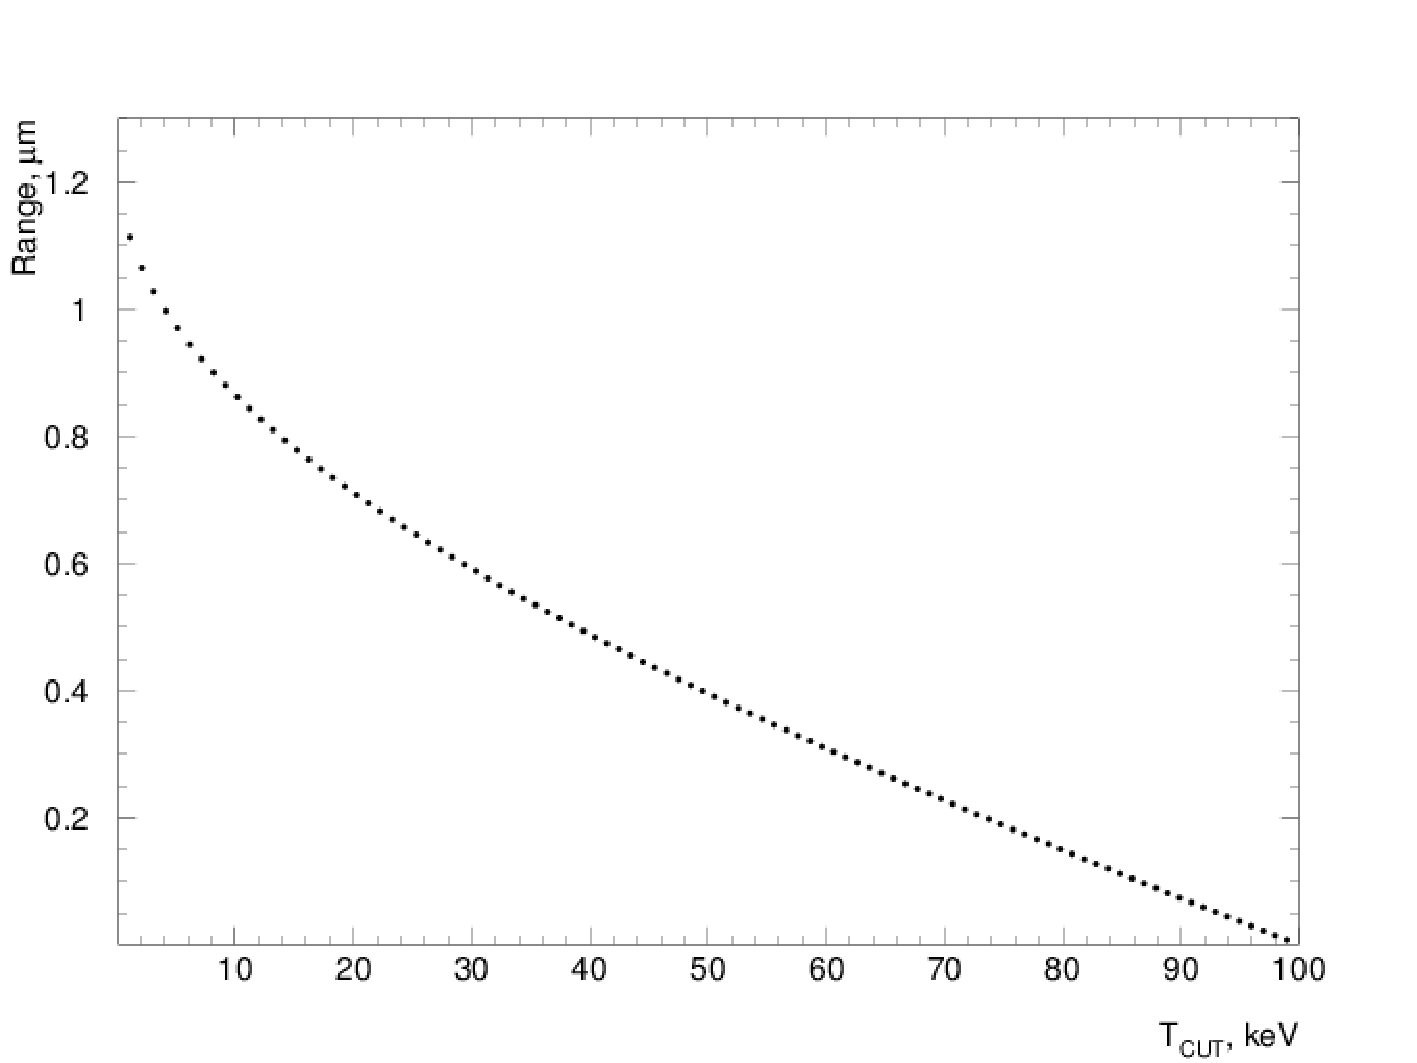
\includegraphics[width=0.99\linewidth]{images/ranges.pdf}
  }
  \caption{Зависимость длины пробега дейтронов с начальной кинетической энергией 100 кэВ в мишени из дейтерида титана от значения кинетической энергии обрезания $T_{CUT}$.}
  \label{fig:RangesOfDeuteronsInTiD2}
\end{figure}

\subsection{Средние длины пробегов дейтронов в дейтериде титана в зависимости от кинетической энергии.}
\label{DeuteronMeanRangesDependenceOnEnergyInTiD2}

	С целью узнать зависимость средних длин свободного пробега дейтронов в процессах упругого ион-ионного рассеяния и реакции неупругого D-D рассеяния было произведено моделирование, в результате которого были получены гистограммы распределения средних длин пробега дейтронов в данных процессах в зависимости от их кинетической энергии.
	Они изображены на Рис. ~\ref{fig:RangesOfDeuteronsInInelasticAndElasticProcesses}.
	При составлении данных гистограмм оставлялся включенным только интересующий процесс, сечения остальных процессов фиктивно ставились равными 0.  
	
\begin{figure}[ht]
  {
     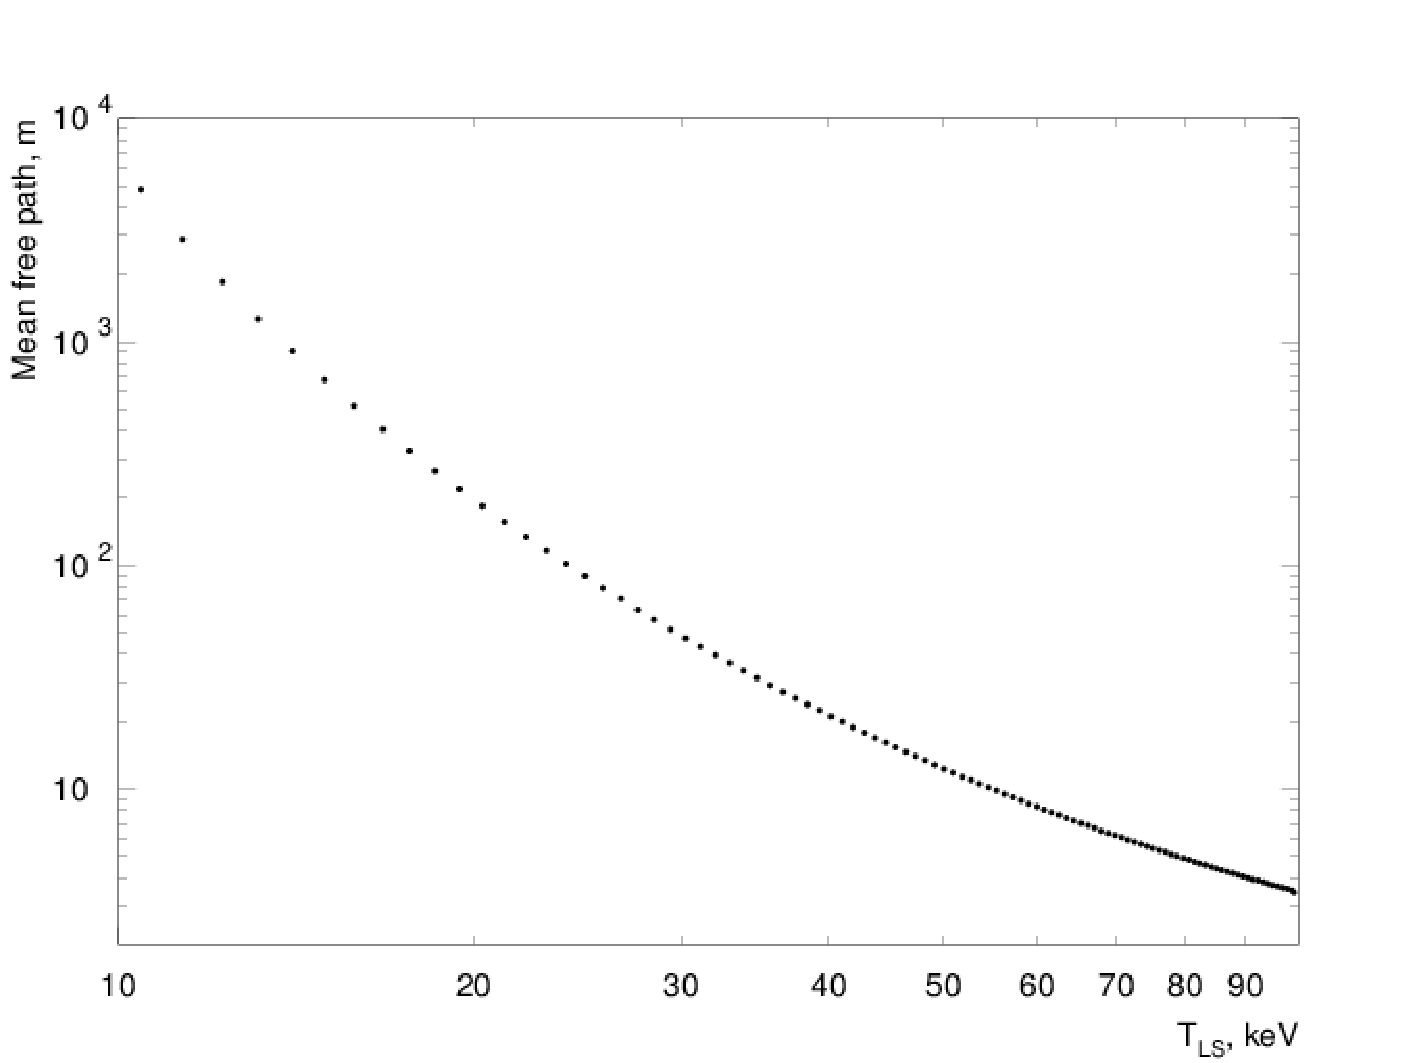
\includegraphics[width=0.5\linewidth]{images/fluence_inelastic.pdf}
     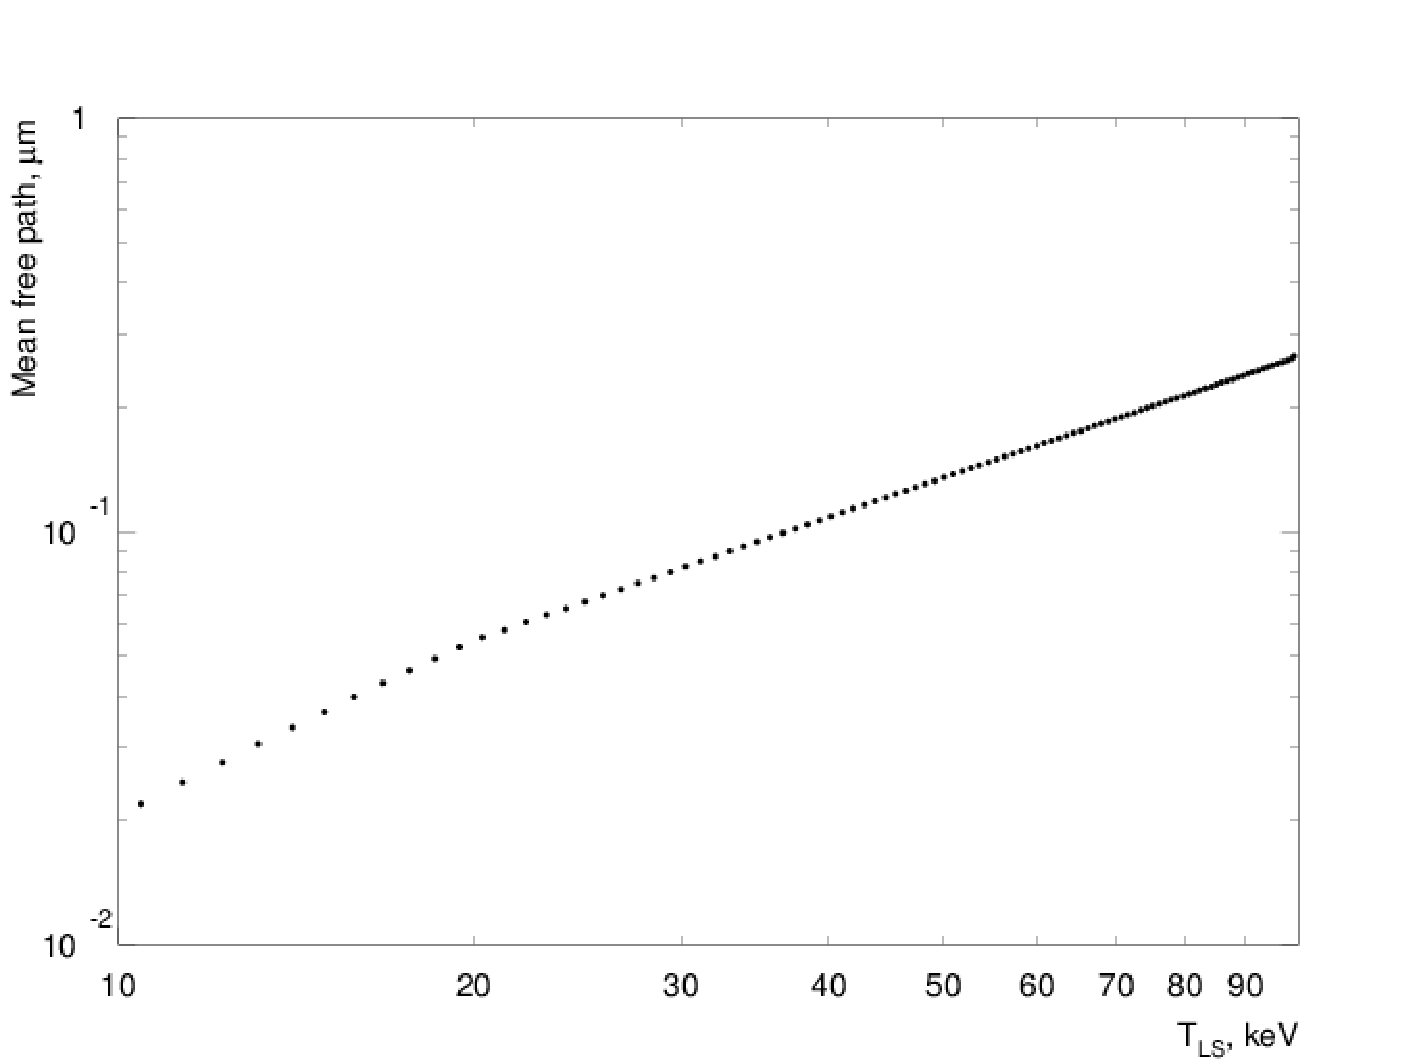
\includegraphics[width=0.5\linewidth]{images/fluence_elastic.pdf}
  }
  \caption{Зависимость средней длины свободного пробега дейтронов в дейтериде титана в зависимости от их кинетической энергии в процессах: \textbf{\textit{слева}} -- реакции неупругого D-D рассеяния, \textbf{\textit{справа}} -- упругого ион-ионного рассеяния.}
  \label{fig:RangesOfDeuteronsInInelasticAndElasticProcesses}
\end{figure}
	
\subsection{Вероятность нейтронного выхода на 1 запущенный дейтрон.}
\label{ProbabilityOfNeutronOutputPer1Deuteron}

	Зная распределение средних длин свободного пробега в полноценном процессе моделирования, когда включены все процессы -- и неупругая D-D реакция, и упругое ион-ионное рассеяние -- можно узнать вероятность нейтронного выхода на 1 запущенный дейтрон.
	
	Для этого нужно из получившегося в результате моделирования, в котором включены все процессы, распределения средних длин свободного пробега дейтронов в зависимости от их кинетической энергии посчитать величину $\frac{dl}{dE}$  и свернуть её с $n_{TiD_2} \cdot \sigma_{Inelastic\,DD}$. Это было сделано, в результате чего была получена вероятность нейтронного выхода на 1 запущенный дейтрон:
	
\begin{equation}
\label{ProbabilityOfNeutronOutputPer1Deuteron}
\begin{aligned} 
  P = \int \limits^{T^{max}_{LS}}_{T^{min}_{LS}} \frac{dl}{dE} \cdot n_{TiD_2} \cdot \sigma_{Inelastic\,DD} \cdot dE = 2.7 \cdot 10^{-8}.
\end{aligned}
\end{equation}

\subsection{Нейтронный выход в ходе моделирования.}
\label{NeutronOutputInModelling}

	В результате моделирования нейтронного выхода от $N_D$ запущенных дейтронов разрабатываемым программным кодом был получен следующий результат:
	
\begin{tabular}{|c|c|c|}
 \hline 
 $N_D$ & Общее число непругих D-D реакций & Выход нейтронов \\ 
 \hline 
 $10^6$ & 0 & 0 \\ 
 \hline 
 $10^7$ & 2 & 2 \\ 
 \hline 
 $10^8$ & 12 & 4 \\ 
 \hline 
 $10^9$ & 153 & 72 \\ 
 \hline 
 \end{tabular}
 
 
 


	TODO:
	
	1) На Рис. 1 и 2 исправить подписи осей: W(x) и D(x).
	
	2) Рисунки распределения многократного рассеяния для ионов дейтерия и титана получены для 		неправильного скейлинга $z \cdot \frac{E^2_{LS}}{p^4_{LS}}$. По-хорошему, надо бы перестроить картинки для правильного скейлинга $z^2 \cdot \frac{E^2_{LS}}{p^4_{LS}}$.
	
	3) Перестроить подпись на картинке 5. По оси абсцисс $\theta$, а не Bin number.
 

	
\clearpage
\section{Заключение}
\label{Conclusion}
% magic phrase for the quarterly report
  В результате работ, выполненных в ФГУП ВНИИА в первом квартале 2019 года в рамках темы "СОЧЕТАНИЕ"\ : "Совершенствование физических моделей взаимодействия излучений с веществом"\ появилась возможность моделирования ионных каскадов, индуцированных прохождением нейтронов деления через конструкционные материалы ядерных установок.
  В новой программе ТРТ3 моделирование многократного рассеяния и дискретного упругого ион-ионного рассеяния проводится на новом качественном уровне, исключая двойной счёт, связанный с использованием усреднённых ядерных потерь энергии в веществе.
  Новые возможности открывают перспективу более точного и детального моделирования процессов, определяющих радиационную стойкость материалов, однако реального результата в этом направлении можно добиться только после сопряжения программного комплекса ТРТ с программами молекулярной динамики.
  
\clearpage
\bibliography{reptptgeom}
% now with bibtex


\end{large}
\end{document}
